\documentclass [norsk,a4paper,twoside]{article}\usepackage[]{graphicx}\usepackage[]{color}
%% maxwidth is the original width if it is less than linewidth
%% otherwise use linewidth (to make sure the graphics do not exceed the margin)
\makeatletter
\def\maxwidth{ %
  \ifdim\Gin@nat@width>\linewidth
    \linewidth
  \else
    \Gin@nat@width
  \fi
}
\makeatother

\definecolor{fgcolor}{rgb}{0.345, 0.345, 0.345}
\newcommand{\hlnum}[1]{\textcolor[rgb]{0.686,0.059,0.569}{#1}}%
\newcommand{\hlstr}[1]{\textcolor[rgb]{0.192,0.494,0.8}{#1}}%
\newcommand{\hlcom}[1]{\textcolor[rgb]{0.678,0.584,0.686}{\textit{#1}}}%
\newcommand{\hlopt}[1]{\textcolor[rgb]{0,0,0}{#1}}%
\newcommand{\hlstd}[1]{\textcolor[rgb]{0.345,0.345,0.345}{#1}}%
\newcommand{\hlkwa}[1]{\textcolor[rgb]{0.161,0.373,0.58}{\textbf{#1}}}%
\newcommand{\hlkwb}[1]{\textcolor[rgb]{0.69,0.353,0.396}{#1}}%
\newcommand{\hlkwc}[1]{\textcolor[rgb]{0.333,0.667,0.333}{#1}}%
\newcommand{\hlkwd}[1]{\textcolor[rgb]{0.737,0.353,0.396}{\textbf{#1}}}%
\let\hlipl\hlkwb

\usepackage{framed}
\makeatletter
\newenvironment{kframe}{%
 \def\at@end@of@kframe{}%
 \ifinner\ifhmode%
  \def\at@end@of@kframe{\end{minipage}}%
  \begin{minipage}{\columnwidth}%
 \fi\fi%
 \def\FrameCommand##1{\hskip\@totalleftmargin \hskip-\fboxsep
 \colorbox{shadecolor}{##1}\hskip-\fboxsep
     % There is no \\@totalrightmargin, so:
     \hskip-\linewidth \hskip-\@totalleftmargin \hskip\columnwidth}%
 \MakeFramed {\advance\hsize-\width
   \@totalleftmargin\z@ \linewidth\hsize
   \@setminipage}}%
 {\par\unskip\endMakeFramed%
 \at@end@of@kframe}
\makeatother

\definecolor{shadecolor}{rgb}{.97, .97, .97}
\definecolor{messagecolor}{rgb}{0, 0, 0}
\definecolor{warningcolor}{rgb}{1, 0, 1}
\definecolor{errorcolor}{rgb}{1, 0, 0}
\newenvironment{knitrout}{}{} % an empty environment to be redefined in TeX

\usepackage{alltt}
\addtolength{\hoffset}{-0.5cm}
\addtolength{\textwidth}{1cm}
\addtolength{\voffset}{-1cm}
\addtolength{\textheight}{2cm}


%for nice looking tabs
\usepackage{booktabs}

\usepackage[norsk]{babel}
\usepackage[utf8x]{inputenc}
\usepackage{textcomp}
\usepackage{fancyhdr}
\pagestyle{fancy}
\usepackage{amsmath}
\usepackage{rotating} %add rotating for plain tables
\usepackage{pdflscape} %add rotating/landcape for pdf

%bytte font
\renewcommand{\familydefault}{\sfdefault}

%setter grå skrift fremfort sort
\usepackage{xcolor}
\usepackage{graphicx}
\usepackage[pdftex, colorlinks, linkcolor=OffBlaa3, urlcolor=OffBlaa3]{hyperref}
\newcommand{\kommentar}[1]{\cbstart\textcolor{red}{#1\cbend}}
\IfFileExists{upquote.sty}{\usepackage{upquote}}{}
\begin{document}





\begin{knitrout}
\definecolor{shadecolor}{rgb}{0.969, 0.969, 0.969}\color{fgcolor}\begin{kframe}


{\ttfamily\noindent\itshape\color{messagecolor}{\#\# The following objects are masked \_by\_ .GlobalEnv:\\\#\# \\\#\#\ \ \ \  ASA, HovedInngrep, UforetrygdPre}}\end{kframe}
\end{knitrout}


\begin{knitrout}
\definecolor{shadecolor}{rgb}{0.969, 0.969, 0.969}\color{fgcolor}\begin{kframe}


{\ttfamily\noindent\bfseries\color{errorcolor}{\#\# Error in sprintf("{}\%.0f"{}, (N1aar - sum(NakkeData1aar\$ErMann))/Ntot1aarNakke * : object 'N1aar' not found}}\end{kframe}
\end{knitrout}


\section{Forbruksrater av rygg- og nakkekirurgi i Norge (kilde: NPR/SSB)}
Variasjon i forbruksrater av rygg og nakkekirurgi mellom regioner kan 
gjenspeile ulik tilgjengelighet til helsetjenesten, men også praksisvariasjon som kan
representere i kvalitetsforskjeller i behandlingstilbudet. Figur \ref{fig:AA_Nakkekirurgi_BoRHF1}, \ref{fig:AA_Ryggkirurgi_BoHF1} og \ref{fig:AA_Ryggkirurgi_BoRHF1} viser at det
er forskjeller i forbruksrater mellom ulike boområder i Norge. Disse kan ikke
forklares ut fra forskjeller i sykelighet. Forbruksraten er spesielt lav i boområdet til
Helse Nord, både når det gjelder nakke og ryggkirurgi, mens Helse Vest har gjennomgående høyest operasjonsrate. Forskjellene er størst for nakkekirurgi.

\begin{figure}[ht]
\scalebox{0.9}{\includegraphics{Figurer/AA_Ryggkirurgi_BoRHF1.pdf}}
\caption{Kjønns- og aldersstandardiserte rater pr. 100 000 innbyggere, ryggkirurgi, 20 - 85 år, RHf’enes opptaksområder, 2012-2017. Gjennomsnitt i perioden (søyler) og enkeltår (punkter).}
\label{fig:AA_Ryggkirurgi_BoRHF1}
\end{figure}

\begin{figure}[ht]
\scalebox{0.9}{\includegraphics{Figurer/AA_Ryggkirurgi_BoHF1.pdf}}
\caption{Kjønns- og aldersstandardiserte rater pr. 100 000 innbyggere, ryggkirurgi, 20 - 85 år, helseforetakenes opptaksområder, 2012-2017. Gjennomsnitt i perioden (søyler) og enkeltår (punkter).}
\label{fig:AA_Ryggkirurgi_BoHF1}
\end{figure}


\begin{figure}[ht]
\scalebox{0.9}{\includegraphics{Figurer/AA_Nakkekirurgi_BoRHF1.pdf}}
\caption{Kjønns- og aldersstandardiserte rater pr. 100 000 innbyggere, nakkekirurgi, 20 - 85 år, RHf’enes opptaksområder, 2012-2017. Gjennomsnitt i perioden (søyler) og enkeltår (punkter).}
\label{fig:AA_Nakkekirurgi_BoRHF1}
\end{figure}

\begin{figure}[ht]
\scalebox{0.9}{\includegraphics{Figurer/AA_Nakkekirurgi_BoHF1.pdf}}
\caption{Kjønns- og aldersstandardiserte rater pr. 100 000 innbyggere, nakkekirurgi, 20 - 85 år, Hf’enes opptaksområder, 2012-2017. Gjennomsnitt i perioden (søyler) og enkeltår (punkter).}
\label{fig:AA_Nakkekirurgi_BoHF1}
\end{figure}


\clearpage



\section{Oppsummeringstall for NKR}

\begin{kframe}


{\ttfamily\noindent\bfseries\color{errorcolor}{\#\# Error in gsub("{}\$"{}, "{}\textbackslash{}\textbackslash{}\$"{}, result, fixed = TRUE): input string 1 is invalid UTF-8}}\end{kframe}


\subsection{Degenerativ rygg}

Tabell \ref{tab:AntReg} viser antall 
registreringer gjort ved de respektive avdelinger hvert år. Vi ser at det er  
47 avdelinger som registrerer og at det i perioden 2011 til 2017 totalt er registrert 5810 
operasjoner. Av disse er 52.7\% utført på menn og 47.3\% på kvinner.
Siste nakkeinngrep registrert i datauttrekket som ligger til grunn for denne rapporten, ble utført 
2017-12-30. I peroden før 2010, det vil si fra og med 2007 til og med 2009 er det 
registrert 5832 operasjoner til NKR. 
\par

Flere enheter har hatt en stor og gledelig økning av antall registreringer til NKR, degenerativ rygg. Spesielt gjelder dette Kristiansund, Larvik , Førde og Ullevål (nevrokirurgisk avd.).


\subsection{Degenerativ nakke}

% latex table generated in R 3.5.0 by xtable 1.8-2 package
% Wed Sep 12 15:11:22 2018
\begin{table}[ht]
\centering
\begin{tabular}{lrrrrrr}
  \hline
 & 2013 & 2014 & 2015 & 2016 & 2017 & Sum \\ 
  \hline
Aleris Helse AS & 0 & 0 & 0 & 5 & 17 & 22 \\ 
  Haukeland USH & 94 & 139 & 118 & 98 & 111 & 637 \\ 
  Oslo, RH & 222 & 303 & 307 & 281 & 318 & 1628 \\ 
  Oslo, Ullev�l USH & 83 & 88 & 148 & 113 & 182 & 659 \\ 
  Oslofjordklin., �st & 102 & 195 & 173 & 180 & 178 & 828 \\ 
  Oslofjordklinikken Vest & 0 & 13 & 47 & 50 & 50 & 160 \\ 
  Stavanger USH & 119 & 145 & 186 & 146 & 164 & 867 \\ 
  Troms�, UNN & 47 & 70 & 49 & 57 & 61 & 331 \\ 
  Trondheim, St. Olav & 104 & 123 & 114 & 123 & 119 & 671 \\ 
  Volvat & 0 & 0 & 2 & 5 & 0 & 7 \\ 
  Sum & 771 & 1076 & 1144 & 1058 & 1200 & 5810 \\ 
   \hline
\end{tabular}
\caption{Antall registreringer av nakkeoperasjoner ved hver avdeling siste 5 år, samt totalt siden 2012.} 
\label{tab:AntRegNakke}
\end{table}



Tabell \ref{tab:AntRegNakke} viser antall 
registreringer gjort ved de respektive avdelinger hvert år. Vi ser at det er  
10 avdelinger som registrerer og at det i perioden 2012 til 2017 totalt er registrert 30108 
operasjoner. Av disse er 54.9\% utført på menn og 45.1\% på kvinner.
Siste inngrep registrert i datauttrekket som ligger til grunn for denne rapporten, ble utført 
2017-12-27. 
\par


\clearpage



\section{Bakgrunnsdata}

ALLE TIDSFIGURER FRA 2011

\subsection{Alder}




Gjennomsnittsalderen har økt jevnt fra NA år 
i 2011 til 57.0 år i 2017. 
Ryggkirurgi øker mest i den eldste og mest sårbare delen av
befolkningen. Disse pasientene vet vi at trenger mer omfattende utredning og
lengre liggetid. Dette medfører økte kostnader, spesielt for offentlige sykehus som i
all hovedsak håndterer denne pasientgruppen. I 2017 ble 25.7 \% (1354 
operasjoner) av alle
ryggoperasjonene meldt til NKR utført på personer over 70 år, mot 18.8288288 i 2011 

\begin{figure}[ht]
\scalebox{0.7}{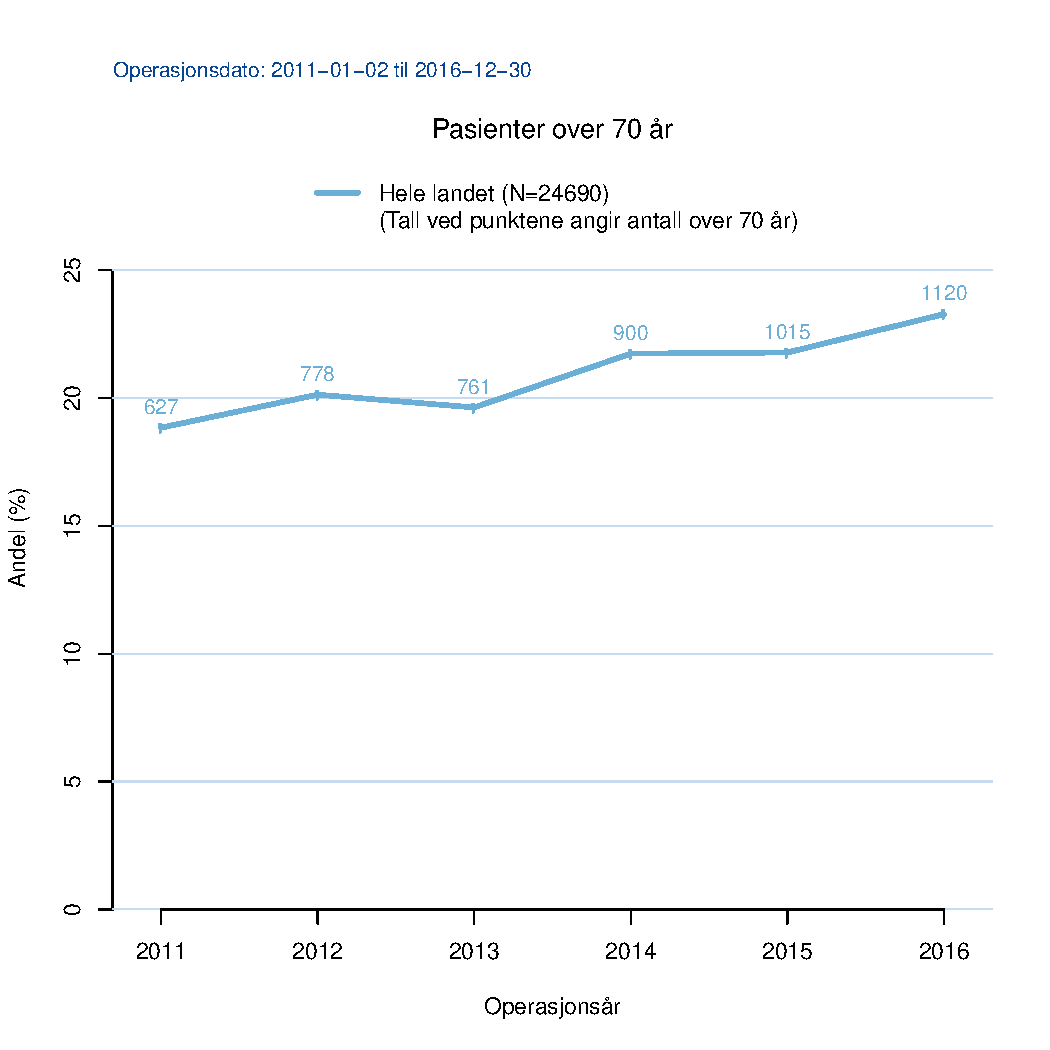
\includegraphics{Figurer/FigAlder70.pdf}}
\caption{\label{fig:Alder70} Andel ryggoperasjoner utført på personer som er 70 år eller mer.}}
\end{figure}



%Figur \ref{fig:Alder} viser aldersfordeling for alle pasienter i rappAar.

%\begin{figure}[ht]
%	\centering 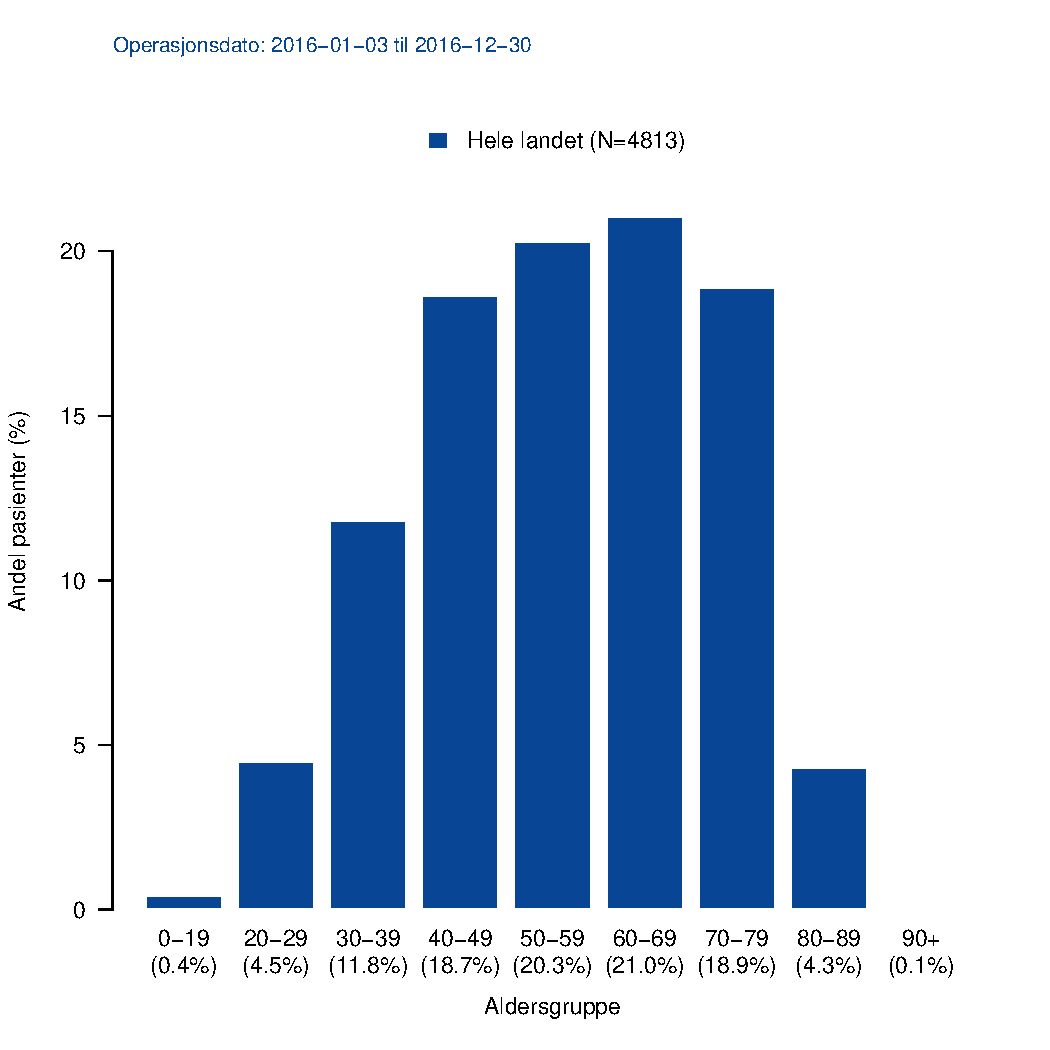
\includegraphics[width= s1\textwidth]{FigAlderFord.pdf}
%	\caption{\label{fig:Alder} paste0(AlderFord$Tittel,', ',rappAar)}
%\end{figure}

\subsection{Kroppsmasseindex (Body Mass Index, BMI)}



Opplysninger om høyde og vekt er rapportert fra pasientene selv.
Andelen pasienter med fedme har vært jevt økende fra NA \% 
i 2011
til 25.6 \%
i  2017.

Publikasjoner fra NKR viser at pasienter med fedme kan forvente signifikant mindre bedring etter 
ryggkirurgi sammenliknet med de som har lavere BMI. 




\subsection{Morsmål / etnisitet og utdanning}



Andelen fremmedspråklige (inkl. samisk) som opereres har økt fra 4.6 \% til 6.9 \% i perioden 2011 til 2017.\\
Beslutning om ryggkirurgi baserer seg på en felles forståelse mellom kirurg og
pasient av hva helseproblemene består i og hva som kan oppnås med operasjon
(«shared desicion making»). I behandling av fremmedspråklige er kommunikasjon
en utfordring. Eksempelvis var suksessraten ved lumbal prolapskirurgi for de med norsk som morsmål 65 \% mot 56 \% \it{Tore sjekk tall} 
for fremmedspråklige. Bedre kommunikasjon kan bidra å redusere disse
forskjellene. Figur \ref{fig:Morsmal} viser andelen fremmedspråklige operert ved de ulike avdelingene i 2017.

\begin{figure}[ht]
\scalebox{0.7}{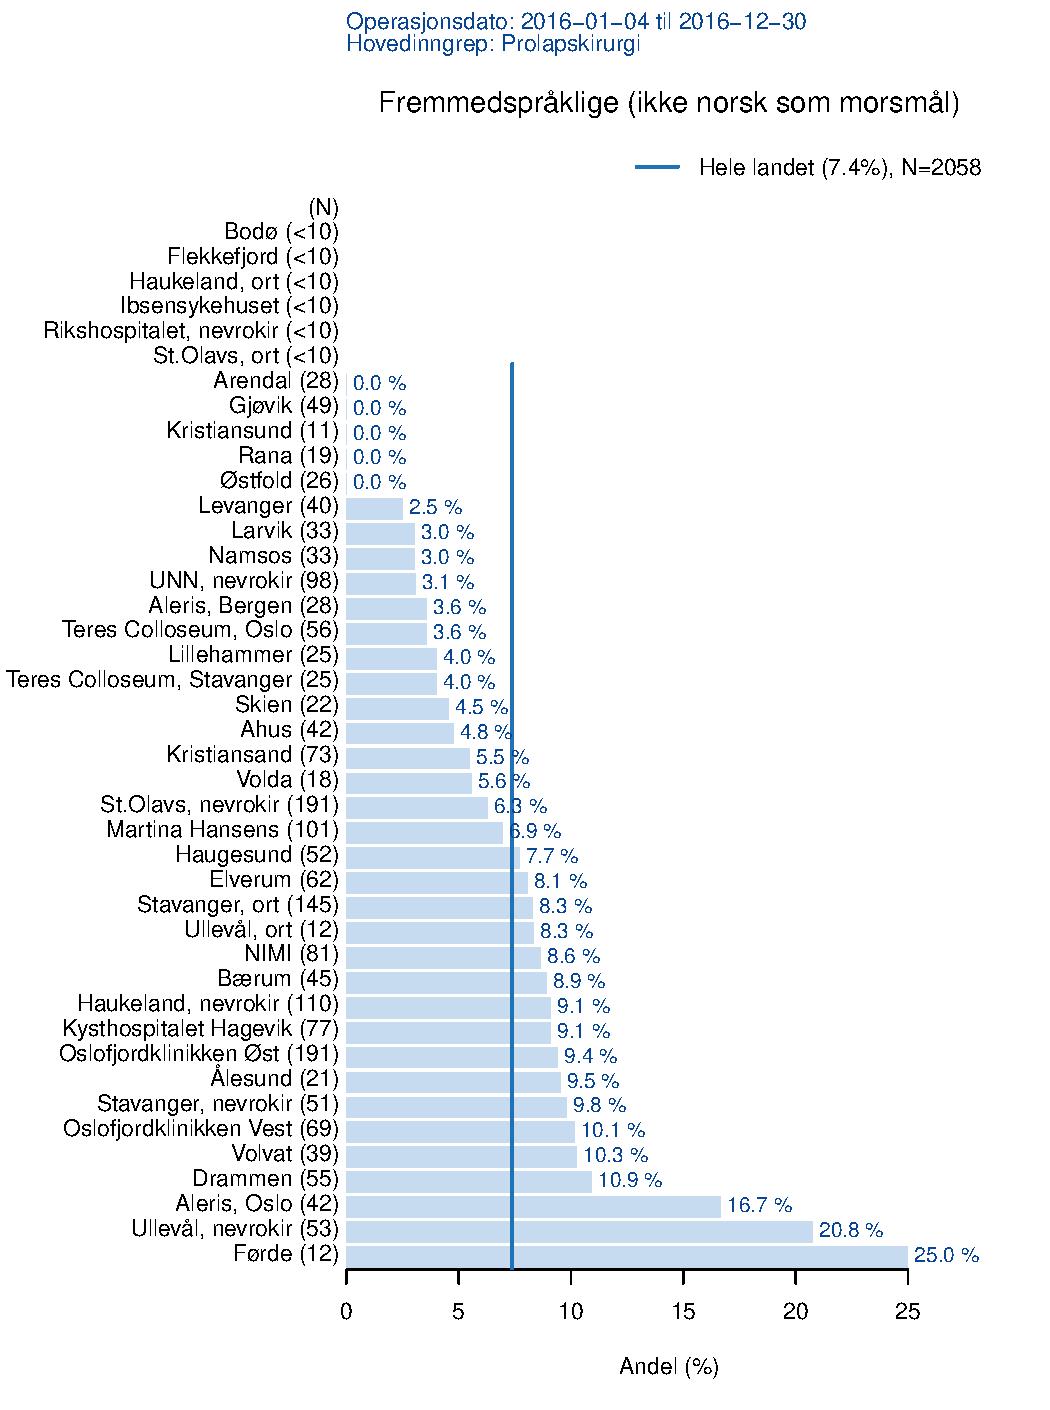
\includegraphics{Figurer/FigMorsmal.pdf}}
\caption{\label{fig:Morsmal} Andel fremmedspråklige av alle ryggopererte ved ulike sykehus i
Norge.}
\end{figure}




Lav utdanning er assosiert til dårligere operasjonsresultat. Andelen ryggopererte med høyere utdanning (høyskole eller universitet) var 36.6 i 2017 mot  30.9 i 2011. 
Opplysningene om utdanning er rapportert av pasientene selv. 
Figur \ref{fig:HoyUtdAvd} viser andel ryggopererte 
med høyskole eller universitetsutdanning ved hvert sykehus/avdeling.


\begin{figure}[ht]
\scalebox{0.7}{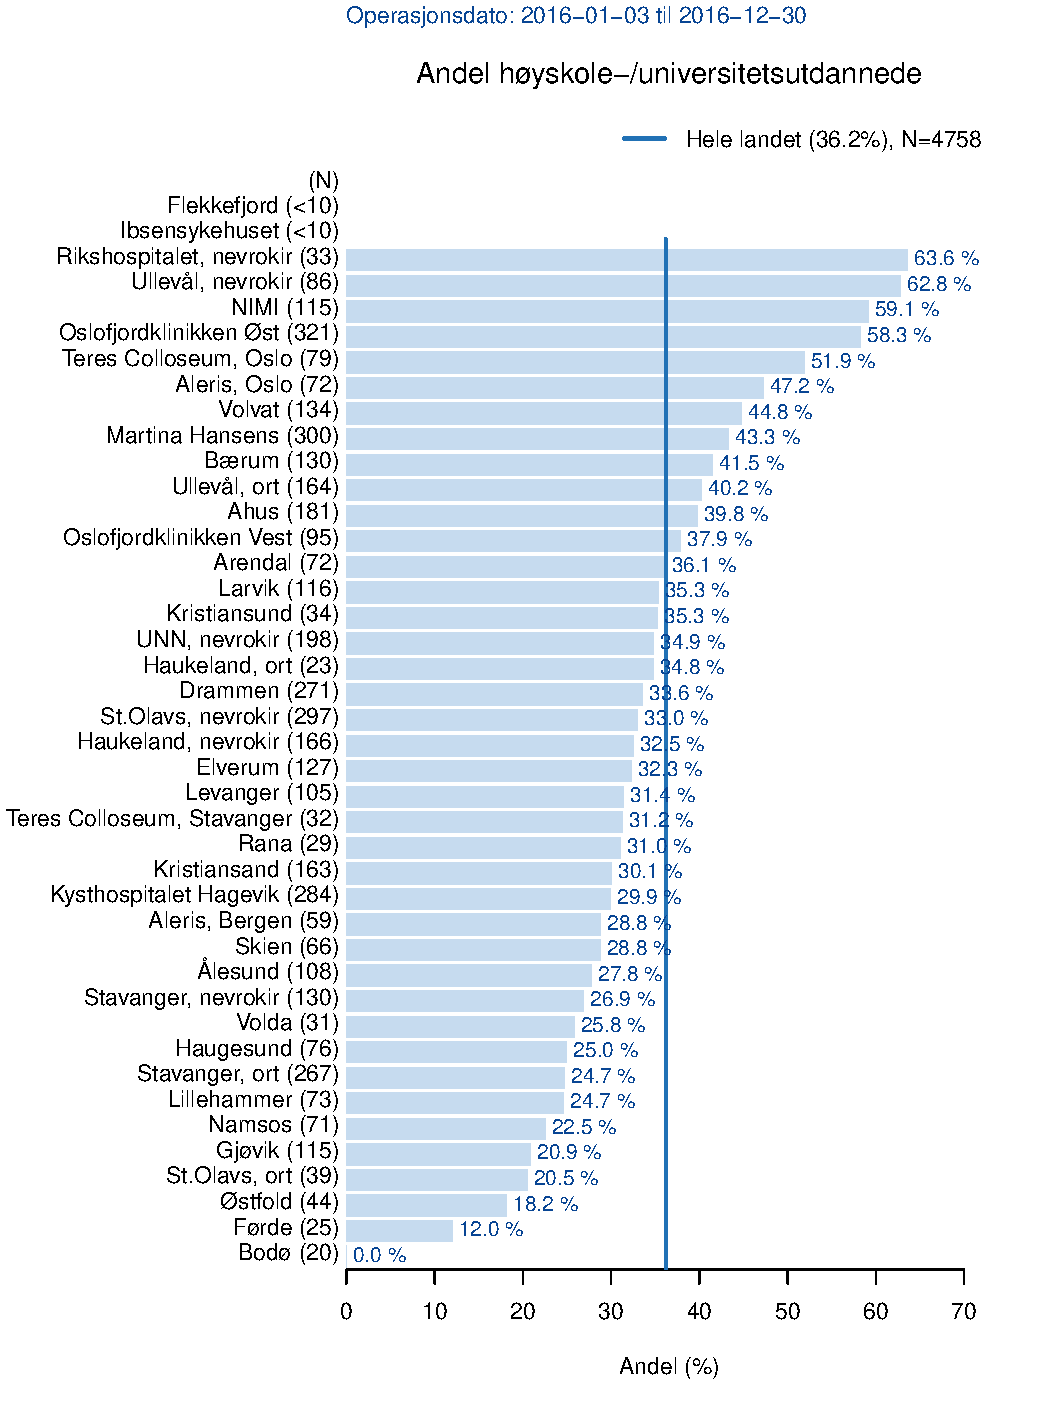
\includegraphics{Figurer/FigHoyUtdAvd.pdf}}
\caption{\label{fig:HoyUtdAvd} Andel pasienter med høyere utdanning (høyskole/universitet).}
\end{figure}


\clearpage

\subsection{Arbeidsstatus}

% latex table generated in R 3.5.0 by xtable 1.8-2 package
% Wed Sep 12 15:11:31 2018
\begin{table}[ht]
\centering
\begin{tabular}{lr}
  \hline
 & Andeler \\ 
  \hline
I arbeid & 19.8\% \\ 
  Hjemmeværende & 1.3\% \\ 
  Student/skoleelev & 1.3\% \\ 
  Pensjonist & 31.1\% \\ 
  Arbeidsledig & 1.5\% \\ 
  Sykemeldt & 20.6\% \\ 
  Aktiv sykemeldt & 0.9\% \\ 
  Delvis Sykemeldt & 7\% \\ 
  Attføring/rehabiliteirng & 4.2\% \\ 
  Uføretrygdet & 12.3\% \\ 
   \hline
\end{tabular}
\caption{Arbeidsstatus, pasienter operert i 2017} 
\label{tab:Arb}
\end{table}


Tabell \ref{tab:Arb} viser fordeling av arbeidsstatus før operasjon for de 98.5\% 
av pasientene i registeret som har svart på spørsmål om arbeidsstatus. 
Andelen pasienter som mottok sykepenger (sykemeldte, uføretrygdede eller personer 
på attføring) og av den grunn var helt eller delvis ute av jobb før operasjonen var 
45 \%. 

%\clearpage


\subsection{Uføretrygd og erstatning }




Pasienter som har en uavklart uføre eller erstatningssak vil sjeldnere komme tidlig tilbake i jobb etter operasjon.
Både andel som har søkt eller planlegger å søke uføretrygd eller erstatning ligger stabilt og var i 2017 
henholdsvis 4.7 og 4.5. 
Figur \ref{fig:Ufor} viser andel ryggopererte ved hver avdeling som har søkt eller planlegger å søke uføretrygd.

\begin{figure}[ht]
\scalebox{0.7}{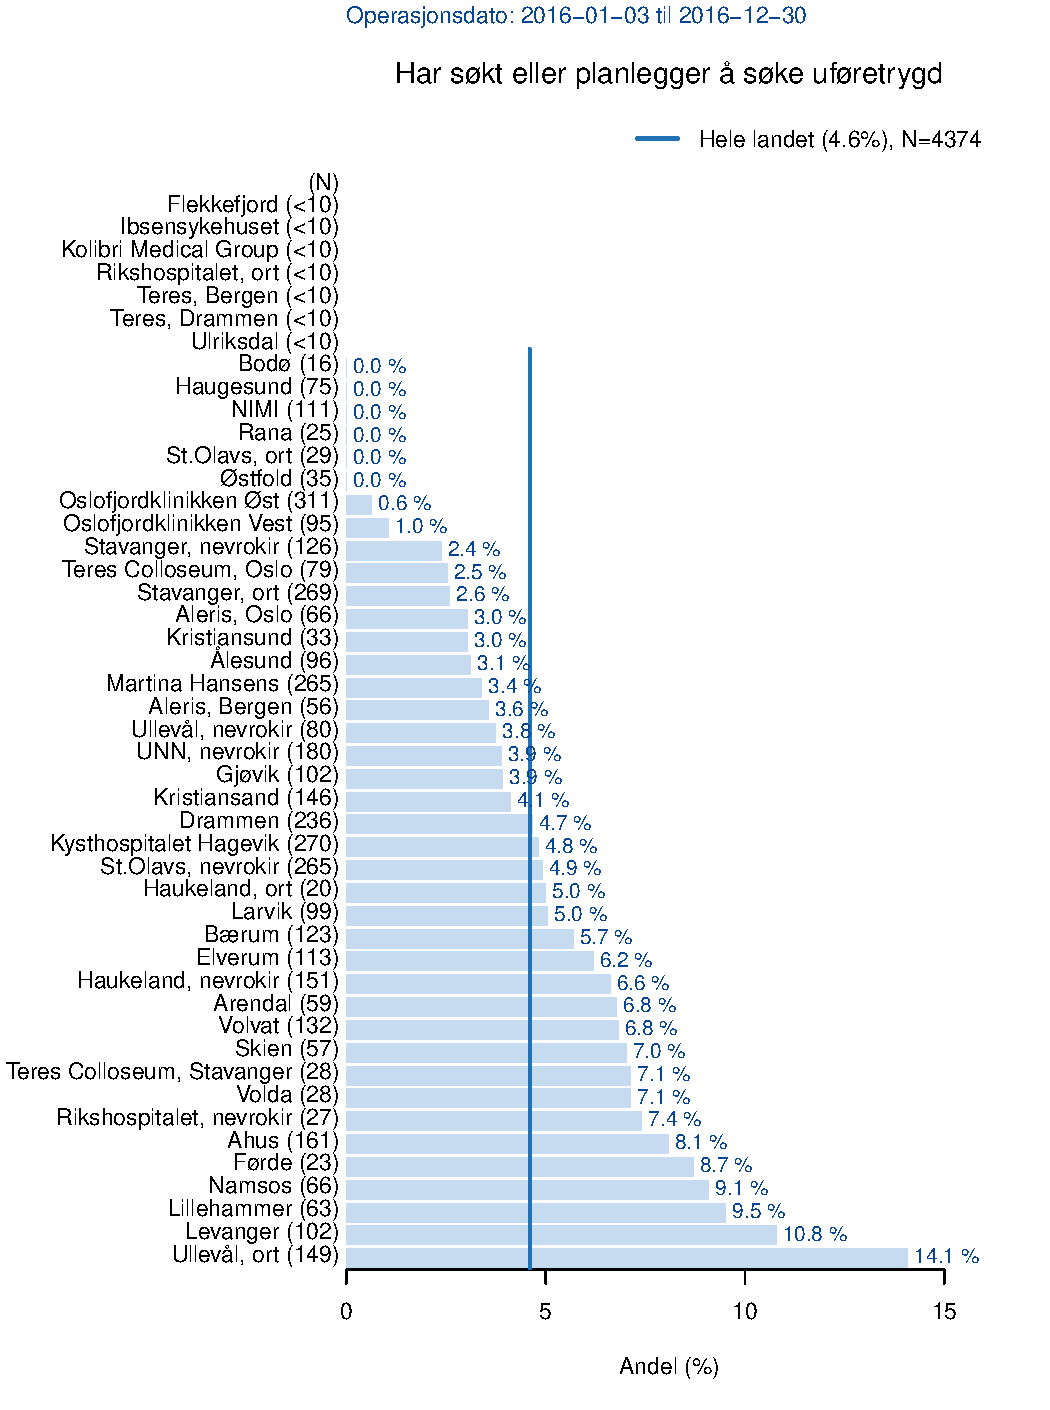
\includegraphics{Figurer/FigUforAvd.pdf}}
\caption{\label{fig:Ufor} Andel pasienter som har søkt eller planlegger å søke uføretrygd} 
\end{figure}


\clearpage

\subsection{Tidligere ryggoperert}
Informasjonen er hentet fra legeskjema.
%Figur \ref{fig:TidlOp} viser en prosentvis fordelig mellom primæroperasjon, det vil si første gangs 
%operasjon, og operasjoner hos pasienter som har vært operert tidligere.  
%Søylene representerer hvert år frem til i dag. Tallet på toppen av søylen viser antall operasjoner utført 
%det aktuelle året. 
Reoperasjon gir genereltl dårligere operasjonsresultat enn første gangs operasjon.





Andelen reoperasjoner var 25 \% i 2011 og 27 \% i 2017.
Av de pasientene operert i 2017 som hadde vært operert tidligere, var 57.6\% 
operert i samme nivå, 33.7\% 
operert i annet nivå og 8.6\% 
operert i både samme og annet nivå.




NKR har tidligere vist at multiple reoperasjoner har minimal effekt. Andelen som har vært operert 
mer enn 2 ganger tidligere ligger mellom 0.9 \%
og 1.6 \% for prolapspasienter og mellom 1.7 \%
og 3.1 \% for spinal stenosepasienter i perioden 2011-2017. 



\subsection{ASA-grad og røyking}
ASA angir pasientens ”sårbarhet” i forhold til å få anestesi og operasjon på en skala fra 1 til 5. 
Opplysningene hentes fra legeskjema.
% latex table generated in R 3.5.0 by xtable 1.8-2 package
% Wed Sep 12 15:11:36 2018
\begin{table}[ht]
\centering
\begin{tabular}{crr}
  \hline
 & Antall & Prosent \\ 
  \hline
I & 1362 & 25.8\% \\ 
  II & 3090 & 58.6\% \\ 
  III & 784 & 14.9\% \\ 
  IV & 10 & 0.2\% \\ 
  V & 1 & 0\% \\ 
  Ikke besvart & 25 & 0.5\% \\ 
   \hline
\end{tabular}
\caption{Fordeling av ASA-grad, operasjoner utført i 2017} 
\label{tab:ASA}
\end{table}


Tabell \ref{tab:ASA} viser fordeling av ASA grad. Andelen pasienter med ASA grad I-II 
var 84.4\%. Pasienter som røyker, havner 
automatisk i ASA-grad II eller høyere. 
%txt
Andel røykere har gått fra 28.2 i 2011 til 19.1 i 2017.



\subsection{Radiologisk utredning}

% latex table generated in R 3.5.0 by xtable 1.8-2 package
% Wed Sep 12 15:11:38 2018
\begin{table}[ht]
\centering
\begin{tabular}{lrr}
  \hline
 & Antall & Andeler \\ 
  \hline
CT & 371 & 7\% \\ 
  MR & 5175 & 98\% \\ 
  Radikulografi & 38 & 1\% \\ 
  Diskografi & 2 & 0\% \\ 
  Diagnostisk blokade & 28 & 1\% \\ 
  Røntgen LS-columna & 1208 & 23\% \\ 
  Med fleksjon/ekstensjon & 394 & 7\% \\ 
  Tot. ant. & 5272 &   \\ 
   \hline
\end{tabular}
\caption{Radiologisk vurdering, 2017} 
\label{tab:RV}
\end{table}


Tabell \ref{tab:RV} viser hvor stor andel av pasientene som har vært til ulike typer 
radiologisk undersøkelse. En pasient kan ha vært til flere undersøkelser. Hyppigste radilologiske diagnoser er skiveprolaps og spinal stenose.
Spørsmålene er besvart av leger. 




% latex table generated in R 3.5.0 by xtable 1.8-2 package
% Wed Sep 12 15:11:38 2018
\begin{table}[ht]
\centering
\begin{tabular}{lrr}
  \hline
 & Antall & Andeler \\ 
  \hline
Skiveprolaps & 2346 & 44\% \\ 
  Sentral spinalstenose & 1755 & 33\% \\ 
  Lateral spinalstenose & 1771 & 34\% \\ 
  Foraminal stenose & 636 & 12\% \\ 
  Degenerativ rygg/skivedegenerasjon & 926 & 18\% \\ 
  Istmisk spondylolistese & 143 & 3\% \\ 
  Degenerativ spondylolistese & 521 & 10\% \\ 
  Degenerativ skoliose & 155 & 3\% \\ 
  Synovial syste & 144 & 3\% \\ 
  Pseudomeningocele & 1 & 0\% \\ 
  Tot.ant. & 5272 &   \\ 
   \hline
\end{tabular}
\caption{Radiologiske diagnoser, 2017} 
\label{tab:RF}
\end{table}


Tabell \ref{tab:RF} viser diagnoser basert på radiologiske funn hos alle pasienter 
i 2017. 
Spørsmålene er besvart av leger.
En pasient kan ha flere diagnoser/radiologiske funn.
%txtRFnorm




\section{Virksomhetsdata}

Andelen som er operert ved hjelp av synsfremmende midler (mikroskop eller
lupebriller), som har åpenbare fordeler, har økt fra 86 \% i 2011 til 
98 \% i 2017 for prolapsoperasjoner. 
For spinal stenose er endringa fra 68 \% i 2011 til 
98 \% i 2017.



\subsection{Type operasjon}



De hyppigste tilstandene pasienter ble operert for i 2017 var prolapskirurgi (41 \%) og spinal stenose (42 \%). Tabell \ref{tab:AntHovedInngrep} viser fordeling av hovedinngrepstype, samt antall registrerte operasjoner for hver hovedinngrepstype.
''Foramenotomi'' betyr at det er gjort dekompresjon for spinal stenose med bevaring av midtlinjestrukturer.

% latex table generated in R 3.5.0 by xtable 1.8-2 package
% Wed Sep 12 15:11:38 2018
\begin{table}[ht]
\centering
\begin{tabular}{lrr}
  \hline
 & Antall & Andeler \\ 
  \hline
Udefinerbart & 161 & 3\% \\ 
  Prolapskirurgi & 2161 & 41\% \\ 
  Foramenotomi & 2087 & 40\% \\ 
  Laminektomi & 191 & 4\% \\ 
  Interspin. implantat & 1 & 0\% \\ 
  Fusjonskirurgi & 598 & 11\% \\ 
  Skiveprotese & 45 & 1\% \\ 
  Rev. av implantat & 28 & 1\% \\ 
   \hline
\end{tabular}
\caption{Fordeling av hovedinngrep, 2017} 
\label{tab:AntHovedInngrep}
\end{table}



%\begin{figure}[ht]
%      \scalebox{s1}{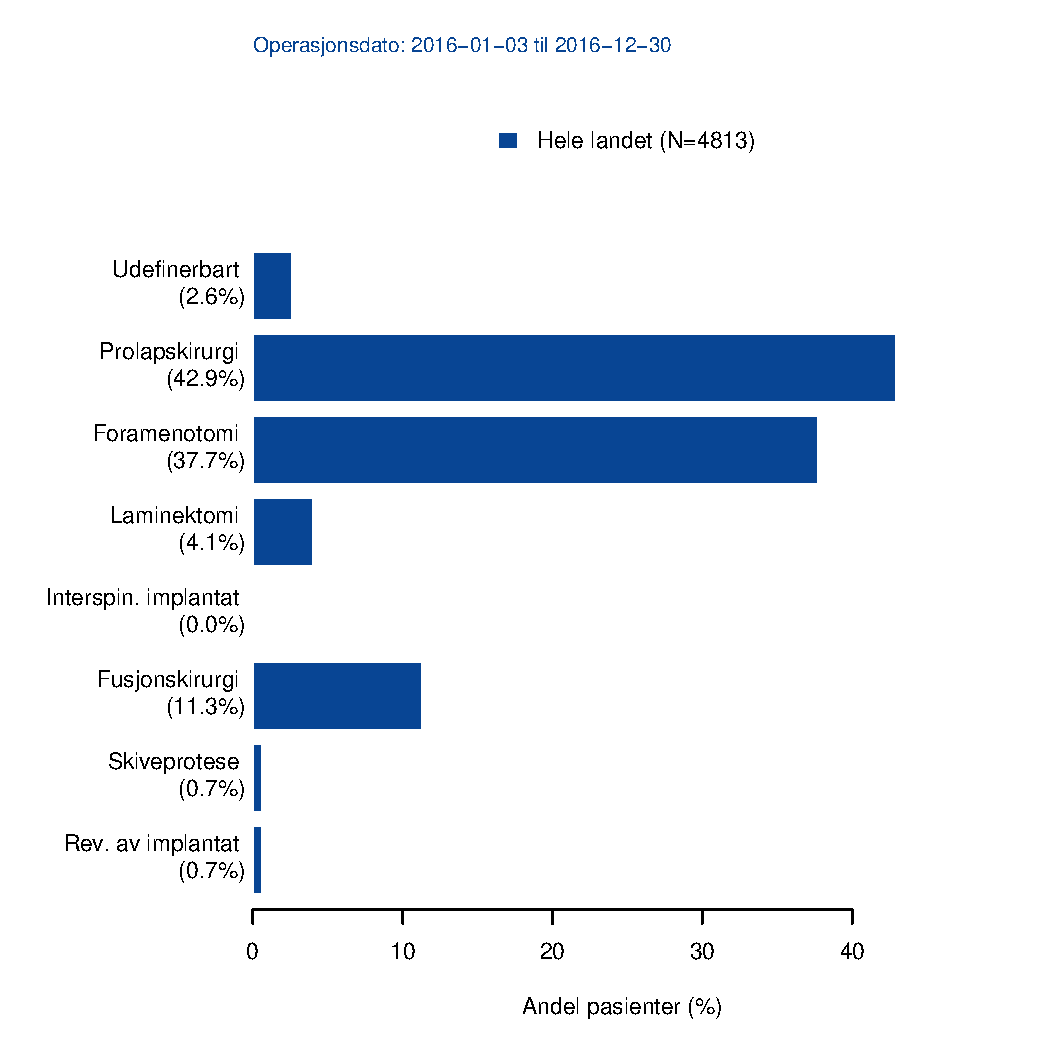
\includegraphics{Figurer/HovedInngrep.pdf}}
%      \caption{\label{fig:HovedInngrep} HovedInngrep$Tittel}
%\end{figure}



\subsubsection{Degen. spondylolistese operert med fusjonskirurgi}


 LENA:

XX \% av de som ble operert for spinal stenose i 2017 hadde også en forskyvning mellom ryggvirvlene (Degenerativ spondylolistese). I faglitteraturen er det sprikende anbefalinger for om denne undergruppen skal ha tilleggsbehandling med avstivningsoperasjon (fusjonskirurgi).
Figur \ref{fig:degSponFusj} viser at det er stor variasjon i bruk av denne fusjonskirurgi, 
for denne pasientgruppen i Norge, også mellom avdelinger på samme sykehus. 

Norske studier baser på data fra NKR har vist at tilleggseffekten er liten og assosiert til høyere kostnader. 
I 2018 blir det publisert en studie baser på data fra NKR, og tilsvarende registre i Sverige og Danmark (SWEspine og DANEspine). Denne viser  at tilleggbehandling med fusjonskirurgi ikke er assosiert til større behandlingseffektivitet, men lengre liggetid på sykehus. En pågående nasjonal RCT studie skal se nærmere på dette. Denne studien vil blant annet kunne svare på om undergrupper av pasienter med spinal stenose og degenerativ spondylolistese kan ha nytte av fusjonskirurgi.


Figur...(Ny figur: andel pasienter med degenerativ spondylolistese og spinal stenose som blir operert med fusjonskirurgi per år.) viser at andelen spinal stenoseopererte som får tilleggsbehandling med fusjonskirurgi er redusert fra ..\% i 2011 til ...\% i 2017.
\textit{LENA: AndelTid}

\begin{figure}[ht]
\scalebox{0.7}{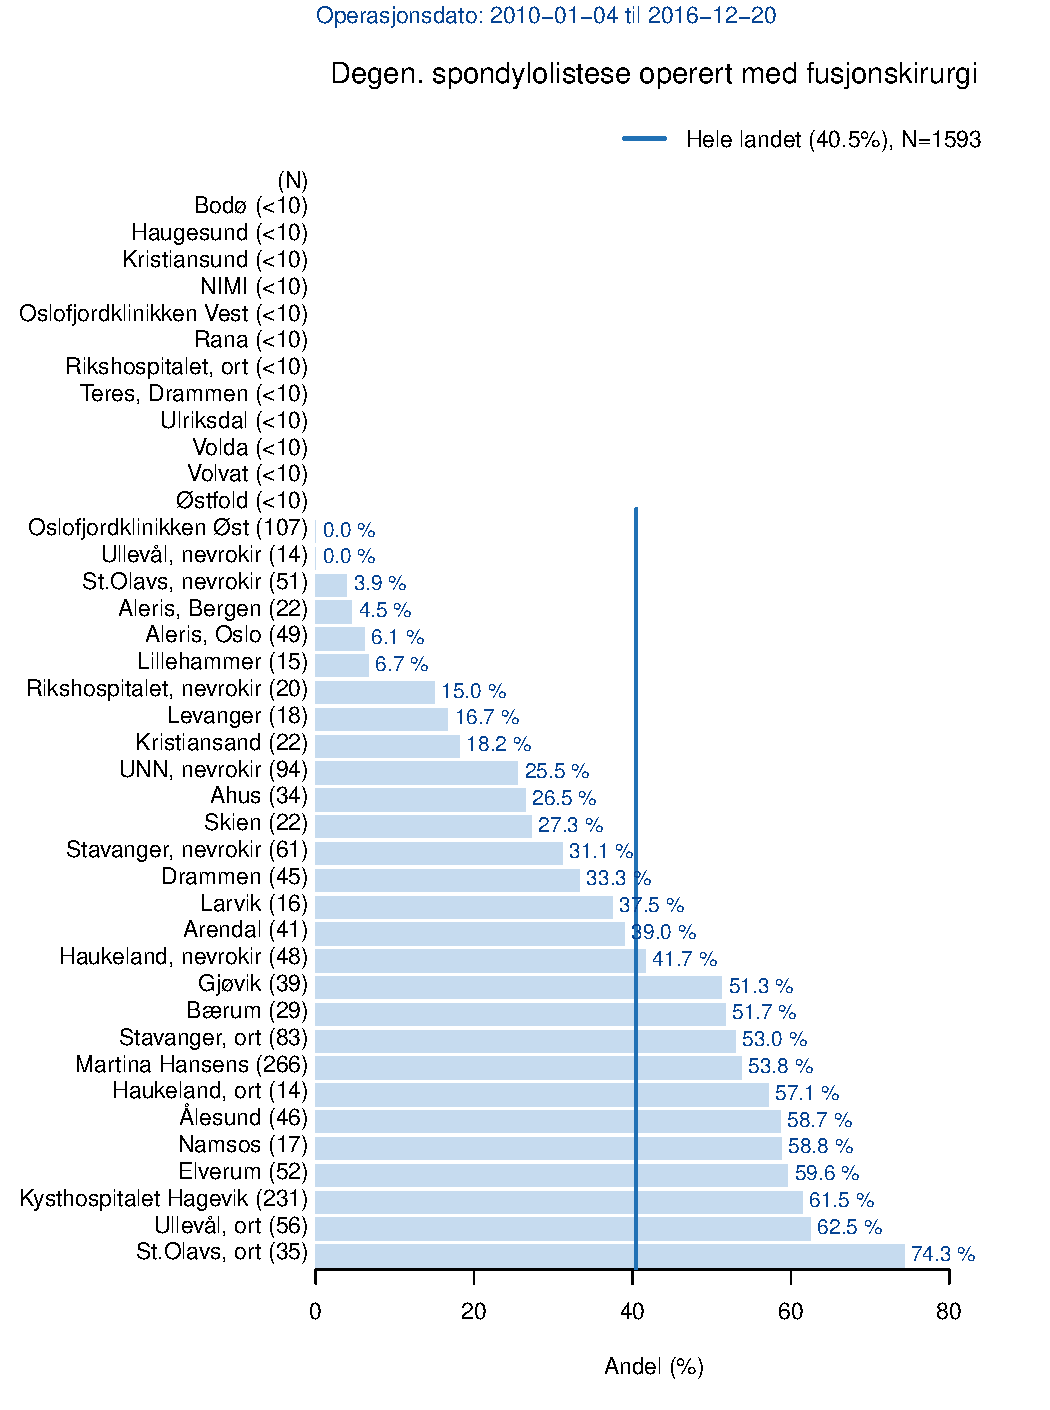
\includegraphics{Figurer/FigdegSponFusj.pdf}}
\caption{\label{fig:degSponFusj} Degenerativ spondylolistese operert med fusjonskirurgi}
\end{figure}

Nevrokirurgiske avdelinger fikserer lite sammenliknet med ortopeder.

\clearpage

\subsection{Liggetid}

Informasjonen er hentet fra legeskjema.
%Figur \ref{fig:Liggedogn} viser liggedøgnsfordeling for alle pasienter operert i rappAar. 
%Figur \ref{fig:LiggedognTid} viser gjennomsnittlig antall liggedøgn per år.  
Det har vært en klar reduksjon i liggetid  på sykehus (ca 1 døgn) fram til 2017 for både lumbal prolaps og spinal stenose opererte. Figur \ref{fig:LiggetidAvdPro} og \ref{fig:LiggetidAvdSS} viser at det er stor variasjon i antall liggedøgn mellom sykehus og avdelinger.
Dette kan henge sammen med økt bruk av mindre invasive operasjonsmetoder og mer dagkirurgi. 





%\begin{figure}[h] 
%\scalebox{s1}{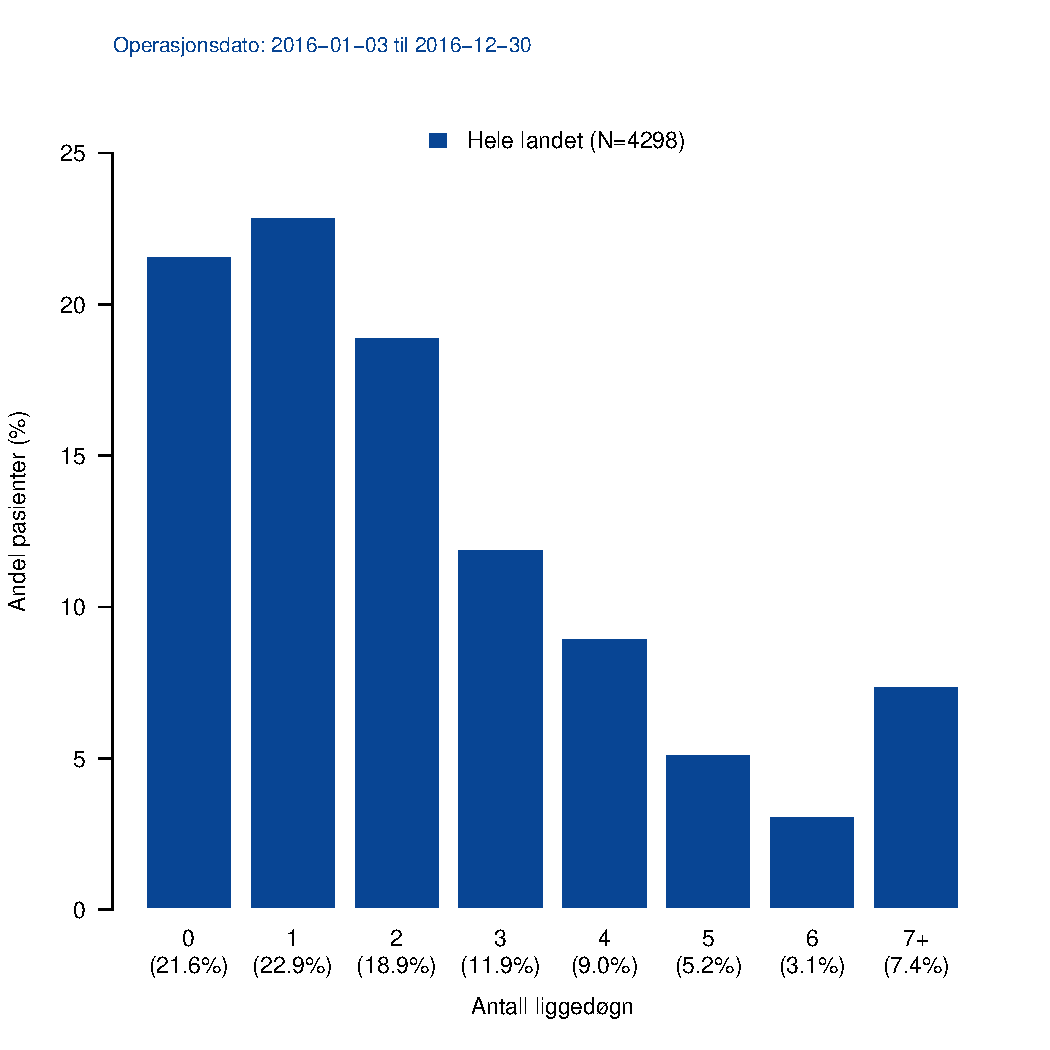
\includegraphics{Figurer/FigLiggetidFord.pdf}}
%\caption{LiggetidFord$Tittel}
%\label{fig:Liggedogn}
%\end{figure}

% \begin{figure}[h] 
% \centerline{
% \scalebox{s2}{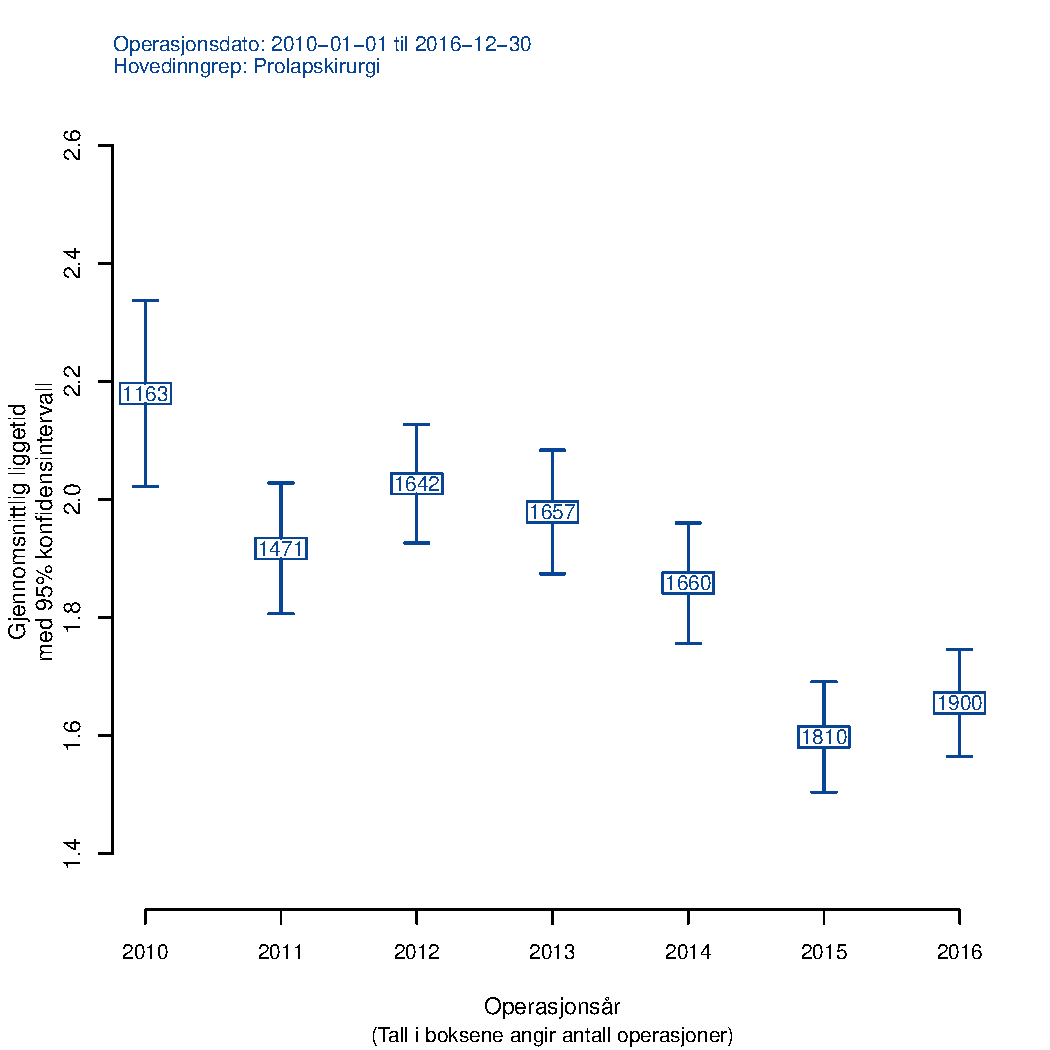
\includegraphics{Figurer/LiggetidBoxPro.pdf}}
% \scalebox{s2}{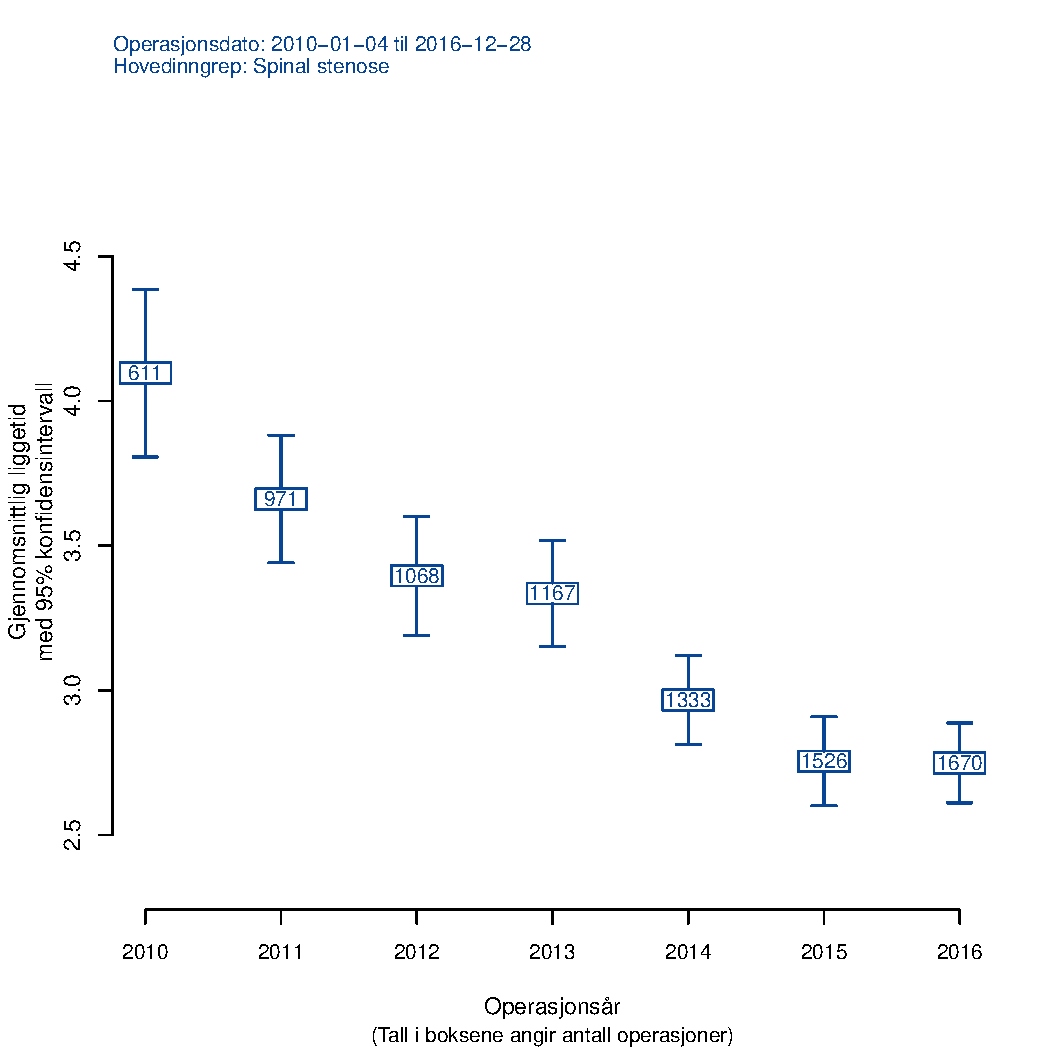
\includegraphics{Figurer/LiggetidBoxSS.pdf}}
% }
% \caption{Gjennomsnittlig liggetid for hhv. prolaps og spinal stenose. }
% \label{fig:LiggedognTid}
% \end{figure}

\begin{figure}[h] 
\scalebox{0.7}{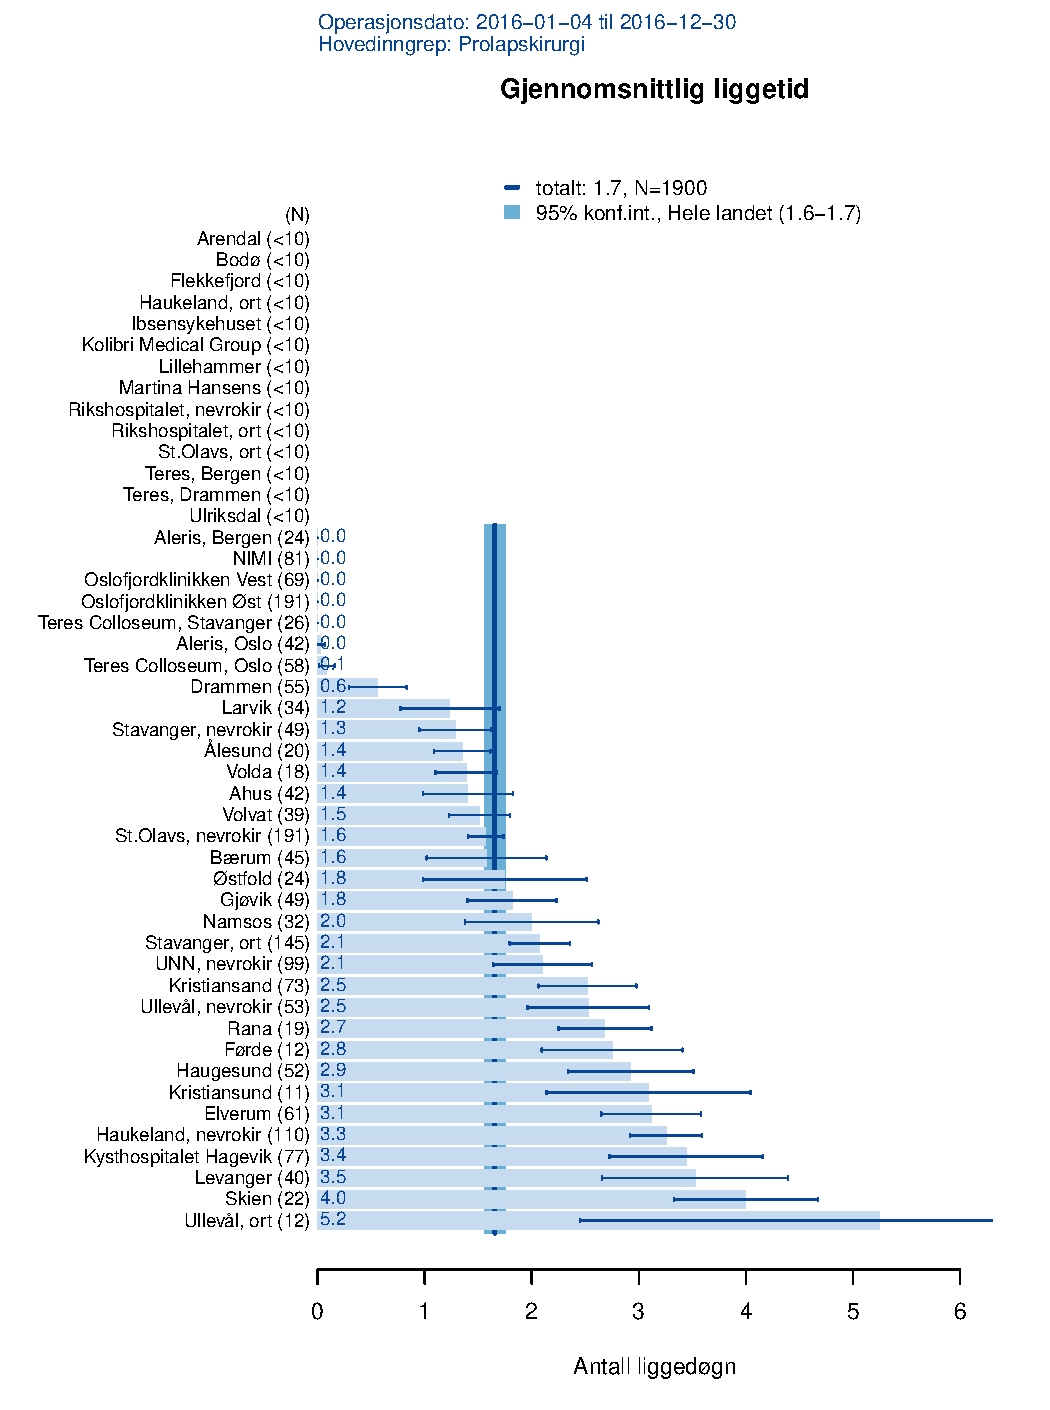
\includegraphics{Figurer/LiggetidAvdPro.pdf}}
\caption{Gjennomsnittlig liggetid for lumbalt prolaps ved ulike avdelinger. Noen sykehus har mest dagkirurgi og får derfor få observasjoner. } 
\label{fig:LiggetidAvdPro}
\end{figure}

\begin{figure}[h] 
\scalebox{0.7}{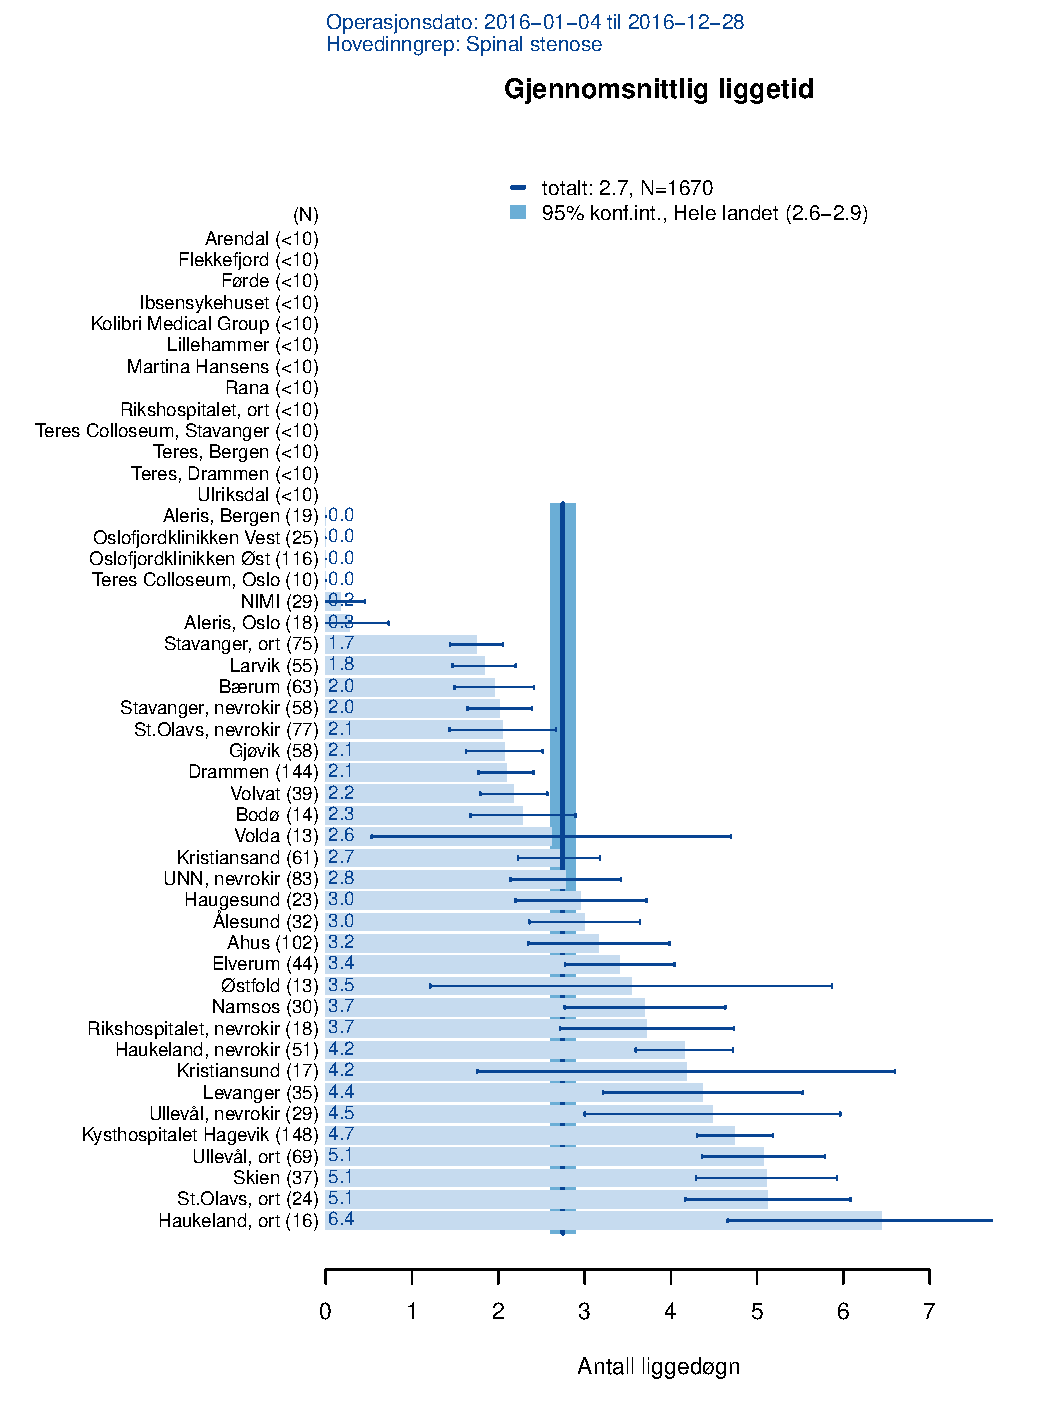
\includegraphics{Figurer/LiggetidAvdSS.pdf}}
\caption{Gjennomsnittlig liggetid for spinal stenose ved ulike avdelinger. Noen sykehus har mest dagkirurgi og får derfor få observasjoner. } 
\label{fig:LiggetidAvdSS}
\end{figure}






\clearpage

\section{Resultatmål}
All informasjon i dette kapitlet er hentet fra pasientskjema. Ingen av resultatmålene er justert
for eventuelle ulikheter i pasientpopulasjonene. Noen viktige forskjeller som kan forklare en del av forskjeller i resultat er vist i de forgående kapitlene.
Resultatmålene er utviklet gjennom forskning (valideringsstudier) i regi av NKR og i samarbeid
med blant annet Nasjonalt kompetansesenter for rygg og nakke kirurgi. Noen fra er hentet fra annen
internasjonal forskning. De terskelverdiene som brukes er med andre ord forskningsbaserte. 
Det er viktig å merke seg at pasienter som er operert i 2016 først får resultater fra ettårs oppfølgning i 2017. 

Viktige årsaker til variasjon i operasjonsresultat kan være at sykehusene behandler
ulike pasientgrupper. Viktig for operasjonsresultatet er imidlertid fortsatt
indikasjonsstillingen («inngangsbilletten») til kirurgi; Fikk riktig person, rett
behandling til rett tid?

Forekomst av risikofaktorer blant pasientene påvirker operasjonsresultatene og kan
si noe om hvor godt behandlingstilbudet fungerer på ulike sykehus. Noen av disse
faktorene kan modifiseres/bedres gjennom bedre styring og planlegging av
virksomheten, strengere indikasjonsstilling og bedret pasientsikkerhet.




\subsection{ Resultater etter ryggkirurgi, 2011 til 2017}

\subsection{Oswestry Disability Index (ODI)}





ODI brukes som hovedeffektmål og uttrykker smerterelatert fysisk funksjon og sykdomsspesifikk livskvalitet hos ryggpasienter. Skalaen går fra 0
til 100, hvor 0 angir ingen funksjonshemming og følgelig beste livskvalitet.
Pasienten angir smerteintensitet i henholdsvis ben og rygg på en numerisk smerteskala (NRS), 
fra 0 (ingen smerte) til 10 (verst tenkelige smerte).
\\

Gjennomsnittlig ODI score var 46.4 før operasjon og 16.7 ett år etter
operasjon for lumbalt prolapsopererte i 2016. Dette betyr at funksjonssvikten ble redusert 
fra alvorlig til minimal for gjennomsnittspasienten. \\

Pasienter operert for spinal stenose fikk også
betydelig bedring (ODI redusert fra 39.2 til 23.2), men mange har 
fortsatt lett til moderat funksjonssvikt ett år etter kirurgi. 
De som ble operert med fusjon har
omtrent samme forbedring (ODI redusert fra 42.0 til 25.1). 
Dette betyr at selv om
pasientene kan forvente en betydelig bedring, vil mange fortsatt ha en del restplager
ett år etter kirurgi. 
Resultatene synes å være omtrent de samme fra år til år. NKR
sammenstiller også norske resultater med data fra tilsvarende registre i Sverige og
Danmark, og resultatene synes å være de samme i de tre nordiske landene.
Resultatene varierer imidlertid mye mellom sykehus og fra pasient til pasient.


%Figur \ref{fig:OswEndr} viser gjennomsnittlig endring av ODI fra før operasjon til ett år etter.
endring av funksjon i dagliglivet og sykdomsspesifik livskvalitet
Merk at resultatene \textit{ikke} er justert for forskjeller i pasientpopulasjonene. 




Figurene \ref{fig:OswEndrAvdPro} og \ref{fig:OswEndrAvdSS} viser gjennomsnittlig endring 12 måneder etter for hver avdeling for henholdsvis prolaps og spinal stenose pasienter. Forskjellene er små. Vi ser også at konfidensintervallene er relativt brede og overlappende.

\begin{figure}[h] 
\scalebox{0.7}{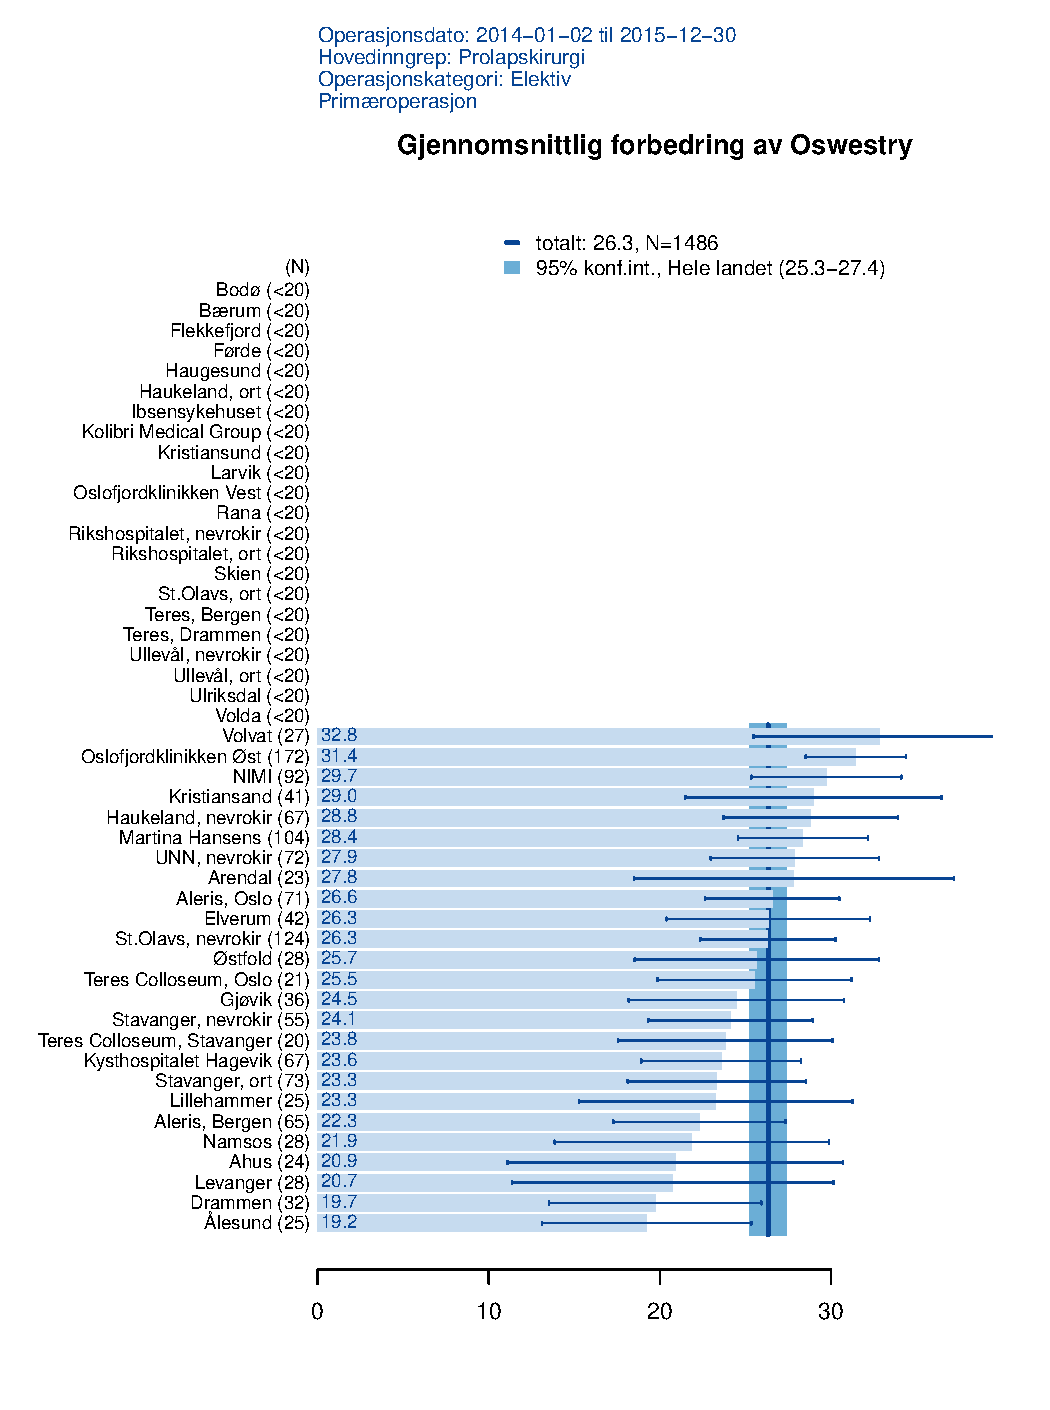
\includegraphics{Figurer/OswEndrAvdPro.pdf}}
\caption{Gjennomsnittlig endring av ODI per avdeling for lumbalt prolaps.}
\label{fig:OswEndrAvdPro}
\end{figure}

\begin{figure}[h] 
\scalebox{0.7}{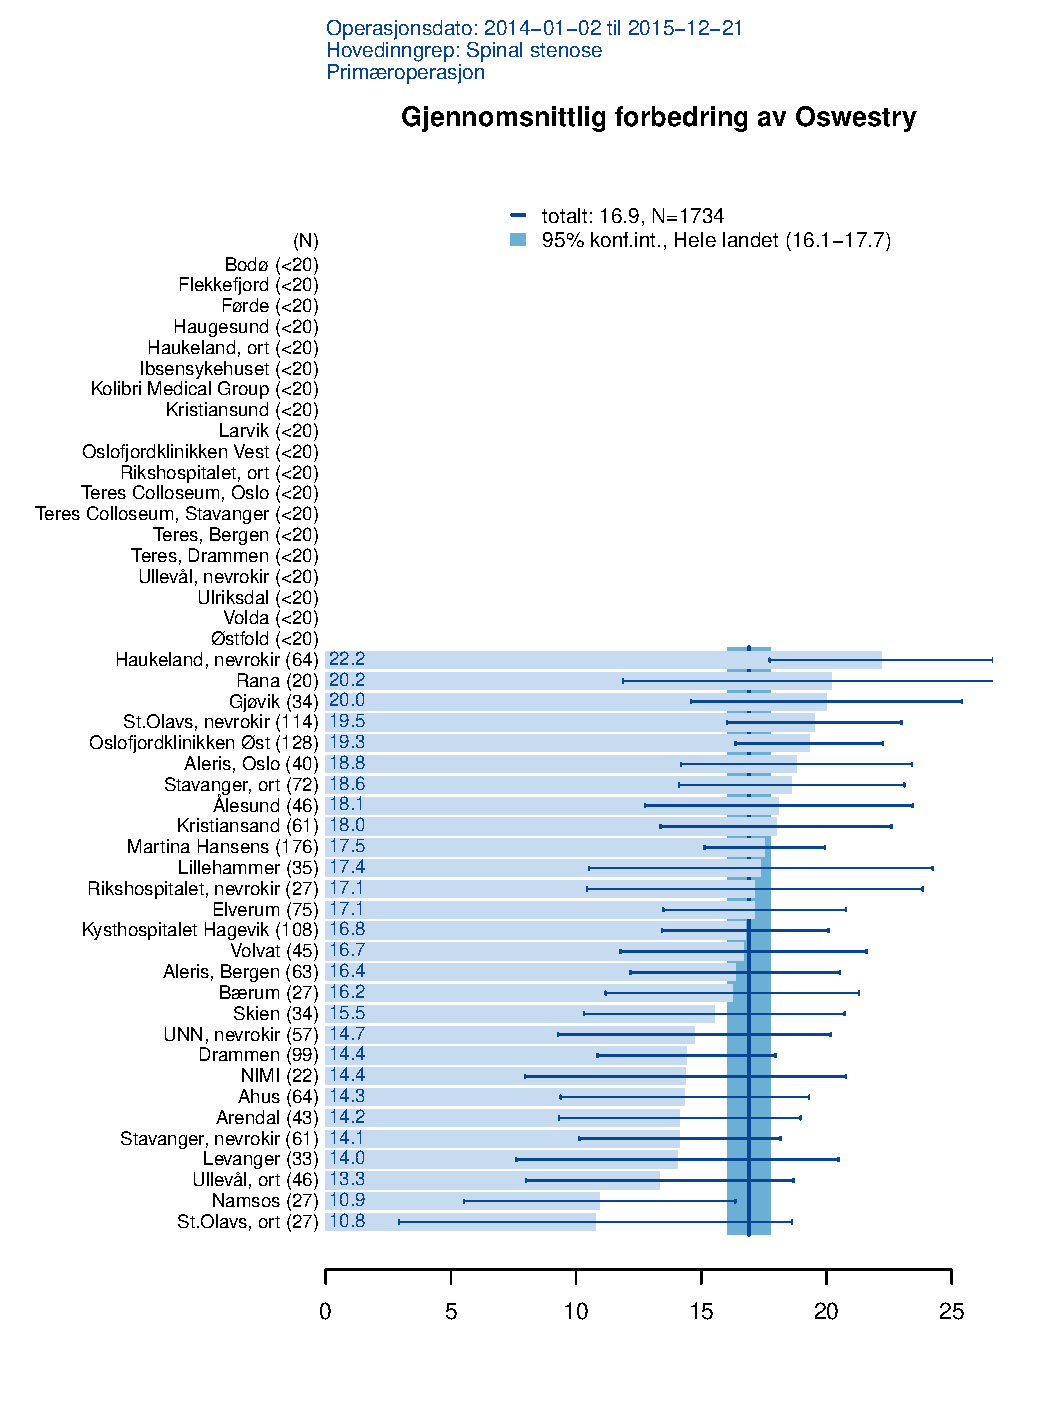
\includegraphics{Figurer/OswEndrAvdSS.pdf}}
\caption{Gjennomsnittlig endring av ODI per avdeling for spinal stenose.}
\label{fig:OswEndrAvdSS}
\end{figure}




Suksessrate, det vil si forbedring i Oswestry på mer enn 20 poeng, ligger stabilt rundt 60 \% for prolapspasienter, ett år etter operasjon. 
For spinal stenosepasienter er "suksess" forbedring i Oswestry på mer enn 30 \% , ett år etter operasjon. Denne raten ligger også stabilt rundt 60\%.


\clearpage

ODI skår  under 22 poeng oppleves av de fleste pasientene som et helt akseptabelt fysisk funksjonsnivå 12 mnd etter ryggopersjon. Figurene \ref{fig:Osw22Pro} og \ref{fig:Osw22SS} angir hvor stor andel av henholdsvis prolaps og spinal stenose opererete som oppnår dette.

\begin{figure}[ht]
\scalebox{0.7}{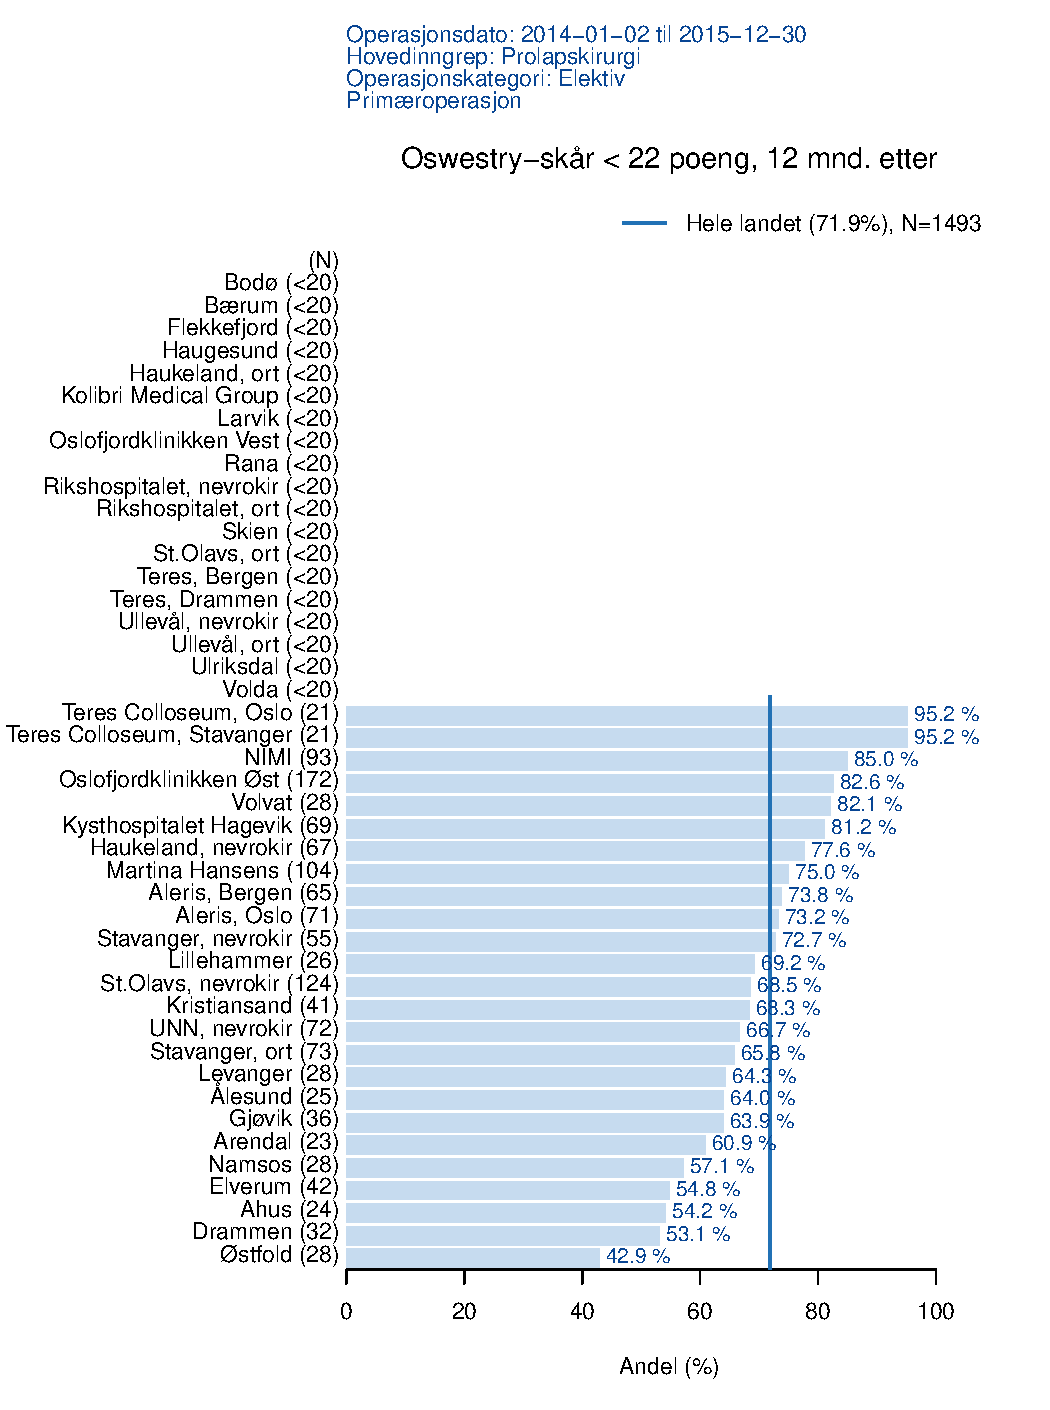
\includegraphics{Figurer/FigOsw22Pro.pdf}}
\caption{\label{fig:Osw22Pro}   Andel pasienter med ODI under 22 ett år
etter prolapsoperasjon. Pasienter operert i 2015 og 2016.}
\end{figure}

\begin{figure}[ht]
\scalebox{0.7}{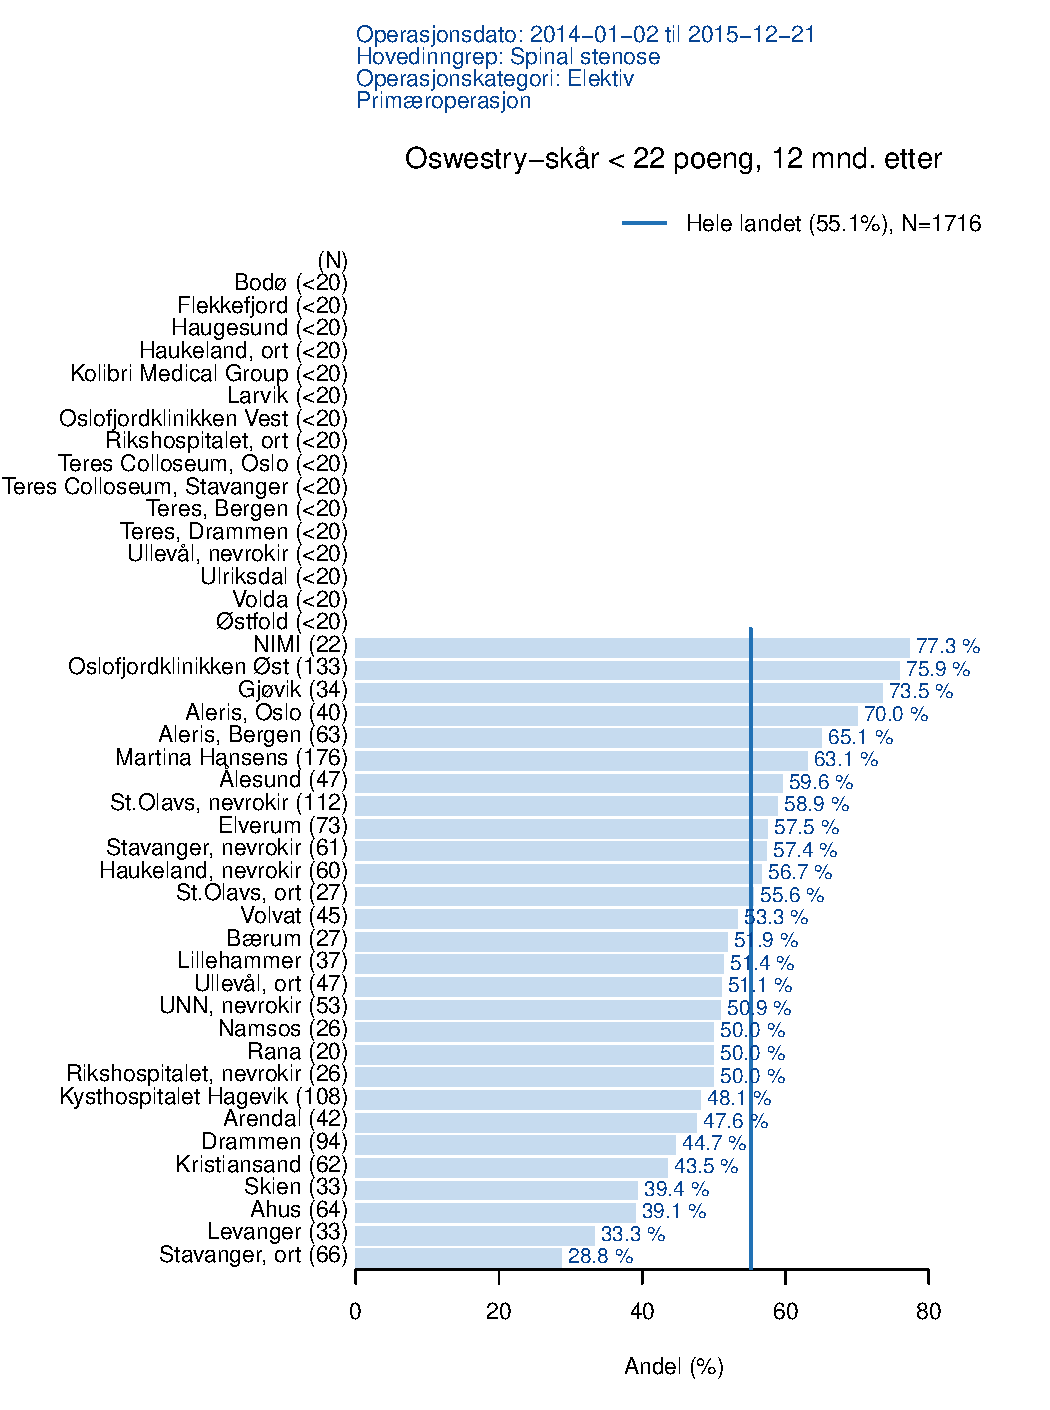
\includegraphics{Figurer/FigOsw22SS.pdf}}
\caption{\label{fig:Osw22SS}   Andel pasienter med ODI under 22 ett år
etter spinal stenose operasjon. Pasienter operert i 2015 og 2016.}
\end{figure}



\subsection{Opplevd nytte av operasjon}

% Figur \ref{fig:Nytte} viser hvor stor nytte pasientene opplever å ha hatt av behandlingen ett år etter operasjon fordelt på år. Tallet øverst på søyla angir antall pasienter som har svart. 
% I figuren er det gjort følgende aggregering av svaralternativene i spørreskjemaet:
% \begin{itemize}
% \item ''Frisk mye/bedre'' omfatter ''helt bra'' og ''mye bedre'' 
% \item ''Omtrent uendret'' omfatter ''litt bedre'', ''ingen endring'' og ''litt verre'' 
% \item ''Klart verre'' omfatter ''mye verre'' og ''verre enn noen gang før''
% \end{itemize}
Andelen som opplever at de har blitt helt bra eller mye bedre ett år etter operasjon var  henholdsvis XX\% for prolapsopererte og YY\% for spinal stenose opererte. Disse tallene har vært stabile siden 2011. Andelen pasienter som angir at de er klart verre er henholdsvis har ligget stabilt rundt ...\% for prolaps og ...\% spinal stenose opererte.

Vi ser at en mindre andel av spinal stenose pasienter opplever å ha hatt stor nytte av operasjonen sammenlignet 
med prolapspasienter.



% \begin{figure}[h] 
% \begin{center}
% \scalebox{s2}{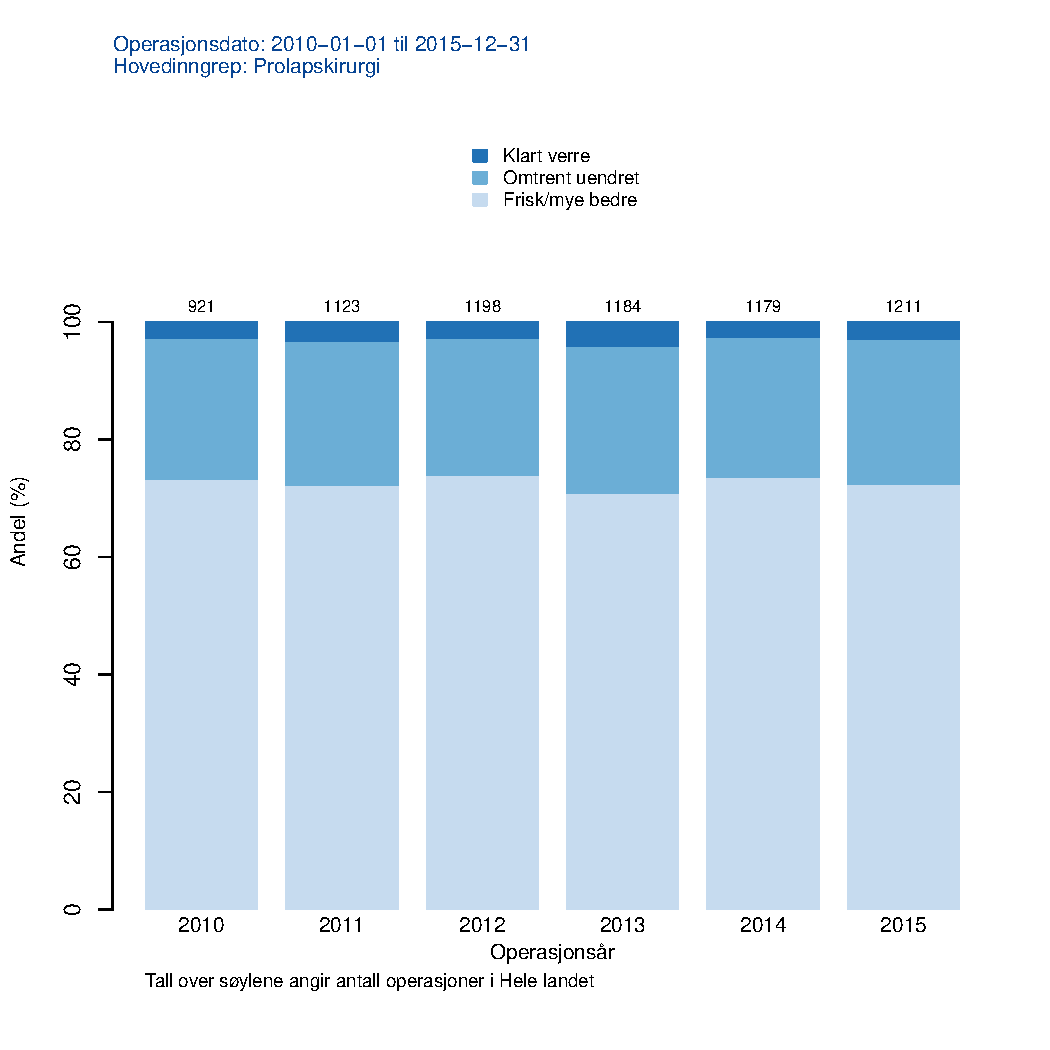
\includegraphics{Figurer/FigNyttePro.pdf}}
% \scalebox{s2}{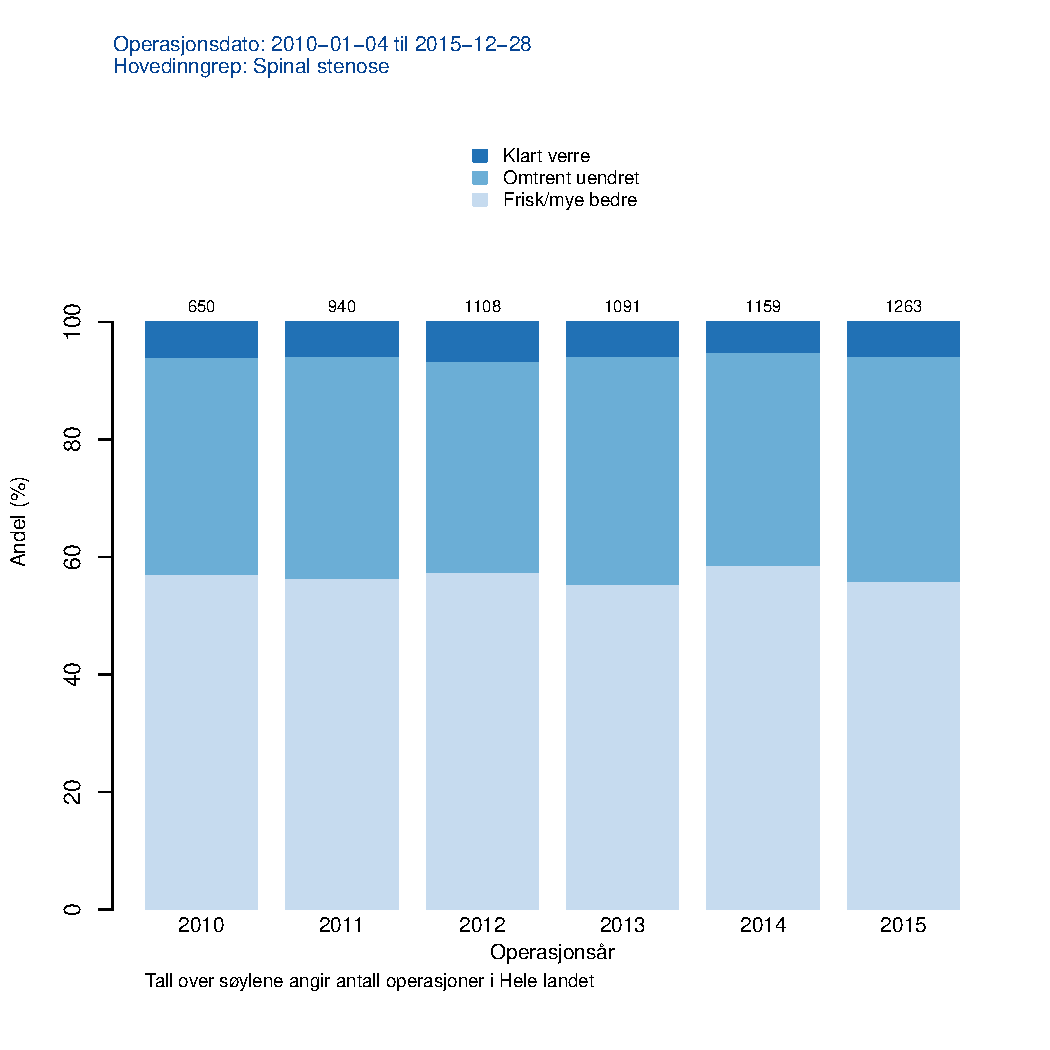
\includegraphics{Figurer/FigNytteSS.pdf}}
% \end{center}
% \caption{Spørsmål stilt 12 måneder etter operasjon til henholdsvis prolaps- og spinal stenosepasienter$:$ Hvilken nytte mener du at du har hatt av operasjonen?}
% \label{fig:Nytte}
% \end{figure}

\subsection{Pasienttilfredshet}

% Figur \ref{fig:Fornoyd} viser hvor fornøyde pasientene var med behandlinga de fikk på sykehuset ktrtxt 
% etter operasjon fordelt på operasjonsår. Tallet øverst på søyla angir antall pasienter som har svart. 
På spørreskjemaet kan pasienten angi ett av 5 svaralternativer:
\begin{itemize}
\item Fornøyd
\item Litt fornøyd
\item Hverken fornøyd eller misfornøyd
\item Litt misfornøyd
\item Misfornøyd


Andelen prolapspasienter som ett år etter behandlinga er fornøyde med behandlingen de fikk på sykehuset (PREM) 
ligger mellom 78 \% og 81 \% 
for pasienter operert i perioden 2011-2016. 
Tilsvarende ligger andel fornøyde spinal stenosepasienter mellom 73 \% 
og 77 \%
Vi ser at spinal stenose pasienter gjennomgående er litt mindre fornøyde enn prolapspasienter.






% \begin{figure}[h] 
% \begin{center}
% \scalebox{s2}{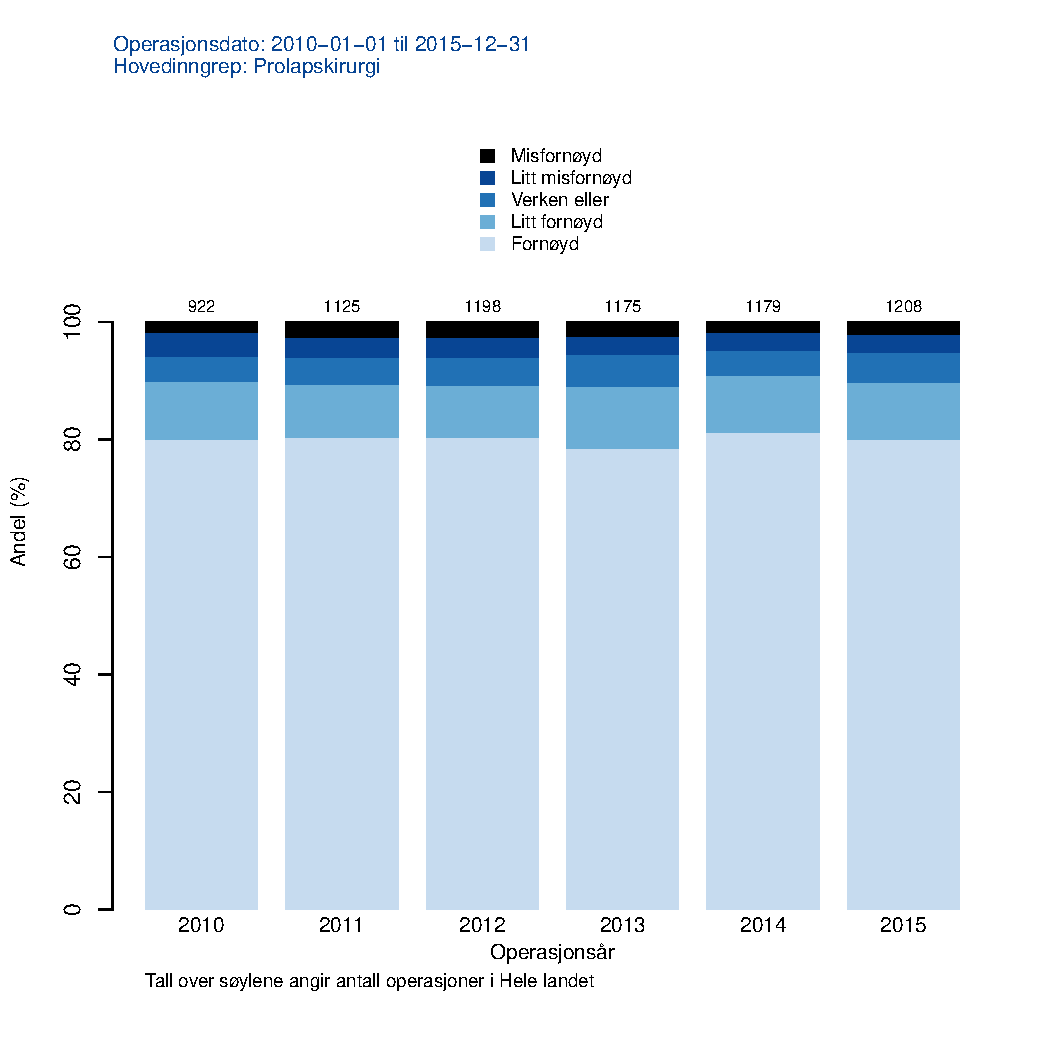
\includegraphics{Figurer/FigFornoydPro.pdf}}
% \scalebox{s2}{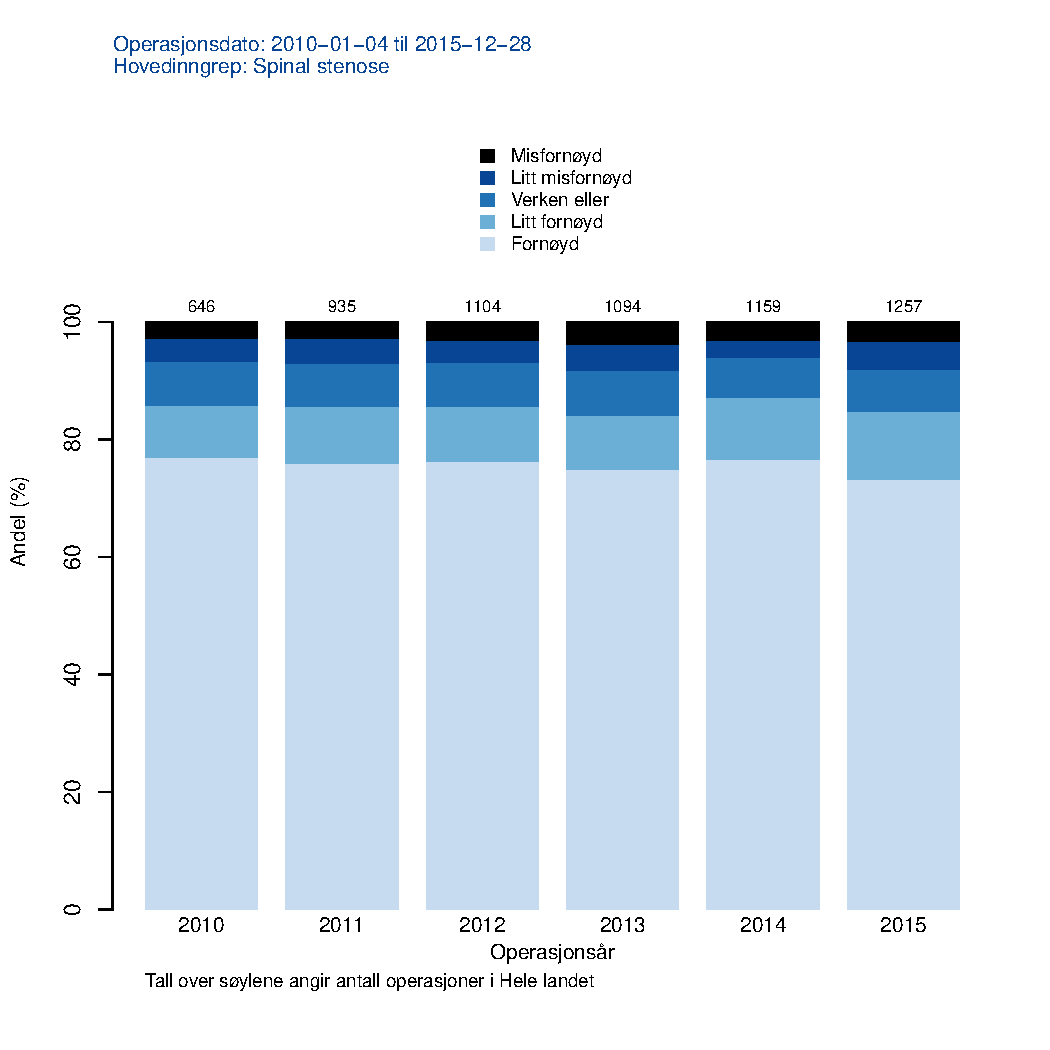
\includegraphics{Figurer/FigFornoydSS.pdf}}
% \end{center}
% \caption{Spørsmål stilt 12 måneder etter operasjon: Hvor fornøyd er du med behandlinga du har fått på sykehuset? til henholdsvis prolaps- og spinal stenosepasienter}
% \label{fig:Fornoyd}
% \end{figure}

\begin{figure}[h] 
\scalebox{0.7}{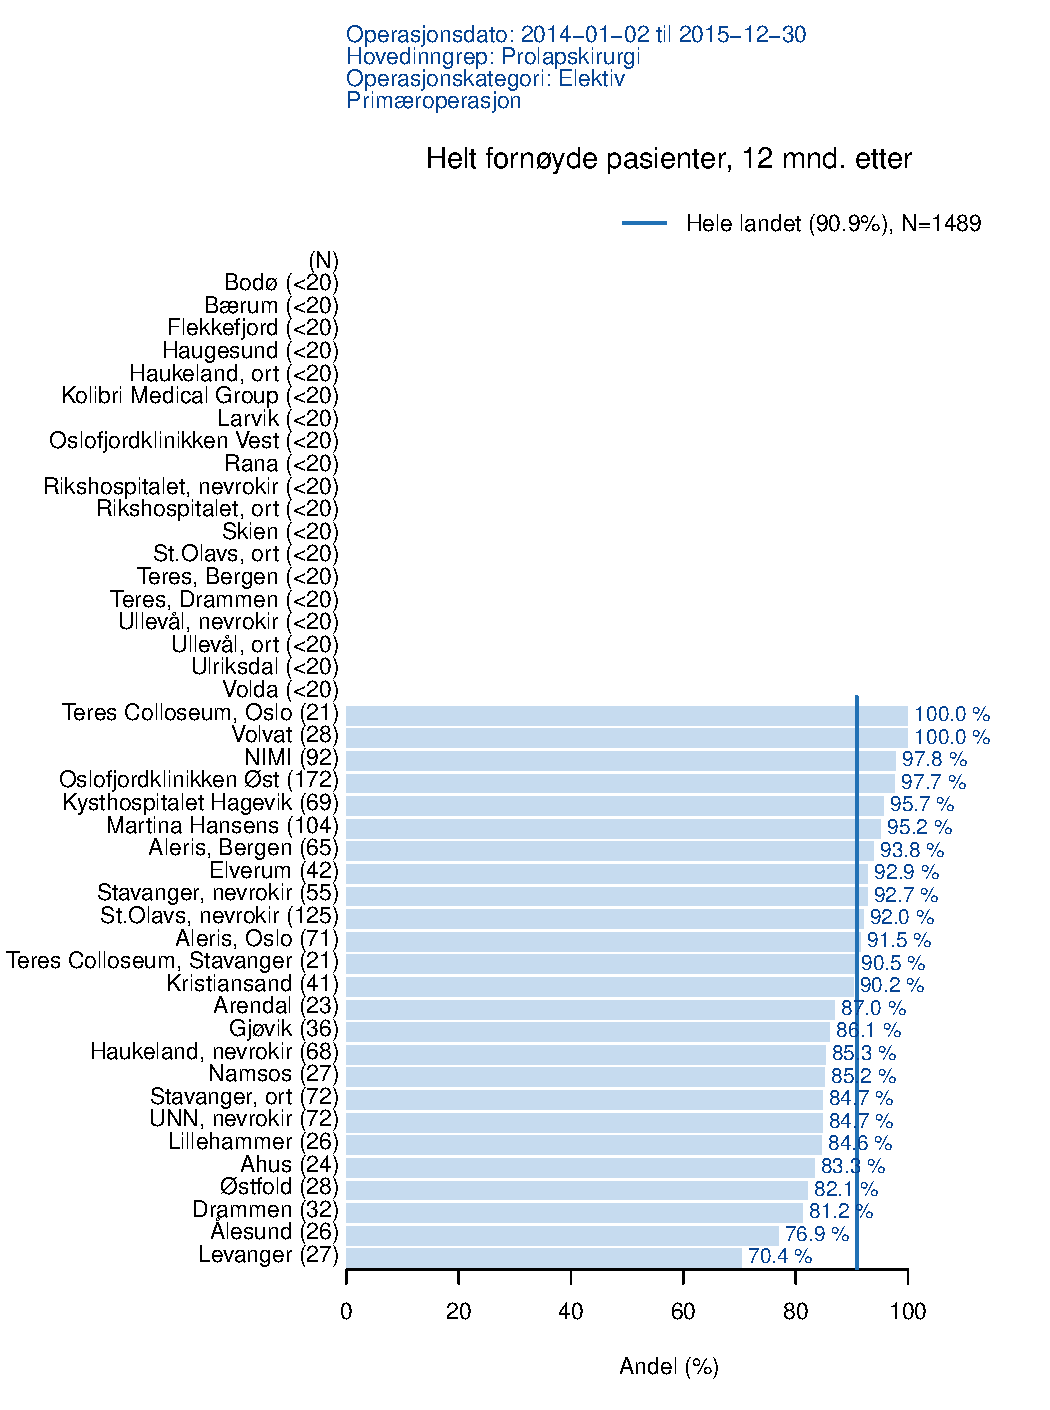
\includegraphics{Figurer/FigFornoydAvdPro.pdf}}
\caption{Prolapspasienter operert i 2014 og 2015, som ett år etter er helt fornøyde med behandlinga de har fått på sykehuset}
\label{fig:FornoydAvdPro}
\end{figure}

\begin{figure}[h] 
\scalebox{0.7}{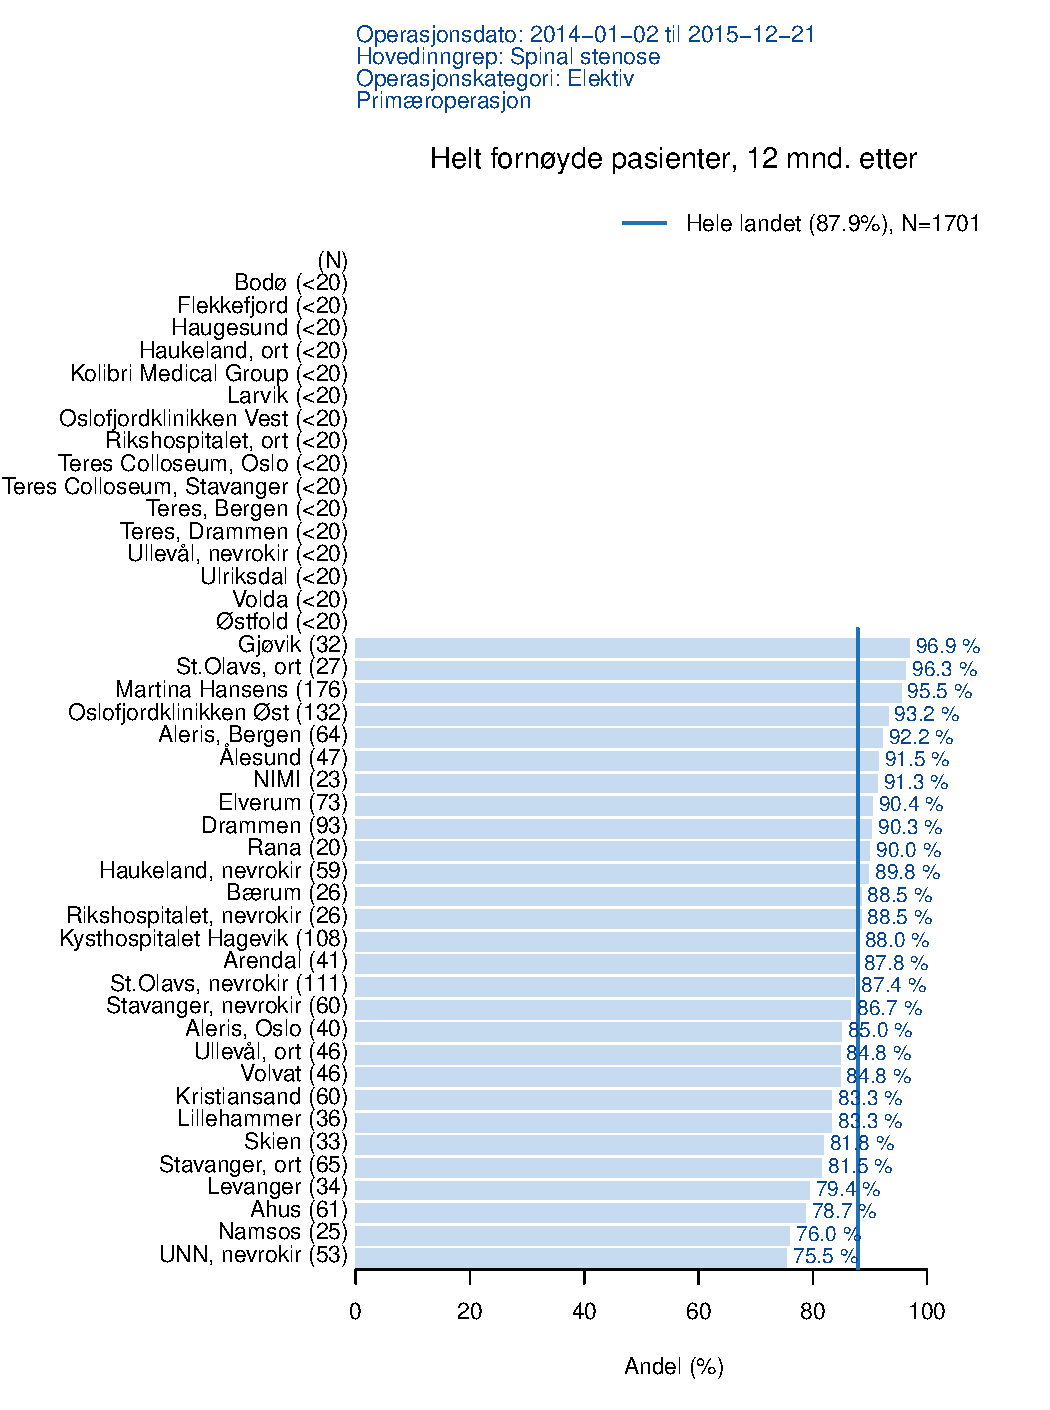
\includegraphics{Figurer/FigFornoydAvdSS.pdf}}
\caption{Spinal stenosespasienter som er helt fornøyde med behandlinga de har fått på sykehuset}
\label{fig:FornoydAvdSS}
\end{figure}


\subsection{Prolapskirurgi (alle kategorier)}



% Gjennomsnittlig liggetid på sykehus i forbindelse med prolapsoperasjon har gått ned med 
% NedgLiggetidPro døgn fra 2010 til rappAar.



\clearpage

\subsection{Kvalitetsindikatorer}
\subsubsection{Degenerativ rygg}

Det er viktig å merke seg at "indikator"  betyr en \textbf{mulig} sammenheng 
med kvalitet. Om indikatoren peker på et område som kan forbedres, må vurderes på det enkelte sykehus..

%\subsubsection{Sykehusvise resultater}



Resultatene nedenfor gjelder planlagt, første gangs operasjon for lumbal spinal stenose og prolaps.
Kun avdelinger med mer enn 10 evt. 20 (avhenger av type resultat) registrerte operasjoner i er med i
analysen.
Grunnen til at gjentatt kirurgi (reoperasjon) og øyeblikkelig hjelp (ø-hjelp)
er filtrert bort er at dette er ulikt fordelt mellom sykehusene.



Hos prolapspasienter som ikke har vært operert i ryggen tidligere er 
suksessraten 63.4 \% mot 54.8 \%
hos de som har vært operert før. 
''Suksess'' er definert som mer enn 20 poengs forbedring av ODI. 

Dersom man har vært operert mer enn 2 ganger tidligere i
ryggen, faller suksessraten for prolapsoperasjoner til 42 \% 
og for spinal stenoseopererte faller suksessraten fra 
47.6 \% til 36.3 \%. 
Sykehus som får henvist få pasienter som ø-hjelp og
mange til reoperasjon vil dermed få dårligere resultater. 
Langt færre pasienter i spinal stenosegruppen opereres som øyeblikkelig hjelp; 0.6 \%.
Hos prolapspasienter operert som ø-hjelp er andelen med betydelig forbedring 
(suksessrate)  78.7 \%, mot 57 \% av de som blir 
operert planlagt (elektivt). 




\subsubsection{God indikasjonsstilling (rett pasient)}



Pasienter som har mye plager, vil kunne forvente størst nytte av ryggoperasjon,
mens de som har lite plager vil ha mindre potensial for forbedring og større risiko
for forverring. Gevinst av kirurgi henger derfor sammen med hvor streng
indikasjonsstillingen («inngangsbilletten» til kirurgi) har vært. Figur \ref{fig:BeinsmEndrPre} viser denne
sammenhengen tydelig. Det er verdt å merke seg er at hvis pasienten har lite smerter før
operasjon (bensmerter under 3 på den horisontale smerteskalaen), er det stor
sjanse for at pasienten faktisk blir verre (mindre enn 0 på den vertikale skalaen) etter
operasjon. \\
Figur \ref{fig:BeinsmLavPre} viser at det er stor variasjon i hvor stor grad sykehusene opererer
pasienter med prolaps og lite beinsmerter. Pasienter med lammelse (parese) er tatt
ut av analysen, da de ofte må opereres uansett grad av smerte.



\begin{figure}[ht]
\scalebox{0.7}{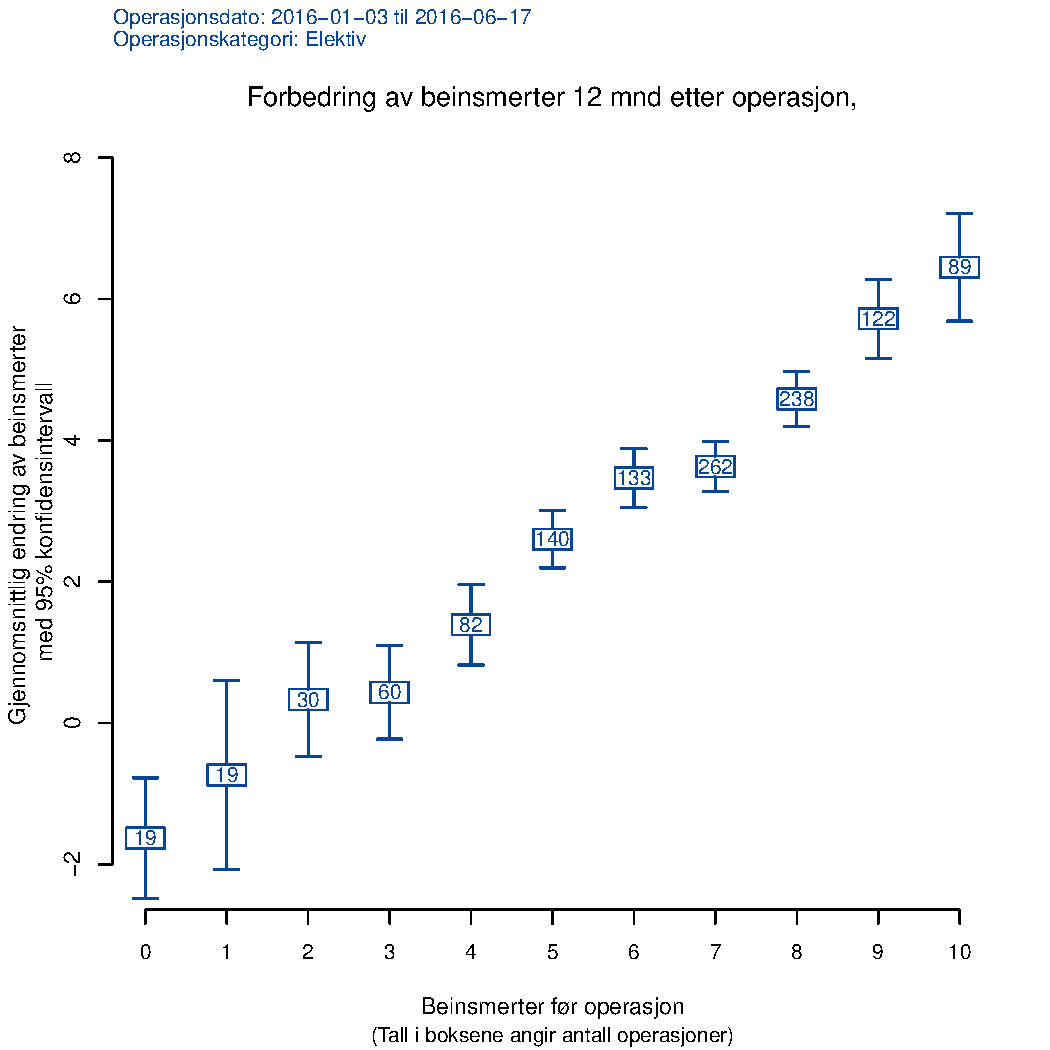
\includegraphics{Figurer/FigBeinsmEndrPre.pdf}}
\caption{\label{fig:BeinsmEndrPre}  Sammenheng mellom intensitet av bensmerte før operasjon og
forbedring etter operasjon. Skala for bensmerter går fra 0 til 10, hvor 0 betegner
ingen og 10 verst tenkelige smerte før operasjon (horisontal akse). Negativ endring
av bensmerten (vertikal akse) tilsvarer forverring, 0 betyr uendret smerte etter
operasjon.}
\end{figure}

\begin{figure}[ht]
\scalebox{0.7}{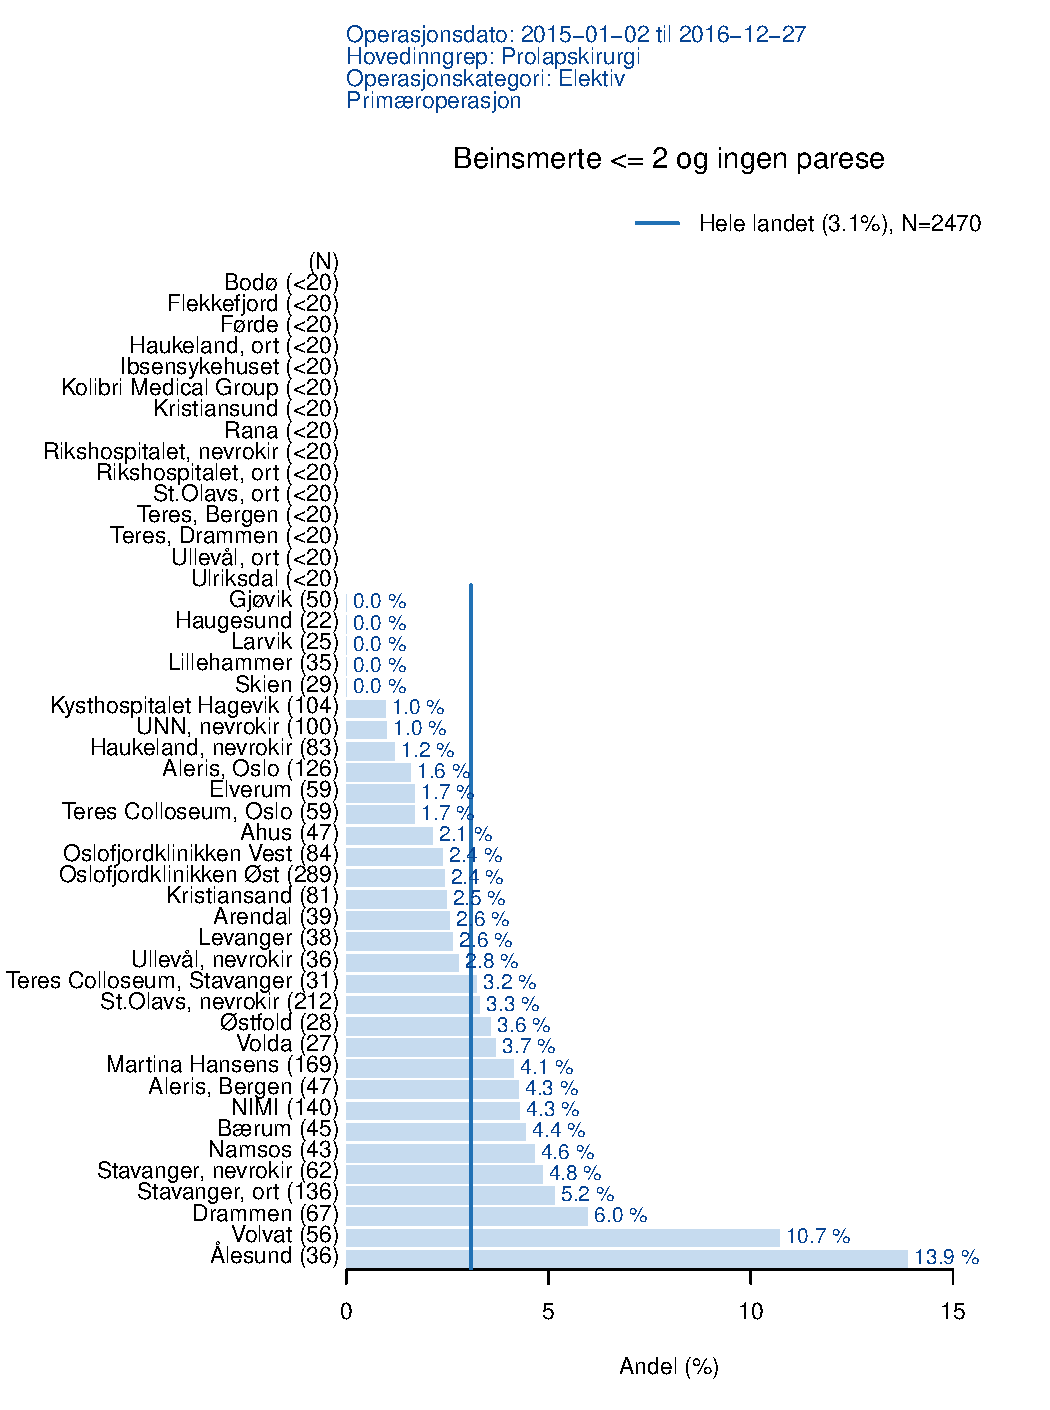
\includegraphics{Figurer/FigBeinsmLavPre.pdf}}
\caption{\label{fig:BeinsmLavPre}  Andel pasienter med lite beinsmerter ($\leq 2$) operert for prolaps.}
\end{figure}



\subsubsection{Varighet av smerter i rygg-/hofte og av utstrålende smerter på operasjonstidspunktet}

\it{Deles i Prolaps og SS?}
% latex table generated in R 3.5.0 by xtable 1.8-2 package
% Wed Sep 12 15:11:54 2018
\begin{table}[ht]
\centering
\begin{tabular}{lr}
  \hline
 & Andeler \\ 
  \hline
Ingen utstrålende smerter & 3\% \\ 
  $<$ 3 mnd & 12.4\% \\ 
  3 - 12 mnd & 35.1\% \\ 
  1 - 2 år & 18.7\% \\ 
  $>$ 2 år & 25.8\% \\ 
  Ikke besvart & 5.1\% \\ 
   \hline
\end{tabular}
\caption{Varighet av nåværende utstrålende smerter} 
\label{tab:Utstr}
\end{table}


Andelen pasienter som har hatt beinsmerter mer enn ett år på
operasjonstidspunkt av de som er registrert i NKR var uendret fra 2011 til 2017 (47\%). 
I nasjonale retningslinjer (2007) er det anbefalt å operere pasienter for prolaps før
beinsmertene har vart for lenge, helst innen ett år. Derfor bør
pasientgruppen håndteres raskt og effektivt når beslutning om operasjon er tatt og
ikke-kirurgisk behandling har vært forsøkt. Data fra NKR og nyere forskning viser at
pasienter som opereres for prolaps og har hatt beinsmerter mer enn ett år har
dårligere prognose. 
Det er stor variasjon i varighet av beinsmerter hos pasienter som blir
operert ved ulike sykehus. Det har sannsynligvis sammenheng med ventetid for
utredning og operasjon og tilgjengelig operasjonskapasitet i forhold til etterspørsel.




Tabellen  \ref{tab:Utstr} viser fordeling av hvor lenge pasientene har hatt utstrålende smerter. 
Figurene \ref{fig:VarighSmerteUtstrAvdPro} og \ref{fig:VarighSmerteUtstrAvdSS} viser hvor stor andel av henholdsvis prolaps- og spinal stenosepasienter som har hatt ustrålende smerter i mer enn ett år ved hvert sykehus. 
%Figurene \ref{fig:VarighSmerteRyggAvdPro} og \ref{fig:VarighSmerteRyggAvdSS} viser hvor stor %andel av henholdsvis prolaps- og spinal stenosepasienter som har hatt rygg-/hoftesmerter mer enn %ett år ved hvert sykehus.

\begin{figure}[h] 
\scalebox{0.7}{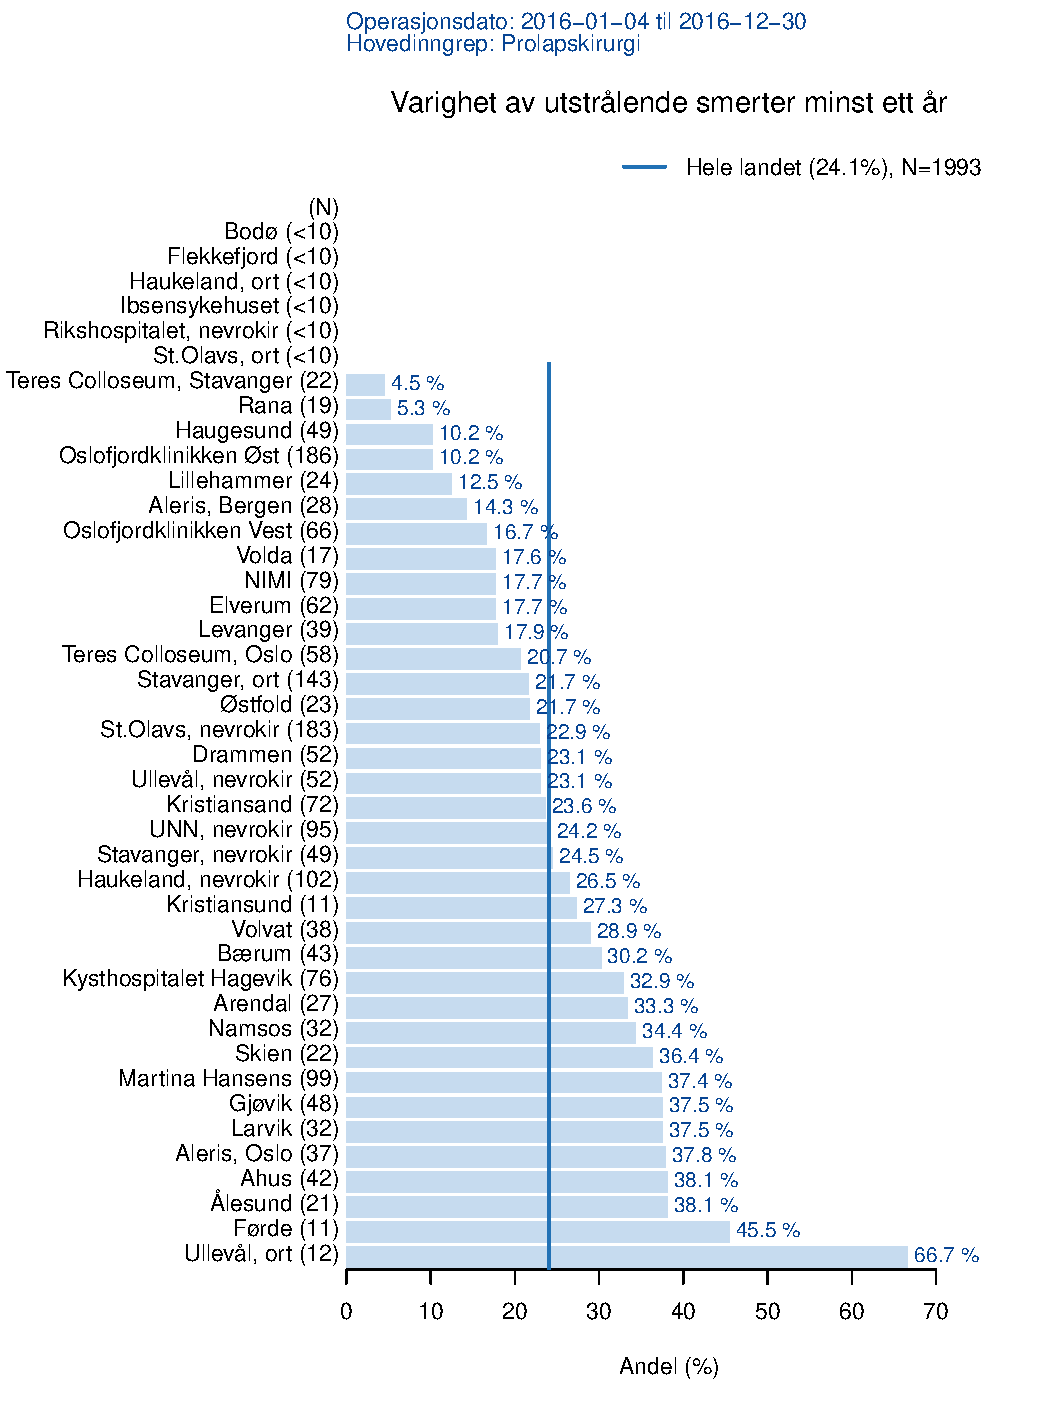
\includegraphics{Figurer/VarighUtstrAvdPro.pdf}}
\caption{Lumbale prolapspasienter som har hatt utstrålende smerter i mer enn ett år før operasjonen.}
\label{fig:VarighSmerteUtstrAvdPro}
\end{figure}

\begin{figure}[h] 
\scalebox{0.7}{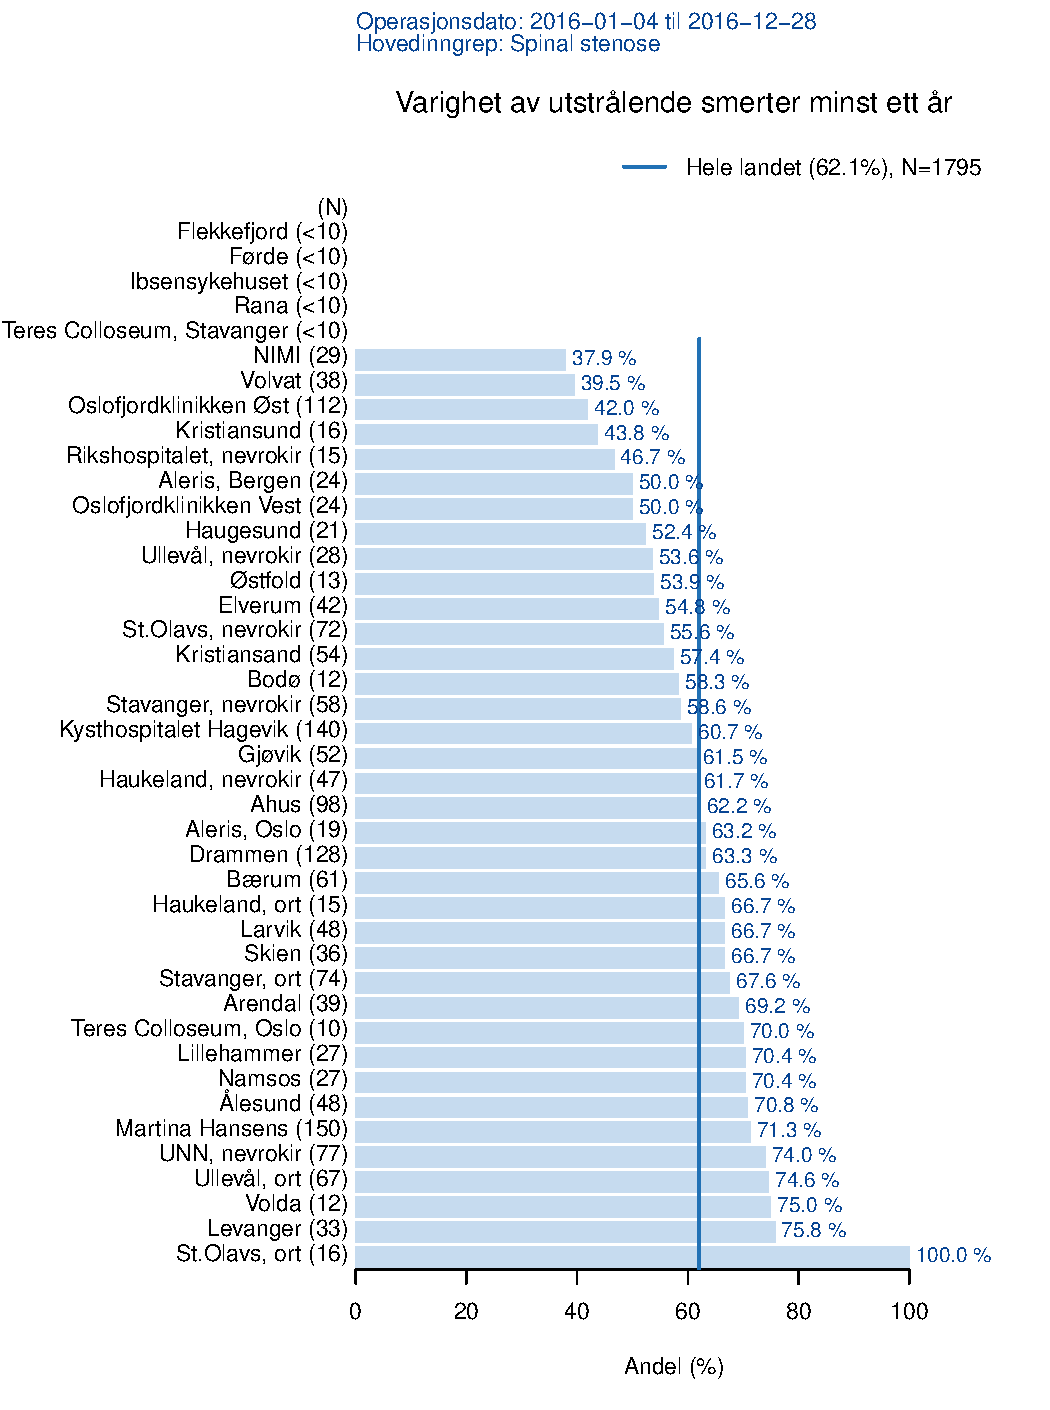
\includegraphics{Figurer/VarighUtstrAvdSS.pdf}}
\caption{Lumbal spinal stenosepasienter som har hatt utstrålende smerter i mer enn ett år før operasjonen.}
\label{fig:VarighSmerteUtstrAvdSS}
\end{figure}

Figur \ref{fig:VarighSmerteUtstrTid} viser utvikling over tid for andel pasienter med lang symptomvarighet. 

\begin{figure}[h] 
\center{
\scalebox{0.55}{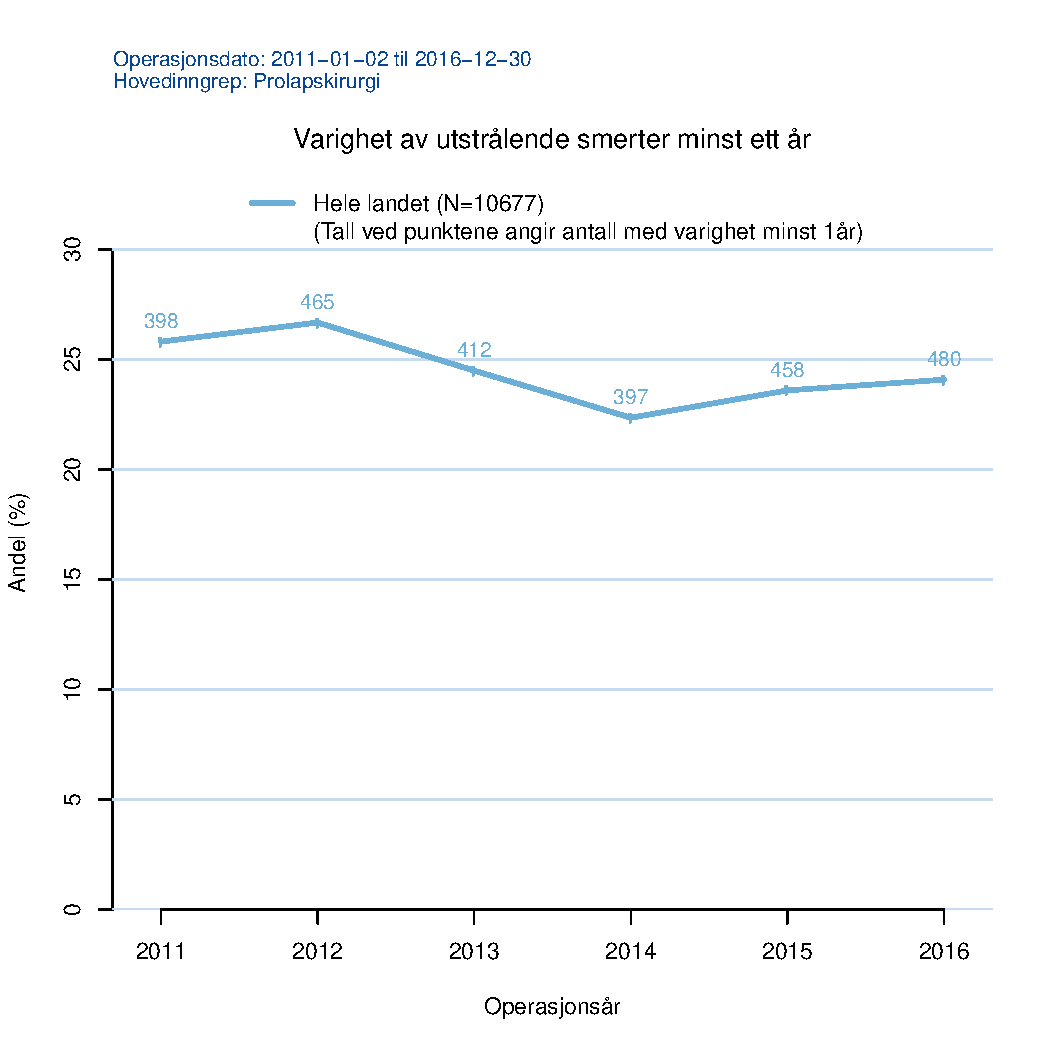
\includegraphics{Figurer/VarighUtstrTidPro.pdf}}
\scalebox{0.55}{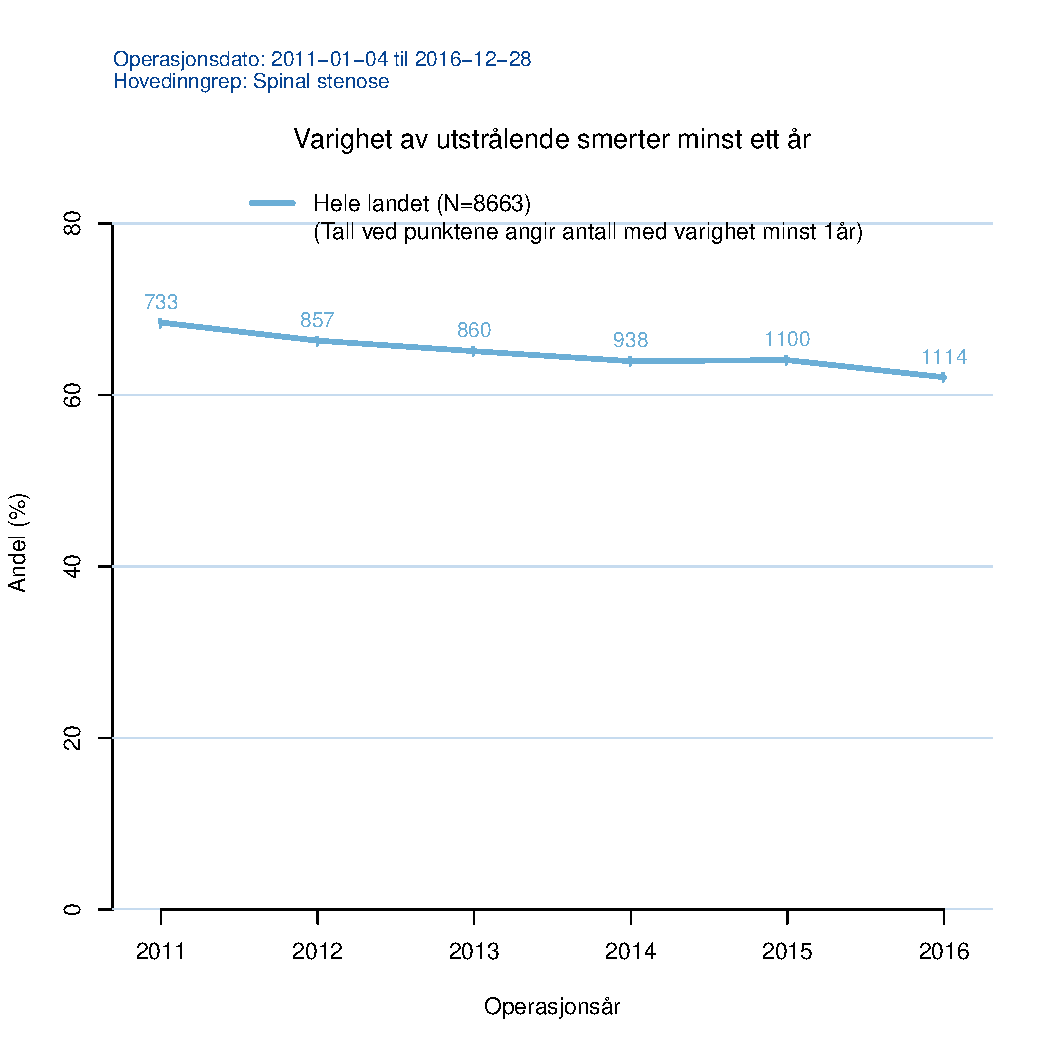
\includegraphics{Figurer/VarighUtstrTidSS.pdf}}} 
\caption{Prolaps- og Spinal stenosepasienter som har utstrålende smerter i mer enn ett år før operasjonen, utvikling over tid.}
\label{fig:VarighSmerteUtstrTid}
\end{figure}



%\begin{figure}[h] 
%\scalebox{s1}{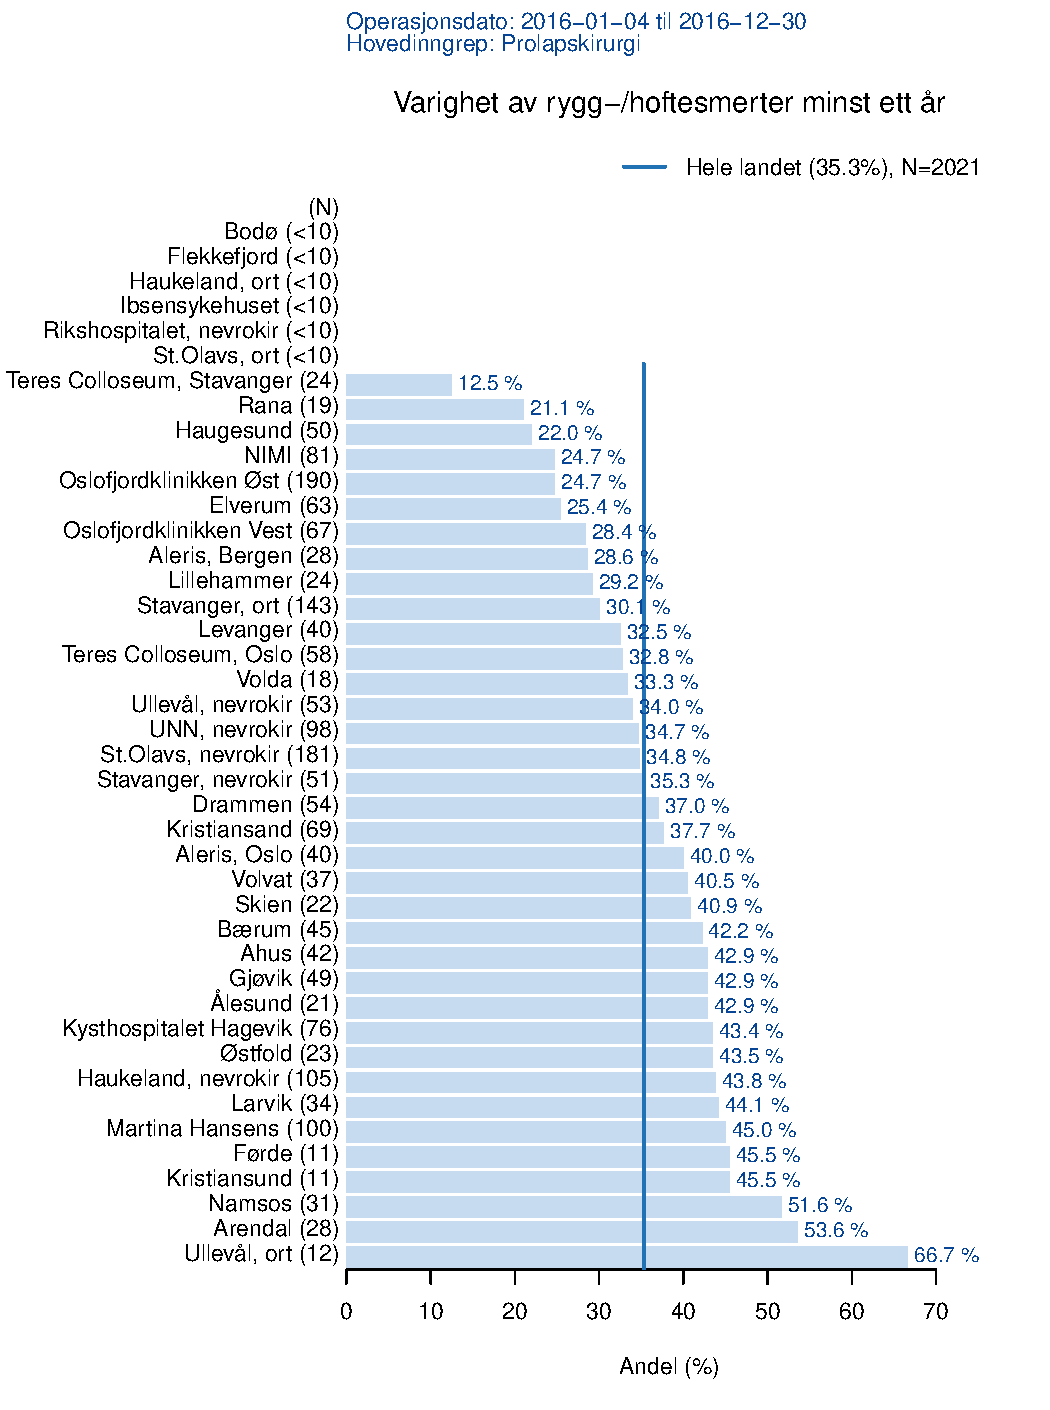
\includegraphics{Figurer/VarighRyggHofAvdPro.pdf}}
%\caption{Prolapspasienter som har hatt smerter i rygg-/hofte
%i mer enn ett år før operasjonen.}
%\label{fig:VarighSmerteRyggAvdPro}
%\end{figure}

%\begin{figure}[h] 
%\scalebox{s1}{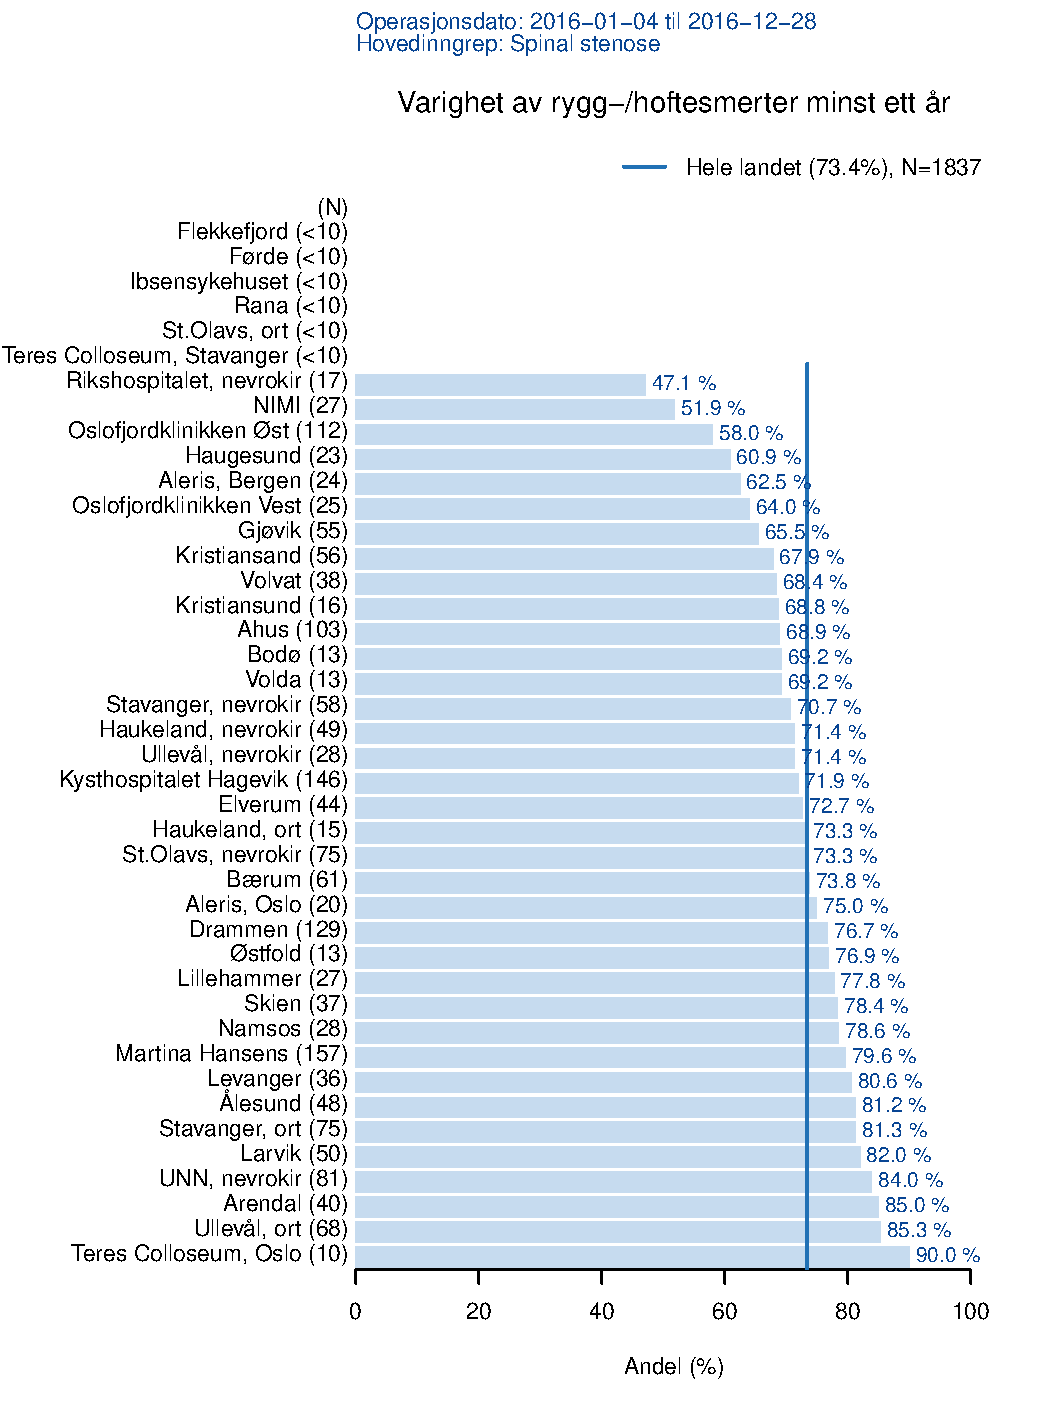
\includegraphics{Figurer/VarighRyggHofAvdSS.pdf}}
%\caption{Spinal stenosepasienter som har hatt smerter i rygg-/hofte
%i mer enn ett år før operasjonen.}
%\label{fig:VarighSmerteRyggAvdSS}
%\end{figure}




\clearpage





\subsubsection{Resultatindikatorer (behandlings-effektivitet)}

Viktige tiltak for å bedre behandlingseffektivitet vil være å øke andelen som får en
betydelig forbedring (suksessraten), redusere andelen som ikke har nytte av
behandlingen, blir verre eller får komplikasjoner. Nedenfor vises noen indikatorer
(«bench-mark kriterier») som NKR har utviklet og validert for
behandlingseffektivitet sammen med forekomst av de hyppigste komplikasjonene.
Forskjellene skyldes dels at pasientgruppene som opereres ved ulike sykehus har
ulik risikoprofil. Resultatene som vist i figurene nedenfor er ikke justert for disse
forskjellene. Kunnskap om risiko kan dette bidra til bedre utvelgelse av pasienter til
kirurgi.

\begin{knitrout}
\definecolor{shadecolor}{rgb}{0.969, 0.969, 0.969}\color{fgcolor}\begin{kframe}


{\ttfamily\noindent\bfseries\color{errorcolor}{\#\# Error: <text>:17:58: unexpected '='\\\#\# 16: \\\#\# 17: OswEndr20 <- RyggFigAndelerGrVar(RegData=RegData, aar=aar=\\\#\#\ \ \ \ \ \ \ \ \ \ \ \ \ \ \ \ \ \ \ \ \ \ \ \ \ \ \ \ \ \ \ \ \ \ \ \ \ \ \ \ \ \ \ \ \ \ \ \ \ \ \ \ \ \ \ \ \ \ \ \ \ \ \textasciicircum{}}}\end{kframe}
\end{knitrout}



% \subsubsection{Uønsket resultat}
% 
% Pasienter som 1 år etter prolapskirurgi har en ODIskår over 48 har fortsatt alvorlig
% smerterelatert funksjonshemming i dagliglivet. 
% Figur \ref{fig:Osw48} viser andelen som har ODIskår over 48 etter prolapsoperasjon. 
% Flesteparten av disse pasientene vil
% oppfatte sin livssituasjon som klart verre enn før operasjonen. 
% 
% \begin{figure}[ht]
% \scalebox{s1}{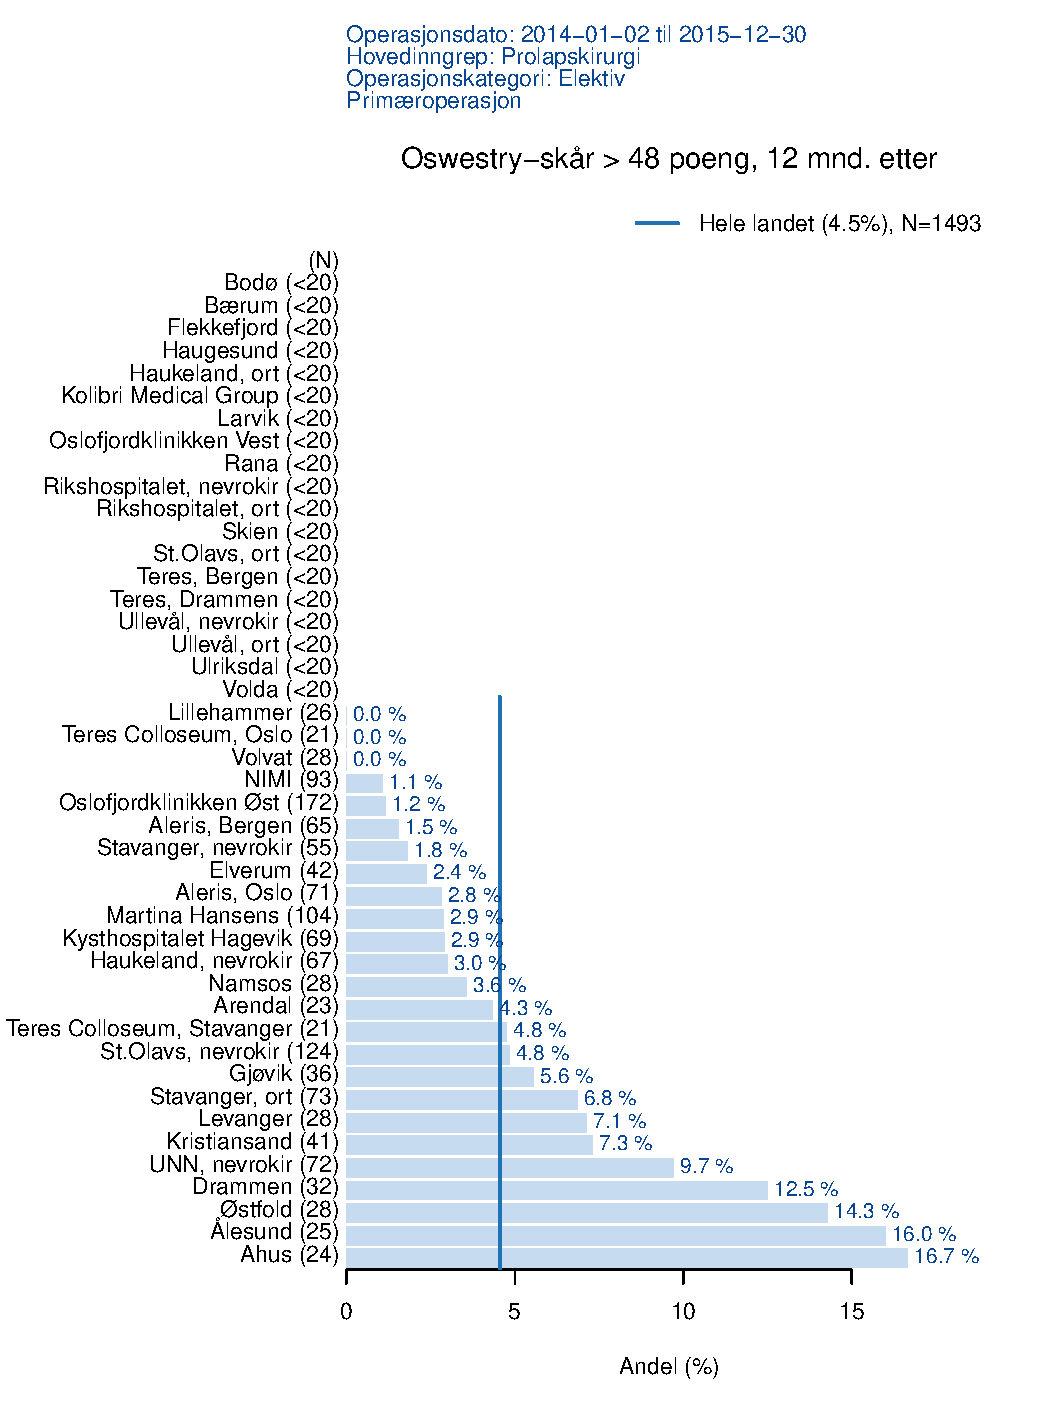
\includegraphics{Figurer/FigOsw48.pdf}}
% \caption{\label{fig:Osw48}  Andel pasienter med alvorlig smerterelatert funksjonssvikt 1 år etter
% prolapskirurgi. Pasienter operert i 2014 og 2015.}
% \end{figure}



% Pasienter med forbedring av ODI skår mindre enn 13 vil som hovedregel ikke
% oppfatte sin situasjon som vesentlig forbedret etter kirurgi. Resultatet blir dermed å
% betrakte som utilfredsstillende. Figur \ref{fig:OswEndrLav} viser andelen med lav forbedring av 
% ODI skår ved hver avdeling.
% 
% \begin{figure}[ht]
% \scalebox{s1}{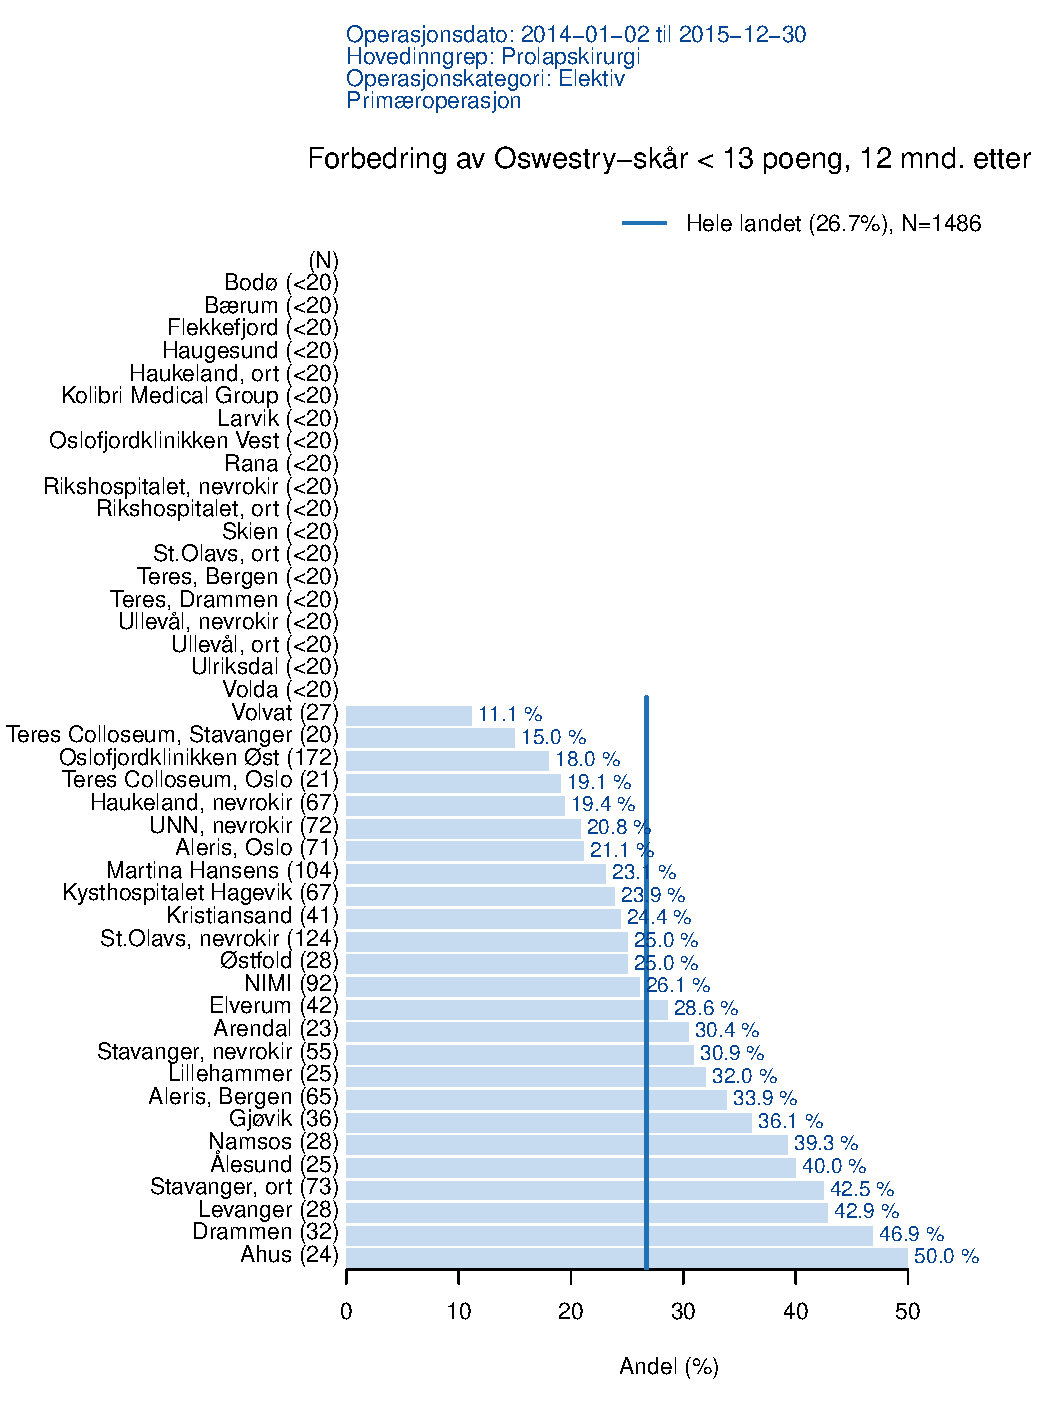
\includegraphics{Figurer/FigOswEndrLav.pdf}}
% \caption{\label{fig:OswEndrLav}   Andel pasienter som ikke oppnår et tilfredsstillende resultat, ODI
% forbedring under 13 poeng, etter prolapskirurgi. Pasienter operert i 2014 og 2015.}
% \end{figure}
% 


\subsubsection{Ønsket resultat («suksess»)}


% Figur \ref{fig:OswEndr20} viser andel pasienter med betydelig forbedring av selvrapportert
% smerterelatert funksjon i dagliglivet («suksess», ODI forbedring over 20 poeng) 1 år
% etter prolapsoperasjon.

% \begin{figure}[ht]
% \scalebox{s1}{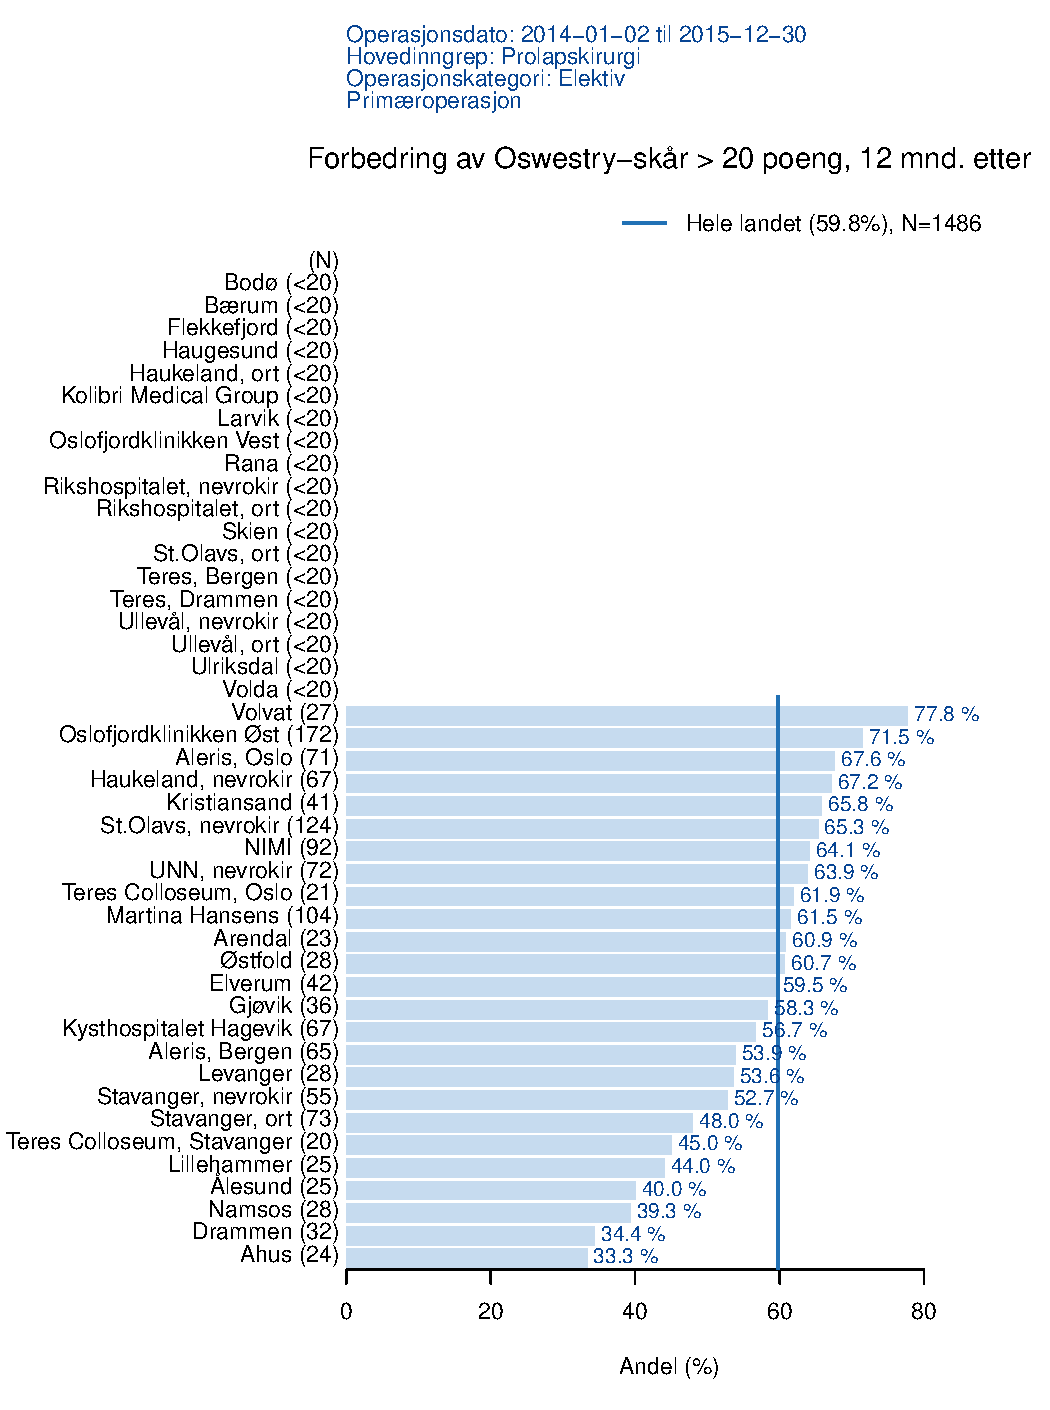
\includegraphics{Figurer/FigOswEndr20.pdf}}
% \caption{\label{fig:OswEndr20}   Andel pasienter med betydelig forbedring av selvrapportert
% smerterelatert funksjon i dagliglivet («suksess», ODI forbedring over 20 poeng) 1 år
% etter prolapsoperasjon. Pasienter operert i 2014 og 2015.}
% \end{figure}



Nyere forskning knyttet til NKR viser at pasienter operert for spinal stenose bør ha minst 30 \% forbedring av ODI for å oppleve et meget godt operasjonsresultat. Figur \ref{fig:OswEndr30pstSS} viser andelen med minst 30 \% forbedring av ODI ved hver avdeling.

\begin{figure}[ht]
\scalebox{0.7}{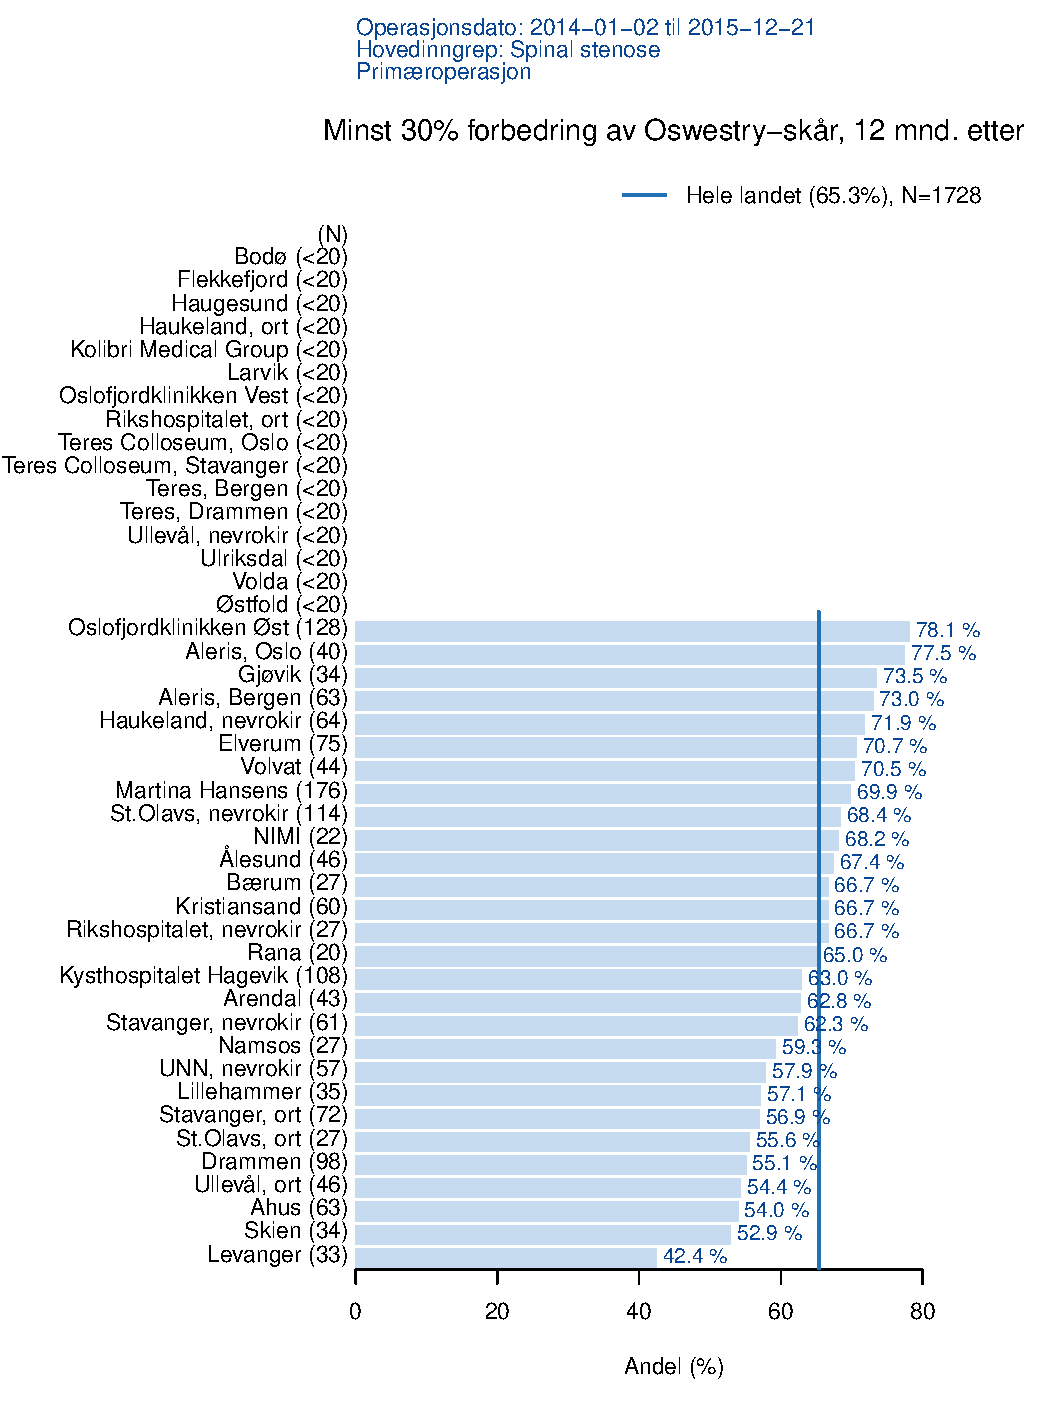
\includegraphics{Figurer/FigOswEndr30pstSS.pdf}}
\caption{\label{fig:OswEndr30pstSS} Andel spinal stenose pasienter med betydelig forbedring av selvrapportert
smerterelatert funksjon i dagliglivet («suksess», ODI forbedring over 30 \% poeng) 1 år
etter prolapsoperasjon. Pasienter operert i 2015 og 2016.}
\end{figure}













\subsubsection{Komplikasjoner (sikkerhet)}

\textbf{I. Sårinfeksjon.}

For alle typer prolapsoperasjoner har
andel sårinfeksjoner (pasientrapportert) har blitt noe redusert fram til 2011, mens bruk av  forbyggende antibiotikabehandling har økte sterkt og i dag får nesten alle forebyggende antibiotikabehandling ved kirurgi. Siden 2011 har andelen sårinfeksjoner ligget stabilt rundt 2 \% for prolapsopererte og rundt 3 \% for spinal stenose opererte.


%\begin{figure}[ht]
%      \centering \scalebox{s2}{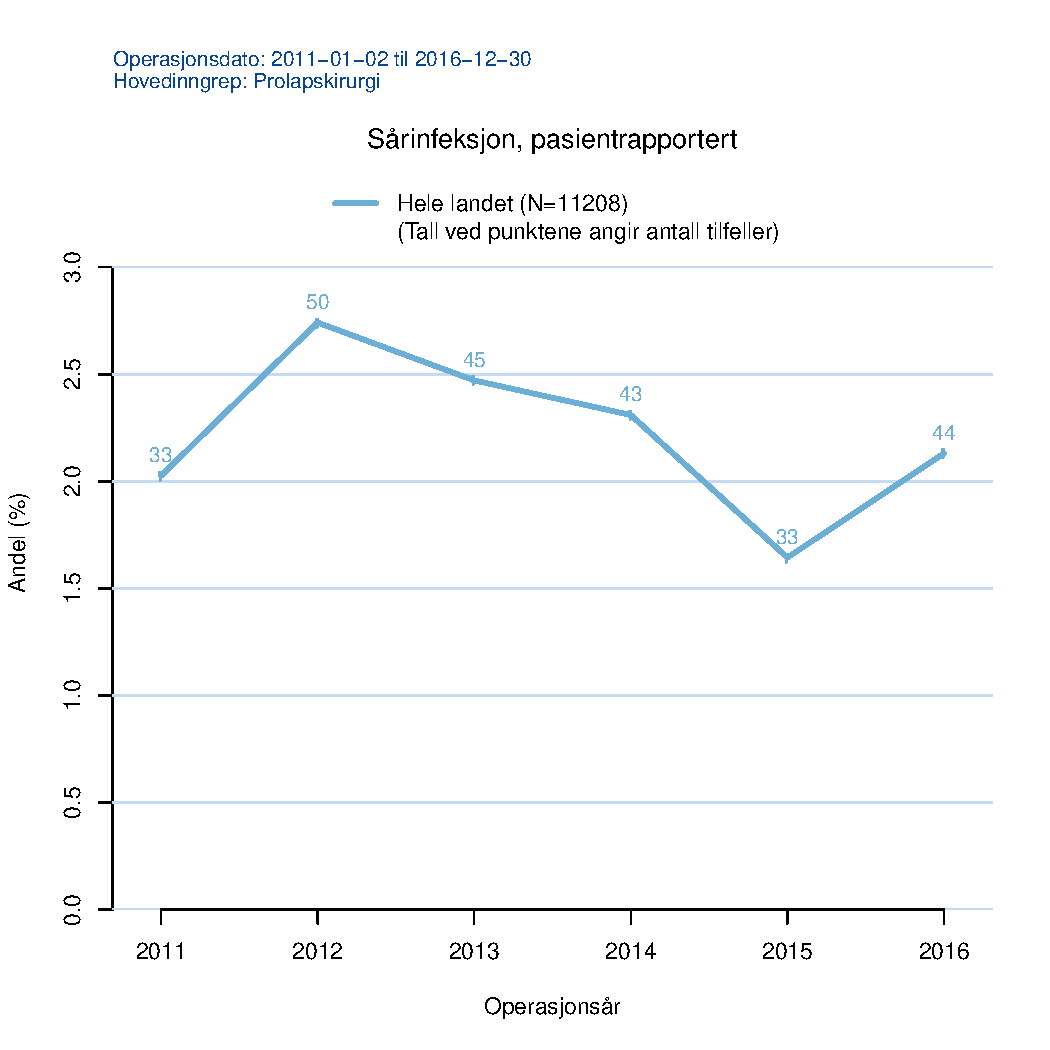
\includegraphics{Figurer/FigKpInf3MndTidPro.pdf}}
%      \centering \scalebox{s2}{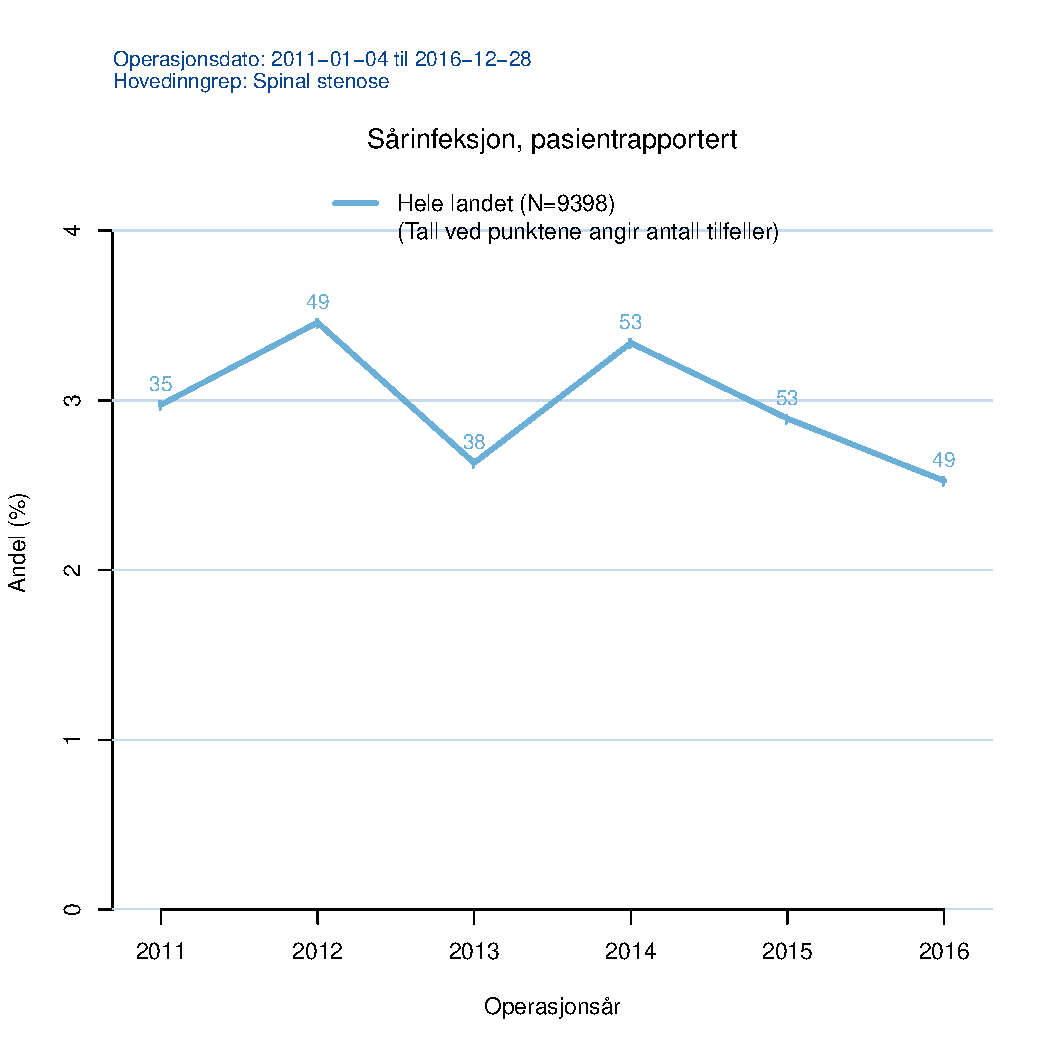
\includegraphics{Figurer/FigKpInf3MndTidSS.pdf}}
%      \caption{\label{fig:KpInfTid} Andel pasienter som rapporterer om sårinfeksjon 3 måneder etter
%hhv. prolapskirurgi og spinal stenose, utvikling over tid.}
%\end{figure}

Årsakene til sårinfeksjon er komplekse. I 2017 fikk 98-100 \% av pasienter som
opereres for prolaps, forebyggende antibiotikabehandling under operasjon. NKR
viste for mange år siden at dette har god forbyggende effekt. Figurene \ref{fig:KpInfAvdPro} og \ref{fig:KpInfAvdSS} viser andel pasienter som får sårinfeksjon ved hver avdeling.

\begin{figure}[ht]
\scalebox{0.7}{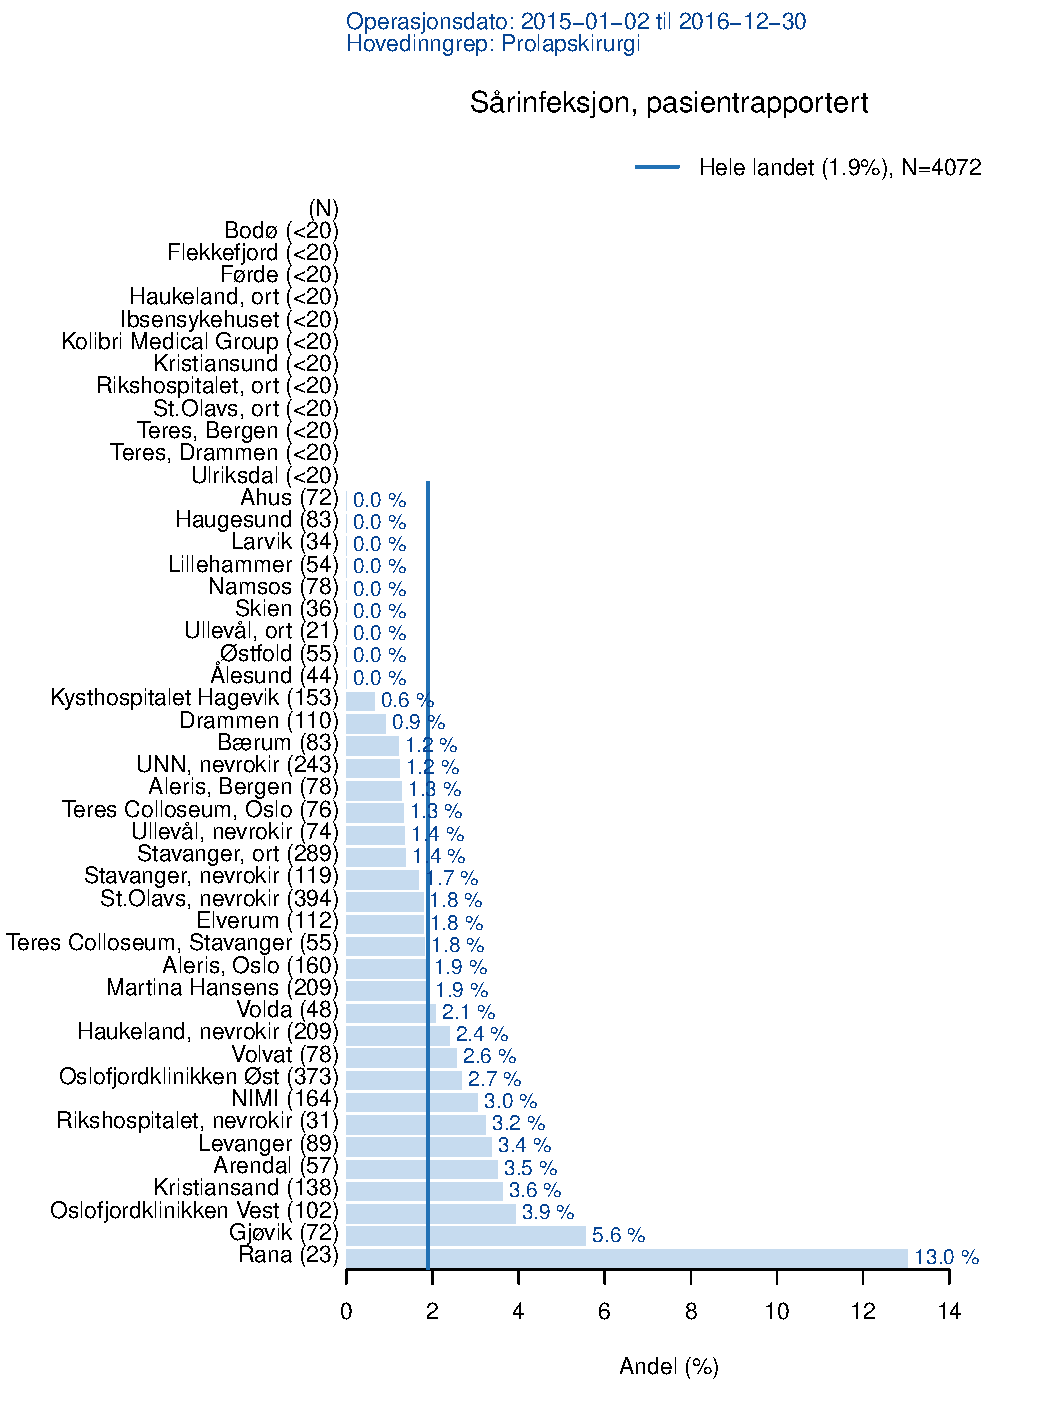
\includegraphics{Figurer/FigKpInf3MndPro.pdf}}
\caption{\label{fig:KpInfAvdPro} Andel pasienter som rapporterer om sårinfeksjon 
(overfladisk og dyp) 3 måneder etter lumbal prolapskirurgi.}
\end{figure}

\begin{figure}[ht]
\scalebox{0.7}{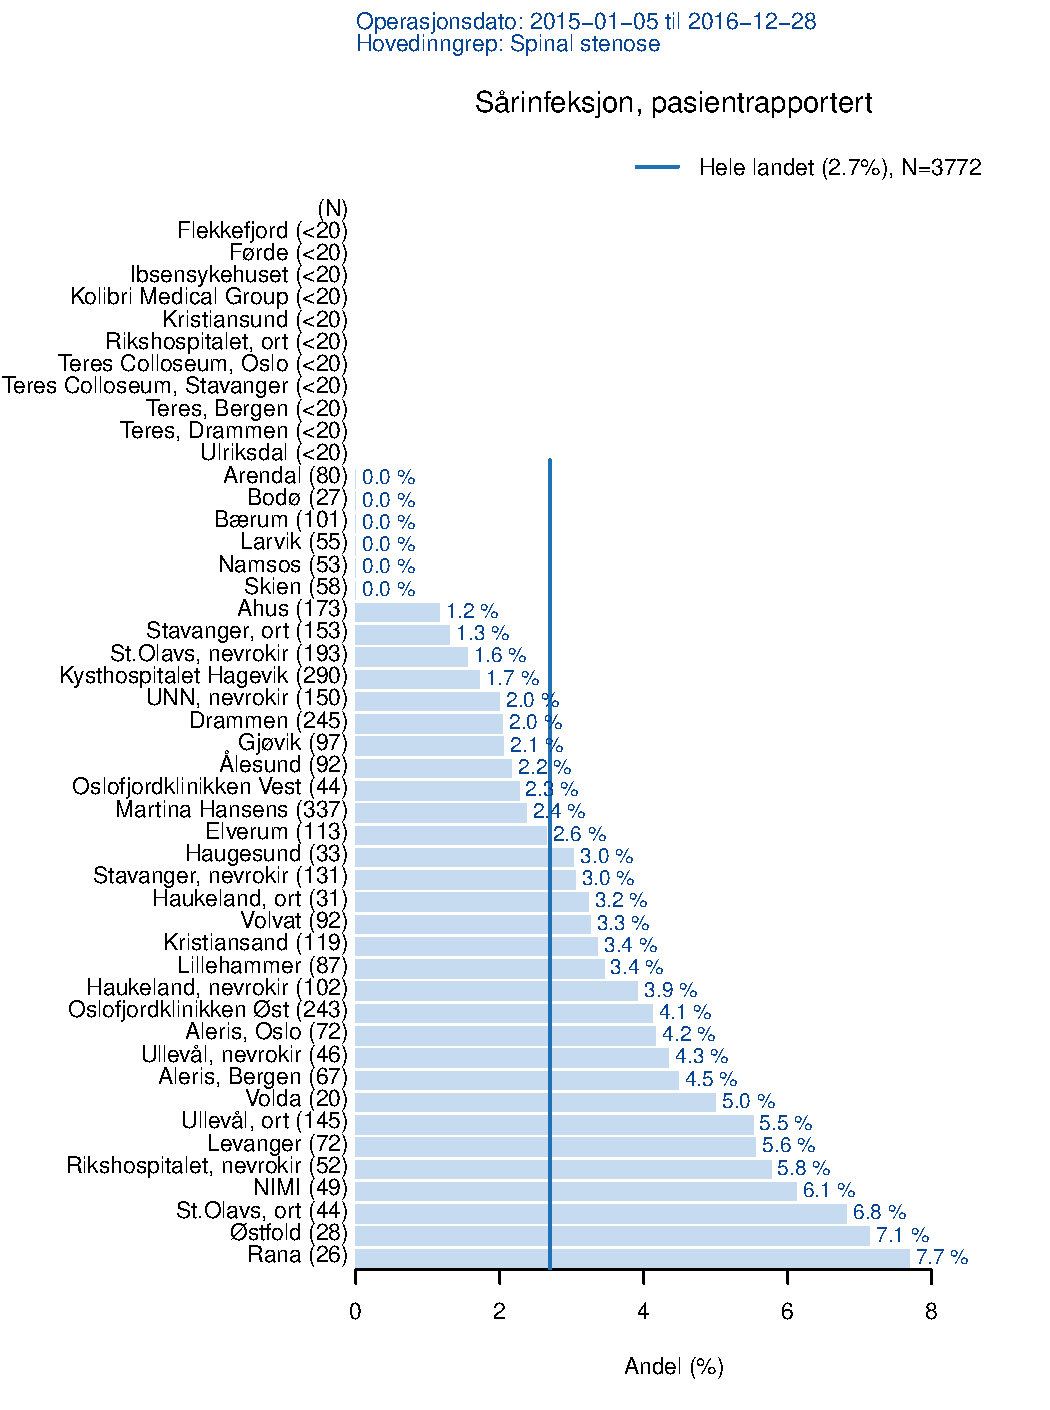
\includegraphics{Figurer/FigKpInf3MndSS.pdf}}
\caption{\label{fig:KpInfAvdSS} Andel pasienter som rapporterer om sårinfeksjon 
(overfladisk og dyp) 3 måneder etter lumbal spinal stenose operasjon.}
\end{figure}

%\clearpage



Durarift er oftest en ufarlig komplikasjon, men kan medføre væskelekkasje og
ubehag for pasienten, lengre liggetid og i noen tilfeller behov for reoperasjon.
Unntaksvis kan også konsekvensen være nerveskade og alvorlig infeksjon. Figur \ref{fig:Dura} viser andelen som får durarift for prolaps og spinal stenose pasienter.

\begin{figure}[ht]
\centering 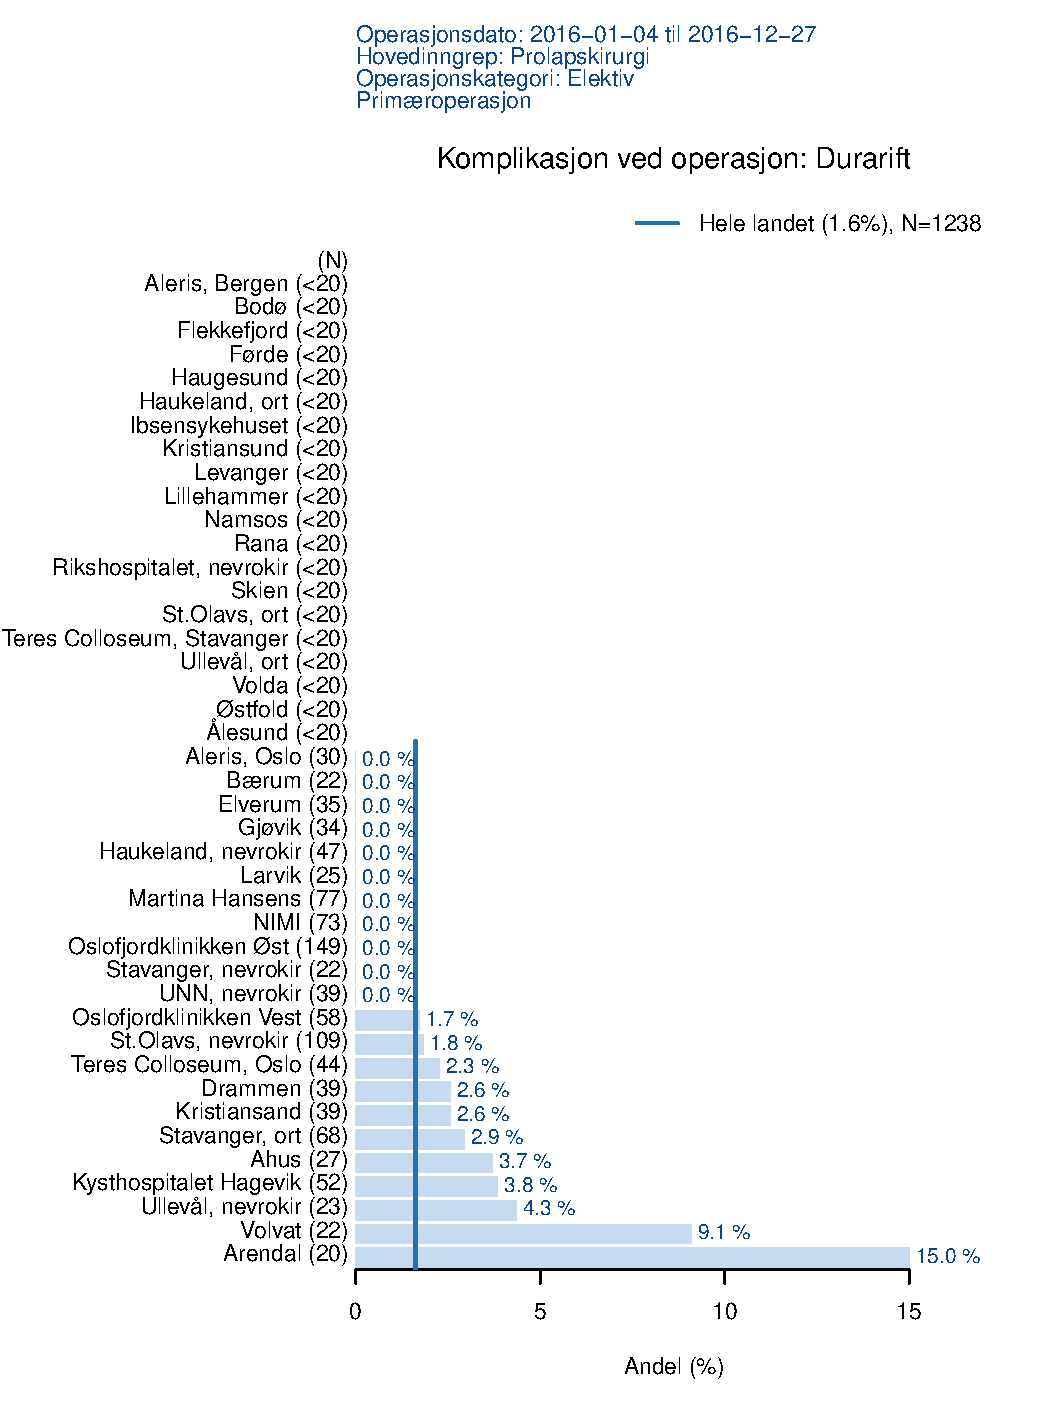
\includegraphics[width= 0.55\textwidth]{Figurer/FigDuraPro.pdf}
\caption{\label{fig:Dura} Andel pasienter som får durarift etter kirurgi for lumbalt prolaps, , elektive pasienter, ikke tidligere ryggopererte.}
\end{figure}

\begin{figure}[ht]
\centering 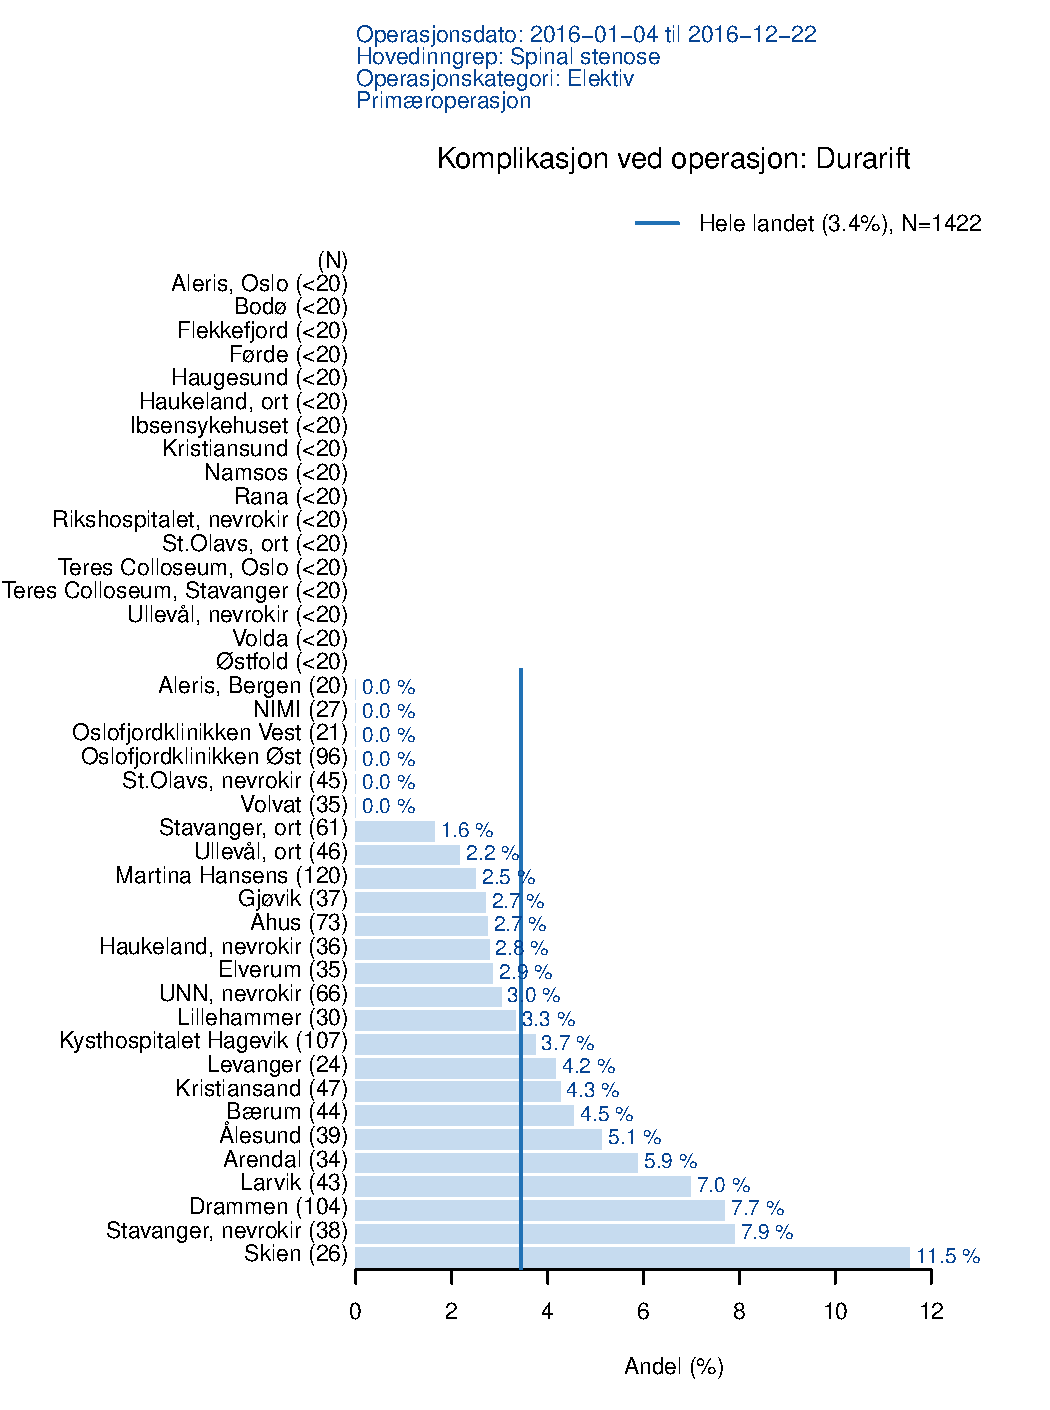
\includegraphics[width= 0.55\textwidth]{Figurer/FigDuraSS.pdf}
\caption{\label{fig:Dura} Andel pasienter som får durarift etter kirurgi for lumbal 
spinal stenose, elektive pasienter, ikke tidligere ryggopererte.}
\end{figure}








\clearpage

\section{Nakkekirurgi}
\textit{Må omskrives, Tore}

Da  det ikke finnes etablerte kvalitetsindikatorer for nakkekirurgi vil dette bli en
viktig oppgave for NKR.  Her presenteres sykehusvise data splittet på diagnose, behandling.
I Norge drives nakkekirurgi kun ved nevrokirurgiske avdelinger knyttet til de fem
universitetssykehusene i Oslo, Bergen, Trondheim, Stavanger og Tromsø, samt ved
hovedsakelig ett privat sykehus (Oslofjordklinikken, øst og vest).
Pasienter som opereres i nakken for degenerative tilstander har armsmerte med eller 
uten funksjonssvikt (radikulopati), varierende grad av nakkesmerter og noen har ryggmargspåvirkning (myelopati). 



\subsection{Bakgrunnsdata}



\subsubsection{Alder, kjønn og komorbiditet}
Gjennomsnittsalder ved nakkeoperasjon var 52 år i 2017. 46 \% var kvinner. 84 \% ble operert elektivt, planlagt kirurgi. Rundt  9 \% hadde ASA grad over II. Andelen eldre over 70 år som nakkeopereres har ligget jevnt rundt 5 \% frem til og med 2017, men varierer noe mellom sykehus, spesielt mellom offentlige og private, Figur \ref{fig:NakkeAlder70Sh}.


\begin{figure}[ht]
\scalebox{0.8}{\includegraphics{Figurer/Nakkealder70Sh.pdf}}
\caption{\label{fig:NakkeAlder70Sh} Andel nakkeopererte med alder over 70 år per sykehus}
\end{figure}

\subsection{Virksomhetsdata}

Som hovedregel kan ikke pasienter som opereres på grunn av ryggmargspåvirkning (myelopati) påregne bedring etter kirurgi i motsetning til de som behandles for nerverotspåvirkning (radikulopati). Hensikten med å operere de som har ryggmargsskade er snarere å forhindre forverring. Figur \ref{fig:NakkeOprIndikMyelopatiSh} viser at andelen som opereres for myelopati varierer mellom sykehusene.

\begin{figure}[ht]
\scalebox{0.8}{\includegraphics{Figurer/NakkeOprIndikMyelopatiSh.pdf}}
\caption{\label{fig:NakkeOprIndikMyelopatiSh} Andel nakkeoperete med diagnosen myelopati}
\end{figure}

%\subsubsection{Antibiotika}

 
% Ved bakre nakkekirurgi er det også relativt liten variasjonen i bruk av antibiotika, 
% Figur \ref{fig:NakkeAntibiotikaBakSh}. 

% \begin{figure}[ht]
% \scalebox{0.8}{\includegraphics{Figurer/NakkeAntibiotikaBakSh.pdf}}
% \caption{\label{fig:NakkeAntibiotikaBakSh} Andel som har fått profylaktisk antibiotika ved bakre nakkekirurgi ved ulike sykehus. }
% \end{figure}

\subsubsection{Sårdren}

Bruk av sårdren etter fremre nakkekirurgi har vært omdiskutert i litteraturen. Tidligere norske studier kan tyde på at bruk av sårdren er unødvendig. Figur \ref{fig:NakkeSaardrenUmFTid} viser at bruk av sårdren ved fremre nakkekirurgi er avtagende i Norge, men variasjonen mellom sykehus er stor, Figur \ref{fig:NakkeSaardrenUmFSh}.

\begin{figure}[ht]
\scalebox{0.8}{\includegraphics{Figurer/NakkeSaardrenUmFTid.pdf}}
\caption{\label{fig:NakkeSaardrenUmFTid} Andel som har hatt sårdren etter fremre nakkekirurgi i Norge per år.}
\end{figure}

\begin{figure}[ht]
\scalebox{0.8}{\includegraphics{Figurer/NakkeSaardrenUmFSh.pdf}}
\caption{\label{fig:NakkeSaardrenUmFSh} Andel som har hatt sårdren etter fremre nakkekirurgi per sykehus.}
\end{figure}

\subsection{Resultatmål}

Pasientene er fulgt opp med spørreskjema 3 og 12 måneder etter kirurgi.
Resultatene er ikke justert for forskjeller i pasientpopulasjonene.
I litteraturen er vanligvis bruk av profylaktisk antibiotikabehandling  anbefalt ved 
nakkekirurgi. Andelen som får dette har ligget stabilt over 96 \% i Norge frem til og med
\Sexpr[rappAar}.

\subsubsection{Sårinfeksjon etter bakre nakkekirurgi}


En av de hyppigste komplikasjonene etter nakkekirurgi er sårinfeksjon. Forekomsten i 2017 var 7 \% (totalt for bakre og fremre nakkekirurgi). 
\textit{LENA sjekk}, 
Ved  3 måneders etterkontroll svarer pasientene selv 
på to spørsmål  for å kartlegge dette: ''Ble du behandlet med antibiotika for overfladisk sårinfeksjon i operasjonssåret i løpet av de 4 første ukene etter operasjonen?" og 
''Har du blitt eller blir du behandlet i over 6 uker med antibiotika for dyp infeksjon i operasjonssåret?''   Andelen som har svart ja, ved hvert sykehus, på minst ett av disse spørsmålene er vist i Figur \ref{fig:NakkeKomplinfek3mndSh}.  


%\subsubsection{Sårinfeksjon}

\subsubsection{Resultat etter fremre nakkekirurgi for nerverotssmerte og funksjonssvikt (cervical radikulopati)}

Neck Disability Index (NDI) er et godt validert mål for å vurdere bedring i smerterelatert
funksjonshemming  i dagliglivets aktiviteter samt sykdomsspesifikk livskvalitet hos 
nakkeopererte. Til å måle armsmerteintensitet før og etter operasjon brukes numerisk 
smerteskala (NRS, 0-10). Figurene nedenfor viser resultater etter fremre nakkekirurgi hos 
pasienter som har nerverotssmerte og funkssjonsvikt (radikulopati) uten tegn til 
ryggmargsskade 
(myelopati). Figur \ref{fig:NakkeNRSsmerteArmEndr12mndUmFSh} og  
\ref{fig:NakkeNDIendr12mndUmFSh} at viser at mellom 60 og 70 \% har en betydelig forbedring av 
armsmerte og funksjonssvikt (NRS og NDI reduksjon tilsvarende 30 \%  eller mer) ett år etter 
kirurgi. Det et er variasjon i resultater mellom sykehus. Over 80 \% av pasientene er fonøyde 
med behandlingen de fikk, Figur \ref{fig:NakkeFornoydBeh12mndFremSh}.  

\subsubsection{Komplikasjoner etter fremre nakkekirurgi}
De hyppigste komplikasjonene etter fremre nakkekirurgi er svelg og stemmevansker som følge 
av nervepåvirkning og arrdannelser. Ved etterkontroll etter 3 måneder svarer pasientene på
følgende spørsmål: ''Har du etter operasjonen vedvarende problemer med stemmen din 
(f.eks. hesthet/svak stemme)? " og " Har du etter operasjonen hatt vedvarende ubehag ved svelging av mat og drikke? "
Andelen som har svart ja på disse to spørsmålene er henholdsvis 9 \% og 15 \%, men dette  varierer mellom sykehus, Figur \ref{fig:NakkeStemme3mndSh} og \ref{fig:NakkeSvelg3mndSh}. Årsaken til disse forskjellene er uklar. 

textit{LENA sjekk \%}



\begin{figure}[ht]
\scalebox{0.8}{\includegraphics{Figurer/NakkeNDIendr12mndUmFSh.pdf}}
\caption{\label{fig:NakkeNDIendr12mndUmFSh} Andel pasienter som har fått betydelig bedring av fysisk funksjon i dagliglivet etter fremre nakkekirurgi.}
\end{figure}

\begin{figure}[ht]
\scalebox{0.8}{\includegraphics{Figurer/NakkeNRSsmerteArmEndr12mndUmFSh.pdf}}
\caption{\label{fig:NakkeNRSsmerteArmEndr12mndUmFSh} Andel som har fått betydelig bedring av nerverotsmerte  etter fremre nakkekirurgi.}
\end{figure}

\begin{figure}[ht]
\scalebox{0.8}{\includegraphics{Figurer/NakkeFornoydBeh12mndFremSh.pdf}}
\caption{\label{fig:NakkeFornoydBeh12mndFremSh} Andel pasienter som er godt fornøyd med behandlingen de fikk på sykehuset.}
\end{figure}

\begin{figure}[ht]
\scalebox{0.8}{\includegraphics{Figurer/NakkeStemme3mndSh.pdf}}
\caption{\label{fig:NakkeStemme3mndSh} Andel pasienter som rapporterer stemmeproblemer 3 måneder etter fremre nakkekirurgi.}
\end{figure}

\begin{figure}[ht]
\scalebox{0.8}{\includegraphics{Figurer/NakkeSvelg3mndSh.pdf}}
\caption{\label{fig:NakkeSvelg3mndSh} Andel pasienter som rapporterer svelgproblemer 3 måneder etter fremre nakkekirurgi.}
\end{figure}

\begin{figure}[ht]
\scalebox{0.8}{\includegraphics{Figurer/NakkeKomplinfek3mndSh.pdf}}
\caption{\label{fig:NakkeKomplinfek3mndSh} Andel pasienter som rapporterer om sårinfeksjon 3 måneder etter nakkekirurgi.}
\end{figure}

\clearpage








\end{document}
